\chapter{Results and Discussion}
\label{chap:results}

This chapter gives an overview of the achieved results from all considered scenarios. The two parameters,
flying height and number of users, are evaluated by monitoring the power consumption, electromagnetic exposure and \gls{SAR}-values.
This is done for the two considered antennae who can both operate in two optimization strategies, making a total of four possible configurations.
These configurations will be investigated in three different scenarios.
The first section talks about Scenario I which is a small network with only one user and one \gls{UABS}. In 
the following section, Scenario II is investigated where the network is expanded for a larger population 
but with still only one \gls{UABS} available.
The network in the last section investigates Scenario III which serves a large population with an unlimited number of \gls{UABS}s.

The electromagnetic radiation and \gls{SAR} are 
measured for the weighted average user. This means that 
equation \ref{eq:em} is used with both $w_{1}$ and $w_{2}$ set to 50\%. Doing so will not only optimize the network 
towards the average user but also limit higher electromagnetic radiation. Each simulation is repeated 20 times. 
Therefore, the values for the weighted average user will be averaged over these 20 simulations.

Some interesting values are presented to give the reader an idea on how long these computations take.
For example, the variable flying height in each scenario ranges from 
20 m to 200 m in steps of 20 m resulting in a total of 200 simulations for one scenario. 
This results in more than 15 million 52 thousand path loss calculations.
The evaluated parameter  `number of users'
ranges from 50 to 600 in steps of 50, resulting 
in 240 simulations. Such one scenario takes 48 million 750 thousand path loss calculations. Remember that path loss calculations
are done in the preparation phase and the network has not even been optimized at this point.

%%%%%%%%%%%%%%%%%%%%%%%%%%%%%%%%%%%%%%%%%%%%%%%%%%%%%%%%%%%%%%%%%%%%%%%%%%%%%%%%%%%%%%%%%%%%%%%%%%%%%%%%%%%%%%%%%%%%%%%%%%%%%%%%%%%%
\section{Scenario I: One User and One \gls{UAV}}
The network contains only one user in this scenario. This means that there is only one location possible for the \gls{UAV},
being just above 
the user. This section will investigate minimal required transmission power and SAR values from different sources.
Finally, also the power consumption of the entire network is measured. The  ``entire network" refers to all \gls{UABS}s. 
For this scenario, the entire network 
will be constructed out of a single \gls{UABS}.

\subsection{The Influence of the Maximum Transmission Power}
\label{s1a}
\gls{LTE} makes use of power control meaning that no more power will be used than strictly necessary. The actual 
transmission power $P_{tx}$ therefore ranges between zero dBm and the maximum allowed input power. $P_{tx}$ is zero dBm when the \gls{UABS} does not cover anybody.
For instance when the flying height is too high and therefore also the path loss that comes with it, the maximum allowed $P_{tx}$ is not enough to cover 
the distance. In such case, the \gls{UABS} is shut down since it cannot meet the requirements.
Increasing the maximum transmission power will not influence the actual used $P_{tx}$ because the \gls{UABS} will not use more
than strictly required. It is therefore more useful to match the actual transmission power against a variable flying height. 

Figure \ref{fig:ptxfh} shows a logarithmic relationship between $P_{tx}$ and flying height.
As already discussed in \ref{sec:scenarios_s1}, the user is outdoor and just below the \gls{UABS}. There is thus a free \gls{LOS} between both
radiators. It is clear from figure \ref{fig:ptxfh} that a discontinue step function is achieved. This is because multiple flying heights correspond to the same transmission power.
When the flying height increases, so does the path loss. This causes the \gls{SNR} to drop under the required boundary.
 \gls{LTE} tries to counteract this by increasing the power level. Each time 
the path loss becomes too high, the power level of the transmitter increases with one dBm. 
Doing so, increases the \gls{SNR} allowing the user to properly receive and decode the signal again.
After a jump in the step function, there is an overestimation meaning the $P_{tx}$ increased more than necessary. So multiple flying heights correspond with the same $P_{tx}$.
Further, dBm is also a logarithmic scale meaning that while 10 dBm equals 10 mW, 20 dBm equals 100 mW. This explains why the black lines become longer at higher flying altitudes.
Each time the power level increases with one dBm, the overestimation becomes larger. If the tool would make use of a smaller step size, a more continuous 
logarithmic function would be achieved. This would however worsen the time complexity because it would take much more iterations before 
the power level exceeds the path loss. 
The red line in figure \ref{fig:ptxfh} indicates the default maximum transmission power of 33 dBm used during simulations as 
defined in table \ref{table:defaultconf}. 
In a free \gls{LOS} scenario with only one user, a \gls{UABS} can fly up to 387 metres before losing connection.

\begin{figure}[h]
  \centering
  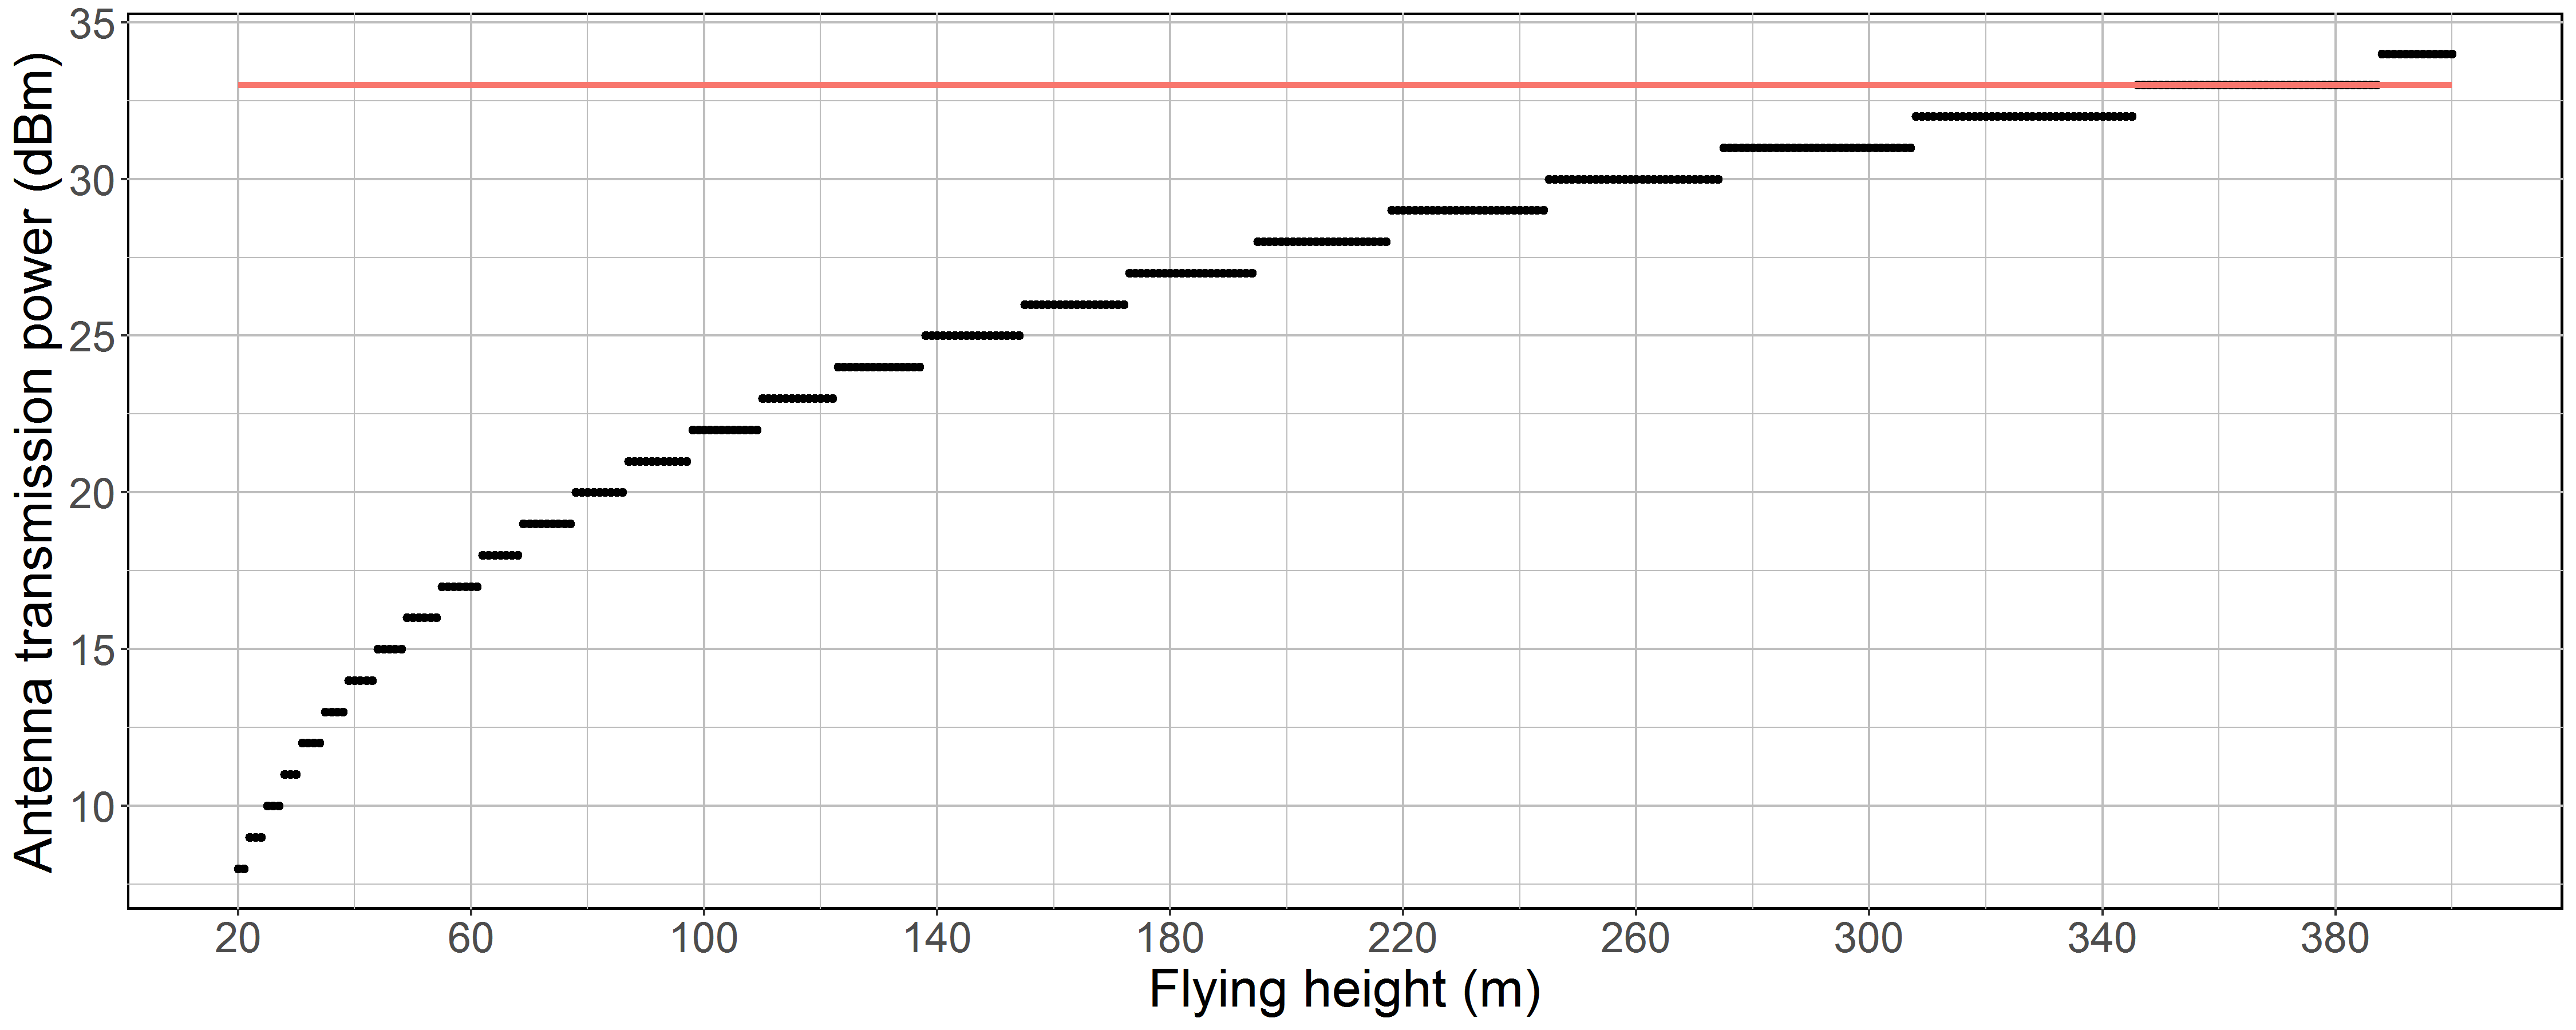
\includegraphics[width=\textwidth]{../results/s1/ptx.png}
  \caption{Minimal required transmission power by the antenna to reach the ground just below it. The red line shows the default maximum transmission power.}
  \label{fig:ptxfh}
\end{figure}

This scenario is investigated with a microstrip patch antenna using power consumption optimization. 
 However, the chosen optimization strategy does not really matter as already explained in  \ref{sec:scenarios_s1}. This is because the decision 
 algorithm decides which user 
needs to be connected to which \gls{UABS}. Since only one \gls{UABS} is available, both optimization strategies will behave identical.
Further, also the used antenna will not make any difference
despite the fact that a microstrip patch antenna has attenuation while an \gls{isotropicradiator} does not.
The user is namely positioned in the perfect center of the main beam where there is 
no attenuation experienced in either cases. So the results are applicable for the four possible cases from figure \ref{fig:fourCasesMatrix}.

\FloatBarrier
\subsection{Influence of the Flying Height}
\label{sub:senario1_influenceOfFlyHeight}

This subsection investigates how the flying height of a \gls{UABS} influences $SAR_{10g}$ and power consumption.
The $SAR_{10g}$, which is actually induced electromagnetic radiation into the user, is represented in figure \ref{fig:s1_fhsar}
and shows that for a low flying \gls{UAV}, \gls{DL} radiation is the main source of electromagnetic exposure.
This changes around an altitude of 80 metres where the \gls{UL} radiation from the \gls{UE}
exceeds the \gls{DL} radiation in order to still be able to reach the high flying \gls{UABS}s.

\gls{SAR}-values are caused by the transmitted power  $P_{tx}$ of the antenna. The $P_{tx}$ in section \ref{s1a}
showed a discontinue behaviour that sometimes radiates more than strictly necessary. This has thus a direct influence
on the \gls{DL} \gls{SAR}; hence, the same discontinue behaviour. The \gls{DL} \gls{SAR} can be simplified to a perfect constant line
at 10 $nW/kg$.
This constant behaviour can once again be explained with power control. When the \gls{UABS} flies lower, there is less path loss and the \gls{UABS} 
will therefore reduce the $P_{tx}$. 
We can therefore confirm that the electromagnetic exposure from the \gls{UABS} is a constant fraction of power and distance.
The electromagnetic radiation from the \gls{UE} shows in figure \ref{fig:s1_fhsar} an exponential behaviour. The power
used by the antenna is calculated with formula \ref{eq:powerUE}  and depends mainly on path loss.
\gls{UE} will, similar to \gls{UABS}s, radiate just enough so the \gls{SNR} is high enough to be decoded by the receiver.
The only difference with \gls{DL} radiation is that the distance between the radiator and the user remains unchanged. 
Therefore, the \gls{UL} electromagnetic radiation experienced by the user will increase when the flying altitude of the \gls{UABS} increases.
The \gls{UL} radiation starts very low with only $1\ nW/kg$ measured when the flying height is 20 metres. This increases fast to $66\ nW/kg$
at 200 metres.
%\begin{equation}
%\vec{E} (V/m) = \frac{\Delta U (V) }{\Delta x (m)}
%\label{eq:exposureBasicFormula}
%\end{equation}
%The SAR values are the result of multiplying the electromagnetic exposure with a constant as explained in equation \ref{eq:DLconvertion}. So both have a linear relationship.
Figure \ref{fig:s1_fhsar} does not show radiation from neighbours, because there are none present in this scenario. 
Finally, all these values are added up as explained in formula \ref{eq:overallSARwb} resulting in the total \gls{SAR}
to which our user is exposed, represented by the black line in \ref{fig:s1_fhsar}.

\begin{figure}[]
\centering
  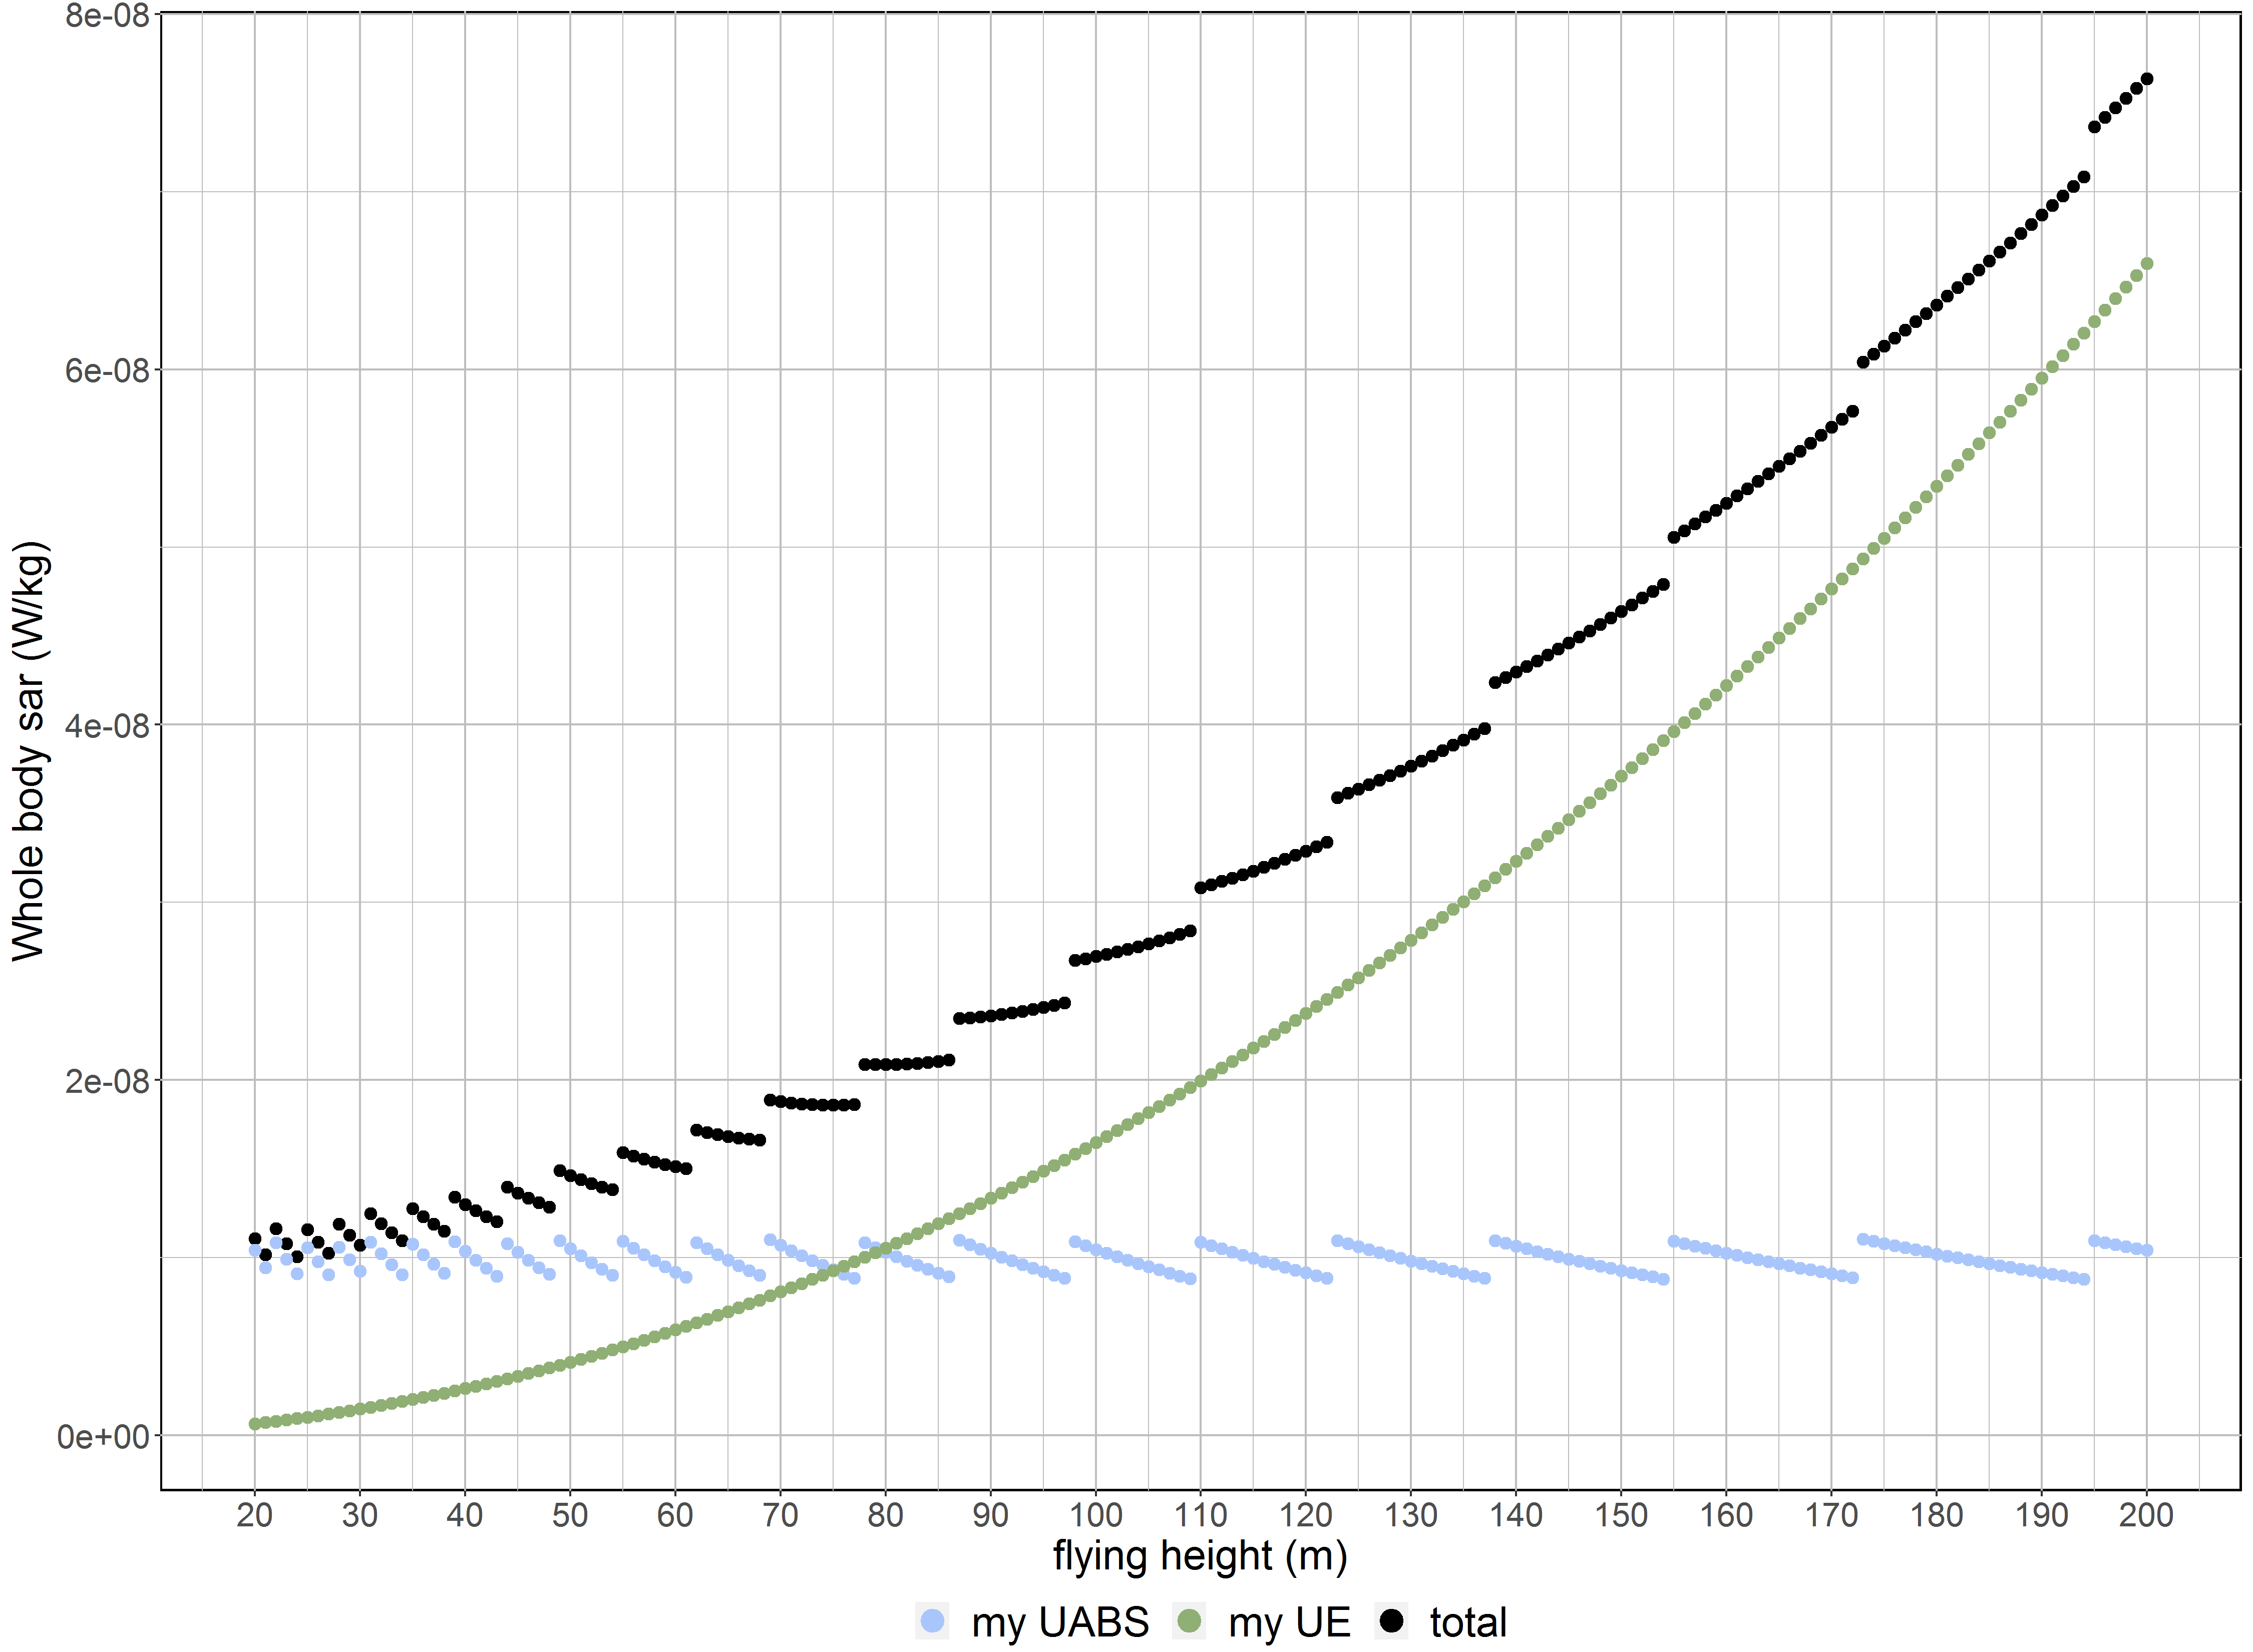
\includegraphics[width=\textwidth]{../results/s1/fhvssar.png}
  \caption{This figure shows how SAR values from different sources are influenced by different flying altitudes.}
  \label{fig:s1_fhsar}
\end{figure}

The power consumption of the entire network presented in figure \ref{fig:fhvspc} is here of course for the only \gls{UABS} available.
The energy is based on the transmission power of the antenna and the used battery by the \gls{UAV}.
Section \ref{s1a} already explained the reason behind the stepped function. The transmission power 
is an important parameter when calculating the used power and is the cause that we see the same stepped behaviour in 
figure \ref{fig:fhvspc}. All individual results (indicated with dots) can once again be simplified 
with a connected line that clearly shows an exponentially behaviour. The grey shadow 
behind the line represented the confidence interval.

\begin{figure}[t]
  \centering
  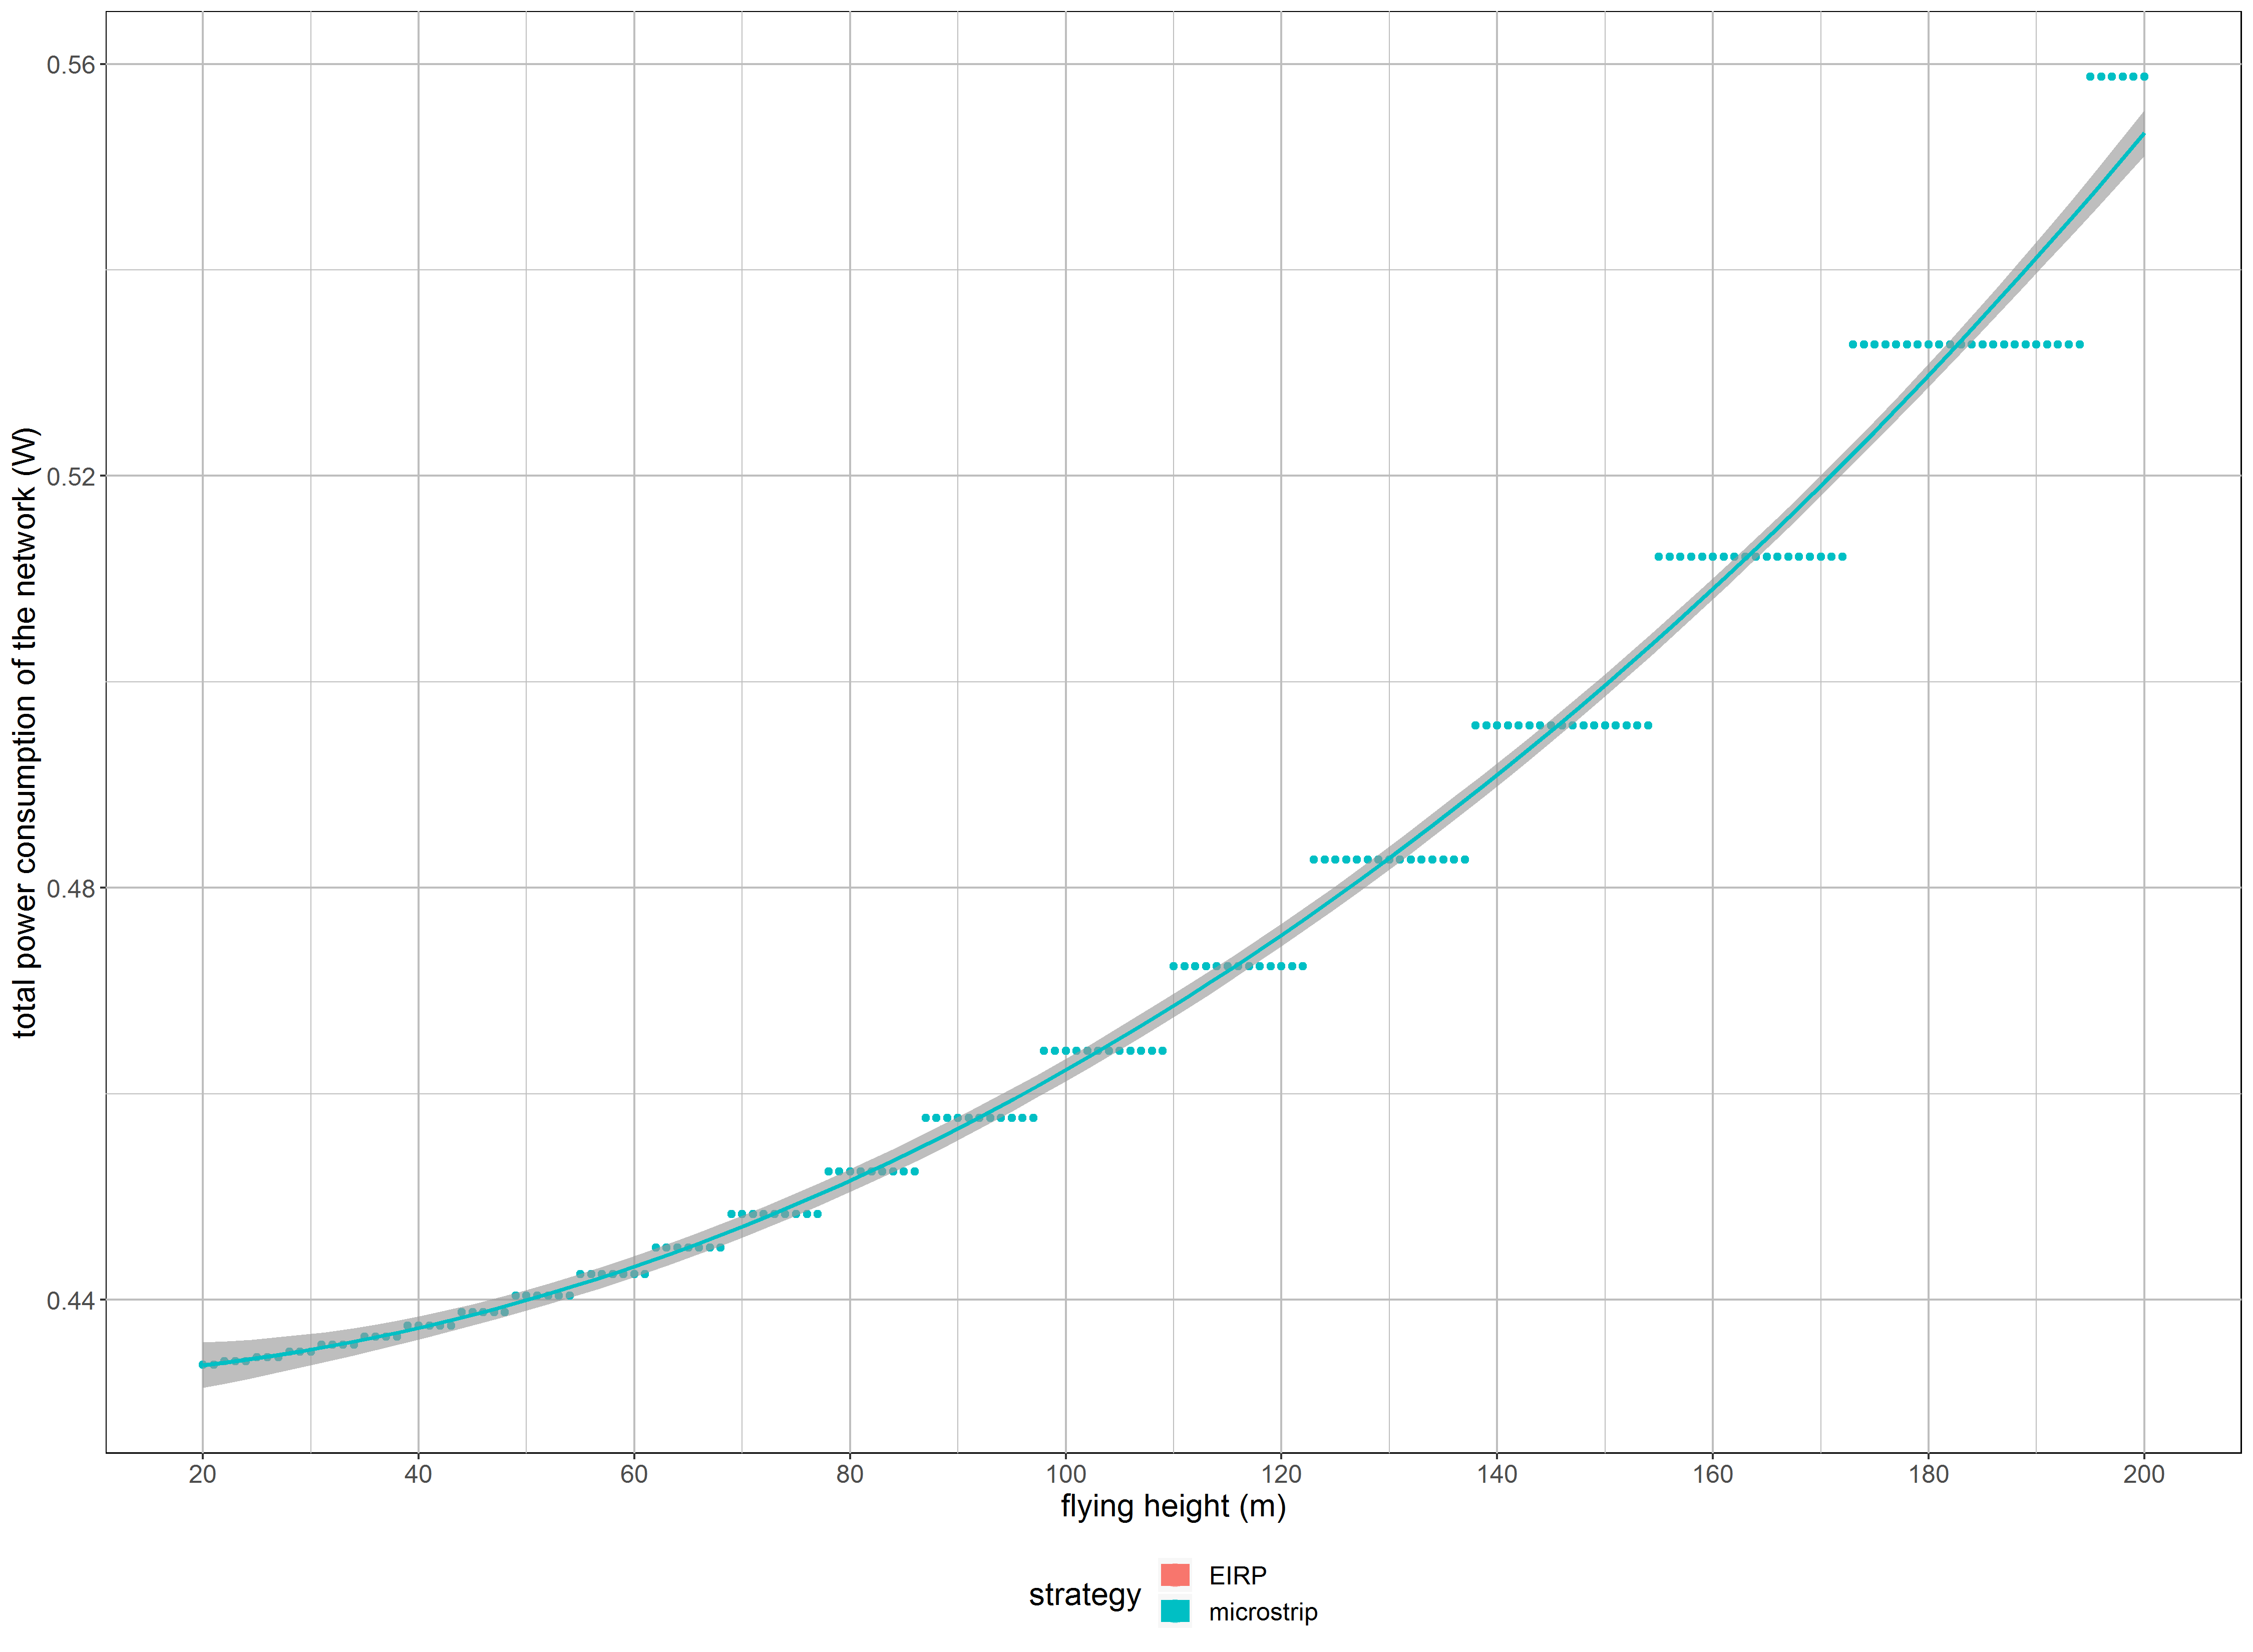
\includegraphics[width=\textwidth]{../results/s1/fhvspc.png}
  \caption{This figure shows the behaviour of the power consumption over the entire network at different flying  heights.
  For this scenario, the power is used by only one \acs{UABS}.}
  \label{fig:fhvspc}
\end{figure}
%%%%%%%%%%%%%%%%%%%%%%%%%%%%%%%%%%%%%%%%%%%%%%%%%%%%%%%%%%%%%%%%%%%%%%%%%%%%%%%%%%%%%%%%%%%%%%%%%%%%%%%%%%%%%
\FloatBarrier
\section{Scenario II: Increased Population}

This scenario has just like the previous scenario only one \gls{UAV} available. However, more users will be present in the network.
First, a variable flying altitude is investigated for a fixed number of 224 users. 
Secondly, the flying height is set to 100 metres with a variable number of users.
When designing the network, there will be as much possible \gls{UAV} locations as there are users in the network and the tool
will consider all of them. Only when the program is finished, one \gls{UAV} will remain.
Each considered input value will be averaged over 20 simulations.



\subsection{Influence of the Flying Altitude}
The first evaluated parameter of this scenario investigates how the network, consisting out of one \acs{UABS}, behaves when applied on an ordinary day during rush hours. 
Different fixed flying heights are considered while 224 active users are distributed uniformly over the city centre of Ghent. 
as presented in the example of figure \ref{fig:s2a:distribution}.
\begin{figure}[h]
  \centering
  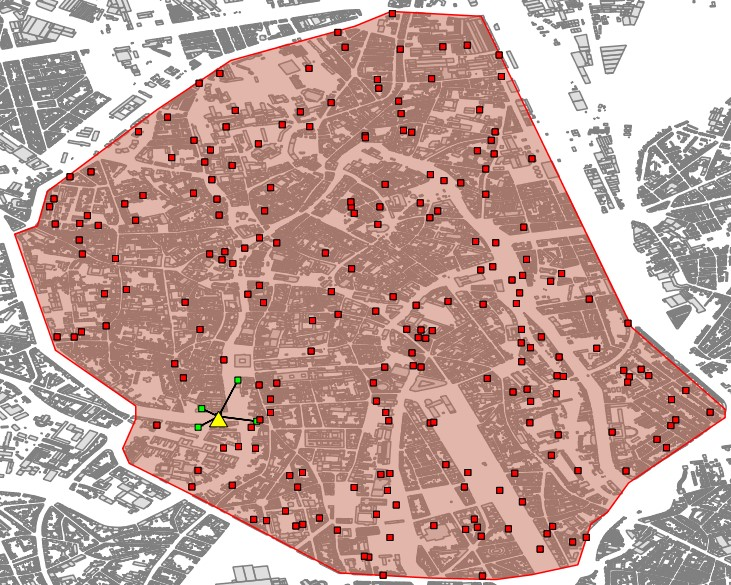
\includegraphics[width=0.6\textwidth]{../images/ghentDistribution_pcEIRP_1drone.jpg}
  \caption{Example of an EIRP \gls{PwrC Opt} network with only one \acs{UABS} (yellow triangle). Only a very few users (green) are connected.
  All other users (red) remain uncovered.}
  \label{fig:s2a:distribution}
\end{figure}

Figure \ref{fig:s2a_dlAndPc} presents the average \gls{DL} exposure and average total power consumption. The grey area indicates the confidence interval. 
A power consumption optimized network with an \gls{EIRP} antenna (green) has the highest exposure during the 
entire experiment. At the default flying height of 100 metres, an electromagnetic field radiation 
of 10 $mV/m$ is measured.
This is logical when comparing to an EIRP antenna in an exposure optimized network (red) with only $8.5\ mV/m$. 
However, when looking at figure \ref{fig:s2a_dlAndPc}.b, the power consumption in a power consumption optimized network is not necessarily less 
than in an exposure optimized network. 
For example, an \gls{EIRP} and microstrip antenna will require at the default flying height respectively
20 $mW$ and 10 $mW$ more in a power consumption optimized network than in an exposure optimized network.
To understand this, the behaviour of the deployment tool needs to be understood first. 
A power consumption optimized network will result in a few high powered \gls{UABS}s because increasing the input power of an antenna costs 
less than activating a new  \gls{UAV}. Likewise, an exposure optimized network 
generates a lot of low powered \gls{UABS}s because the lower the power of the antenna, the lower the exposure. This has the consequence that the cover radius 
is less and therefore requires more \gls{UAV}s which costs more energy.
When only a limited amount of \gls{UABS}s are available, 
like only one in this scenario, the tool will only keep those \gls{UABS}s that cover the most users. 
Therefore, the power consumption in a power consumption optimized network is often higher. 

Figure \ref{fig:s2a_dlAndPc} further also shows how the electromagnetic radiation from the \gls{UABS}
starts  decreasing again at high altitude. A microstrip \gls{PwrC Opt} network is at his highest point  
around 162 metres and an \gls{EIRP} \gls{PwrC Opt} is at his highest at 195 metres.
This decline starts later for exposure optimized networks and is situated outside the investigated flying range.
The decreasing electromagnetic radiation at high flying altitudes is not caused by the obstructing buildings but by the 
distance in general.


\begin{figure}[h!]
  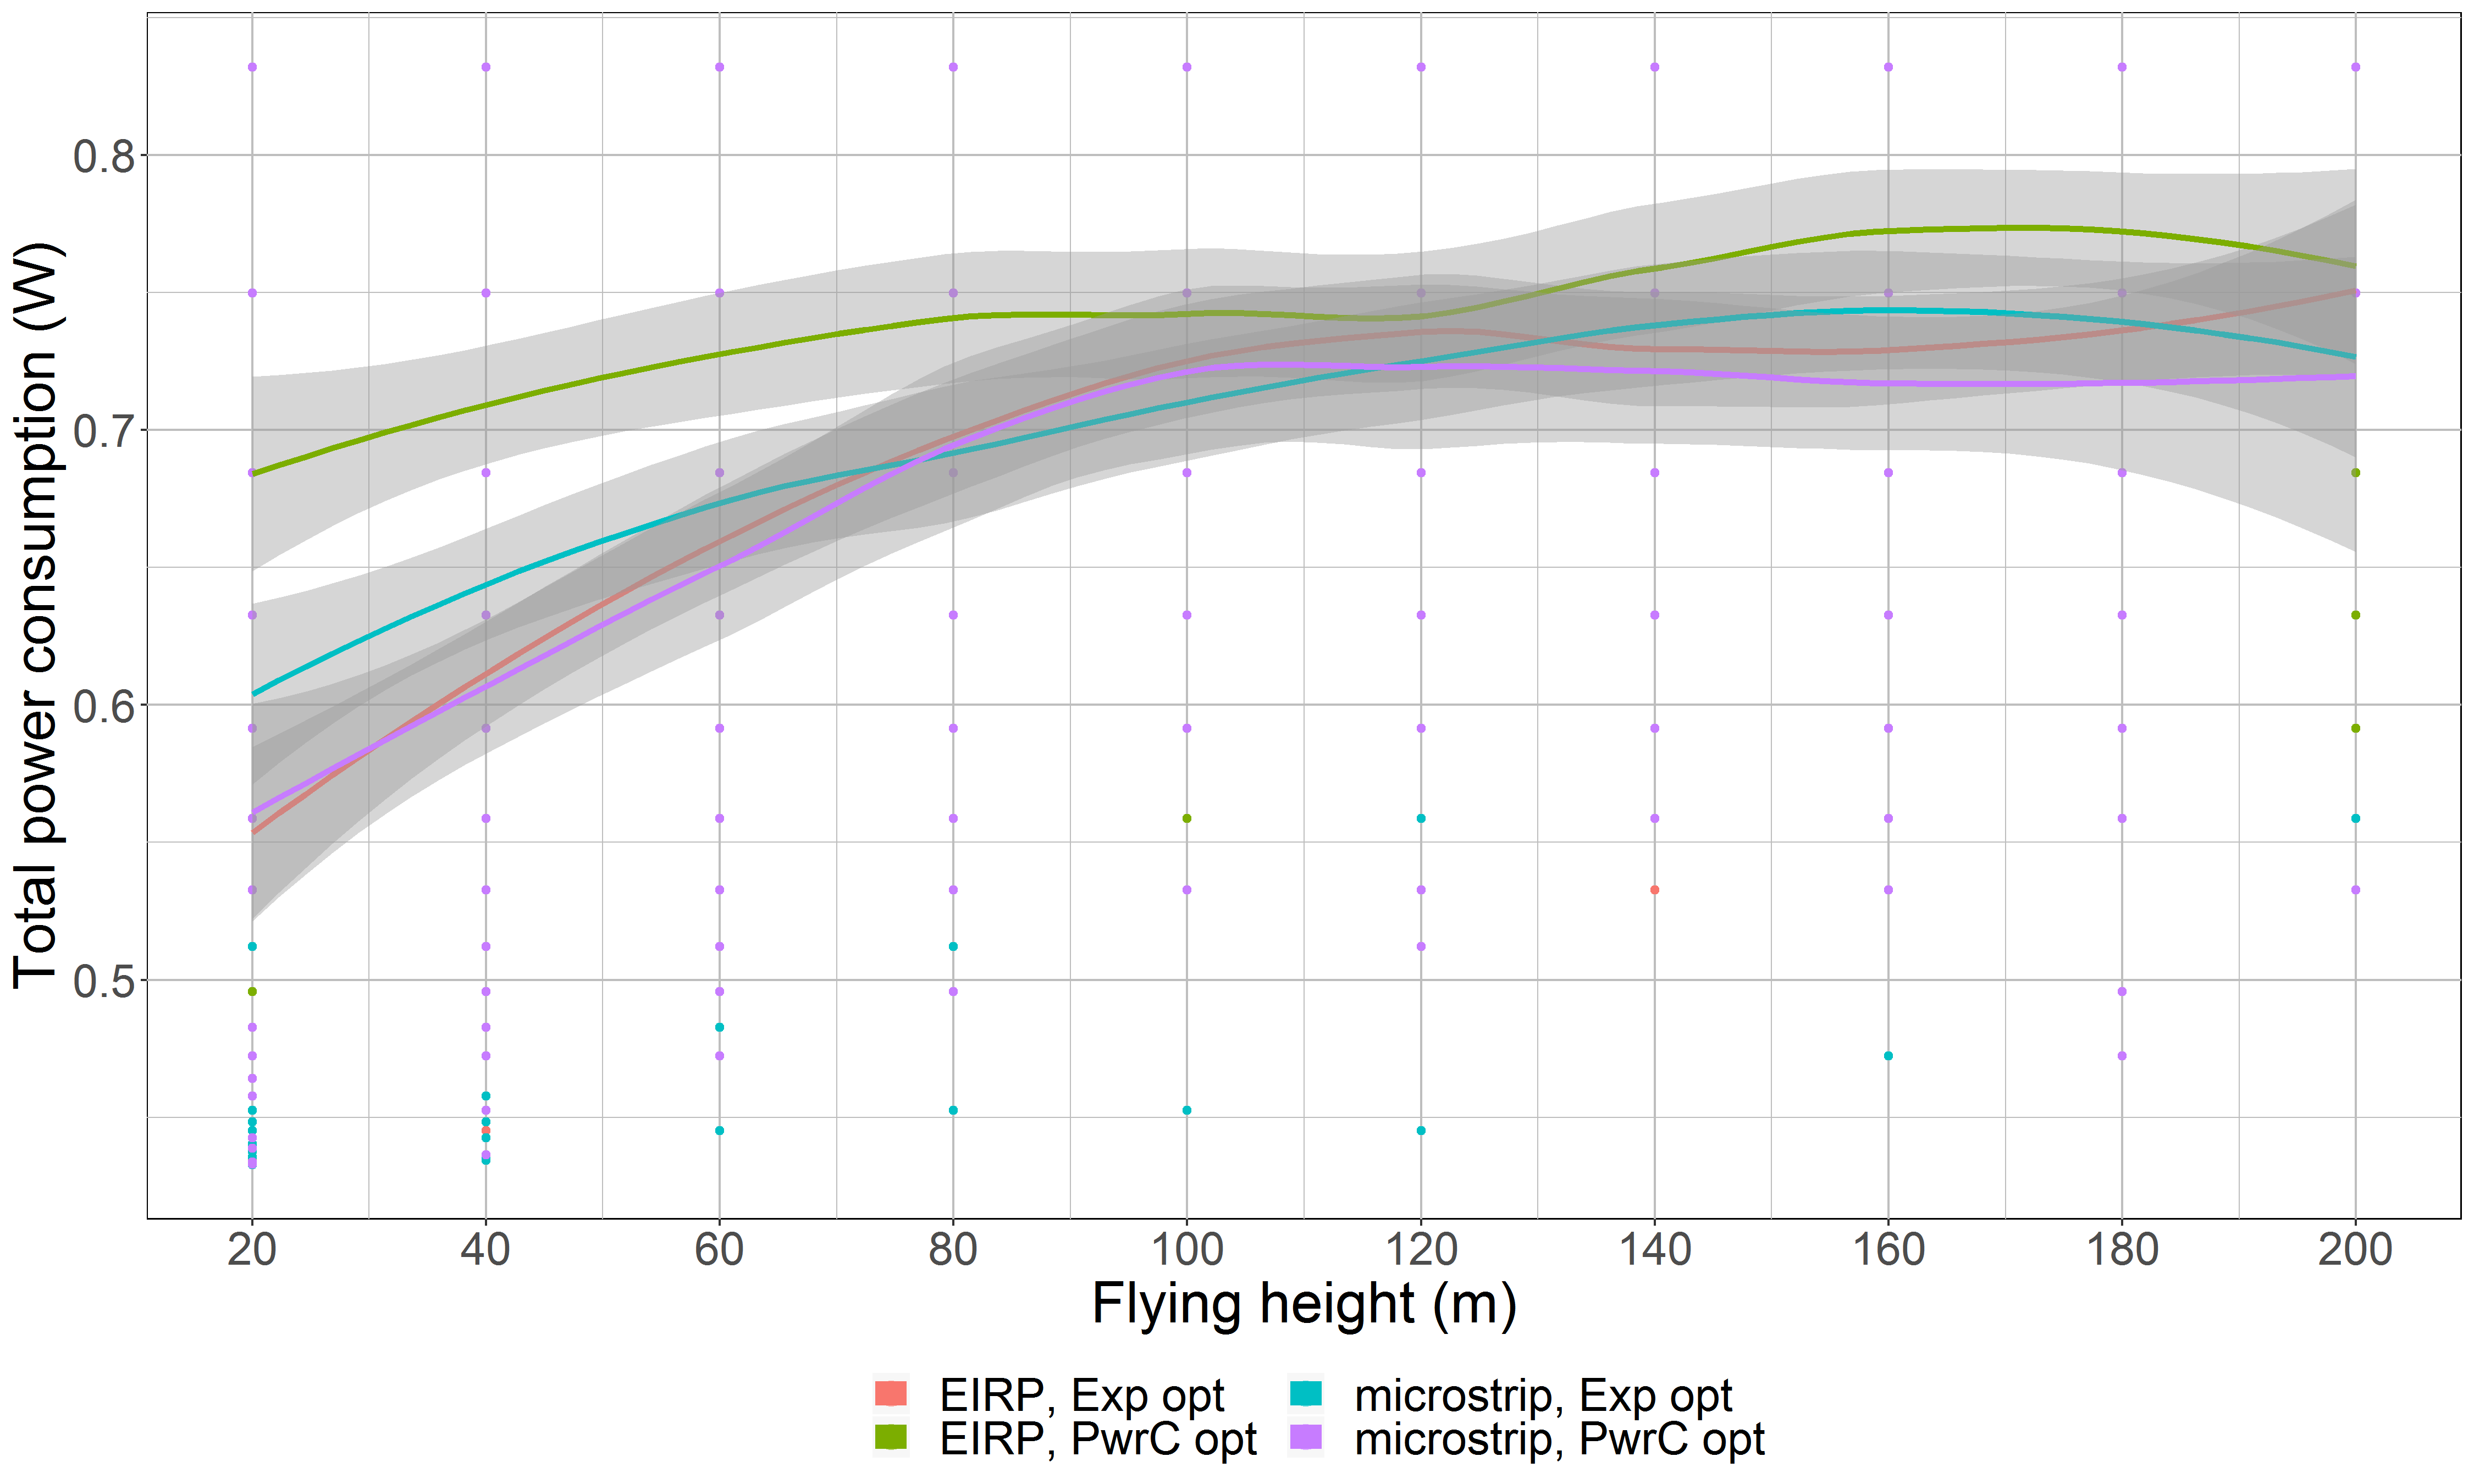
\includegraphics[width=\textwidth]{../results/s2/fhvsdlAndPc.png}
  \caption{Fig. (a) show how the flying height influences the downlink electromagnetic radiation of the average user and fig. (b) the
  power consumption of the entire network for the only \acs{UABS} available in the network.}
  \label{fig:s2a_dlAndPc}
\end{figure}

\FloatBarrier
\begin{wrapfigure}{r}{0.45\textwidth}
\vspace{-0.7cm}
  \begin{center}
    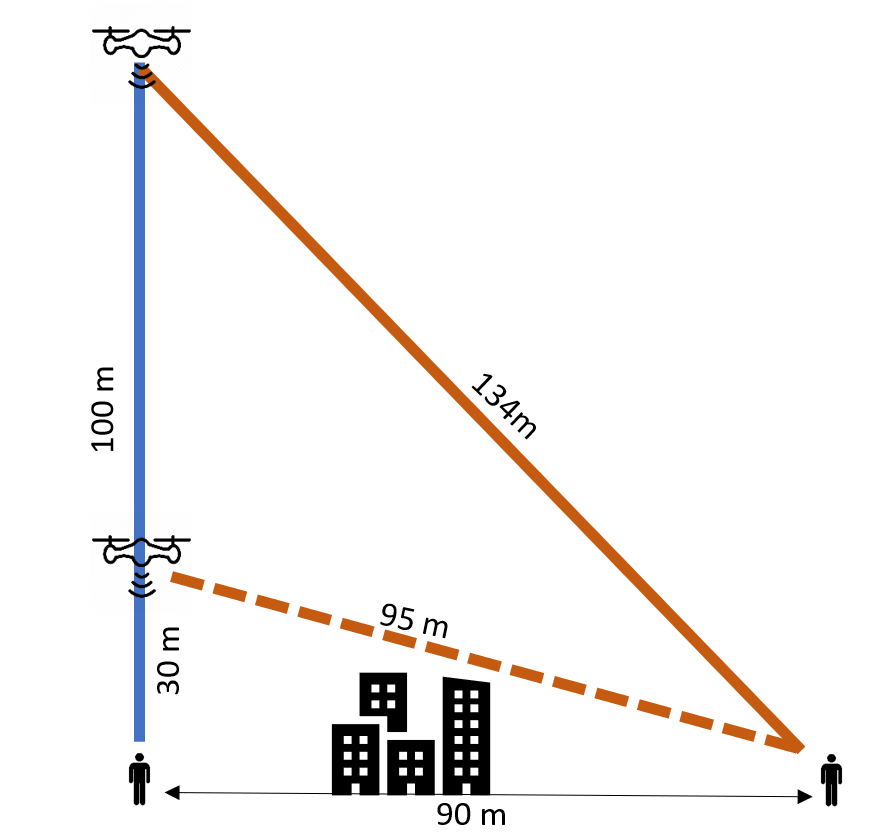
\includegraphics[width=0.45\textwidth]{../results/s2/proveScenario.png}
  \end{center}
  \caption{Schematic overview of Scenario II with only 2 users.}
  \label{fig:schematicprove}
\end{wrapfigure}

The \gls{DL} exposure in figure \ref{fig:s2a_dlAndPc} increases along with the flying height. One might expect a more constant 
behaviour like it was the case in figure \ref{fig:s1_fhsar} of Scenario I. To understand this, the scenario has been reduced  
to only two users and is illustrated in figure \ref{fig:schematicprove}.
The two users, who will be referred to by `red' and `blue', are 90 metres separated from each other with a building between them.
Scenario I already explained that the charts can be simplified and the blue line from fig. \ref{fig:prove} remains in fact constant between zero and 130 metres.
The chart shows that the \gls{UABS} is positioned above the blue user. The red user is in \gls{NLOS} as long as the \gls{UABS} remains below 20 metres.

Once the \gls{UABS} increases its flying altitude, the red user comes into \gls{LOS} but still remains uncovered. This is because the tool initially locates a possible 
\gls{UABS} above each user and thereafter performs the  fitness function. The applied fitness function must have decided that it is better to connect 
each user to the \gls{UABS} above him. In a final stage, the tool checks whether the number of online \gls{UAV}s does not exceed the capacity of the facility
which is here the case. The tool therefore deactivates one \gls{UABS} causing the red user to be uncovered. One could argue that the 
the red user should be connected to the online \gls{UAV} who is only 90 metres away. This would however require the online \gls{UAV} to increase its power consumption which 
would make the decisions made by the optimization strategy obsolete.
When the \gls{UAV} flies higher, the difference in distance between both users and the base station decreases. In other words, the Pythagorean theorem shows that when the flying height of the 
\gls{UABS} increases, the distance to the blue user increases faster compared to the distance between that same \gls{UABS} and the red user. This is also illustrated in 
figure \ref{fig:schematicprove}.
At 130 metres, the tool decides to connect both users to the same \gls{UABS}. Therefore, it increases its power consumption whereby the red user would  have the minimal 
required electromagnetic exposure. This has of course a negative influence on the blue user who is much more closer and experiences now a much higher exposure level in fig \ref{fig:prove}.
Around 180 metres, the  red and blue line switch because the \gls{UAV} changes position. As explained before, the tool assigns two possible \gls{UAV}s, one above 
each user. The tool must have decided that connecting both users to the other \gls{UAV}s improves the fitness function of the entire network even though that difference might be 
very little.
Finally, this brings us back to the weighted average exposure from figure \ref{fig:s2a_dlAndPc} where 223 users will behave like the  red user and only
one user behaves like the blue one. 
The red line therefore dominates the average exposure in figure \ref{fig:s2a_dlAndPc}.

\begin{figure}[h!]
  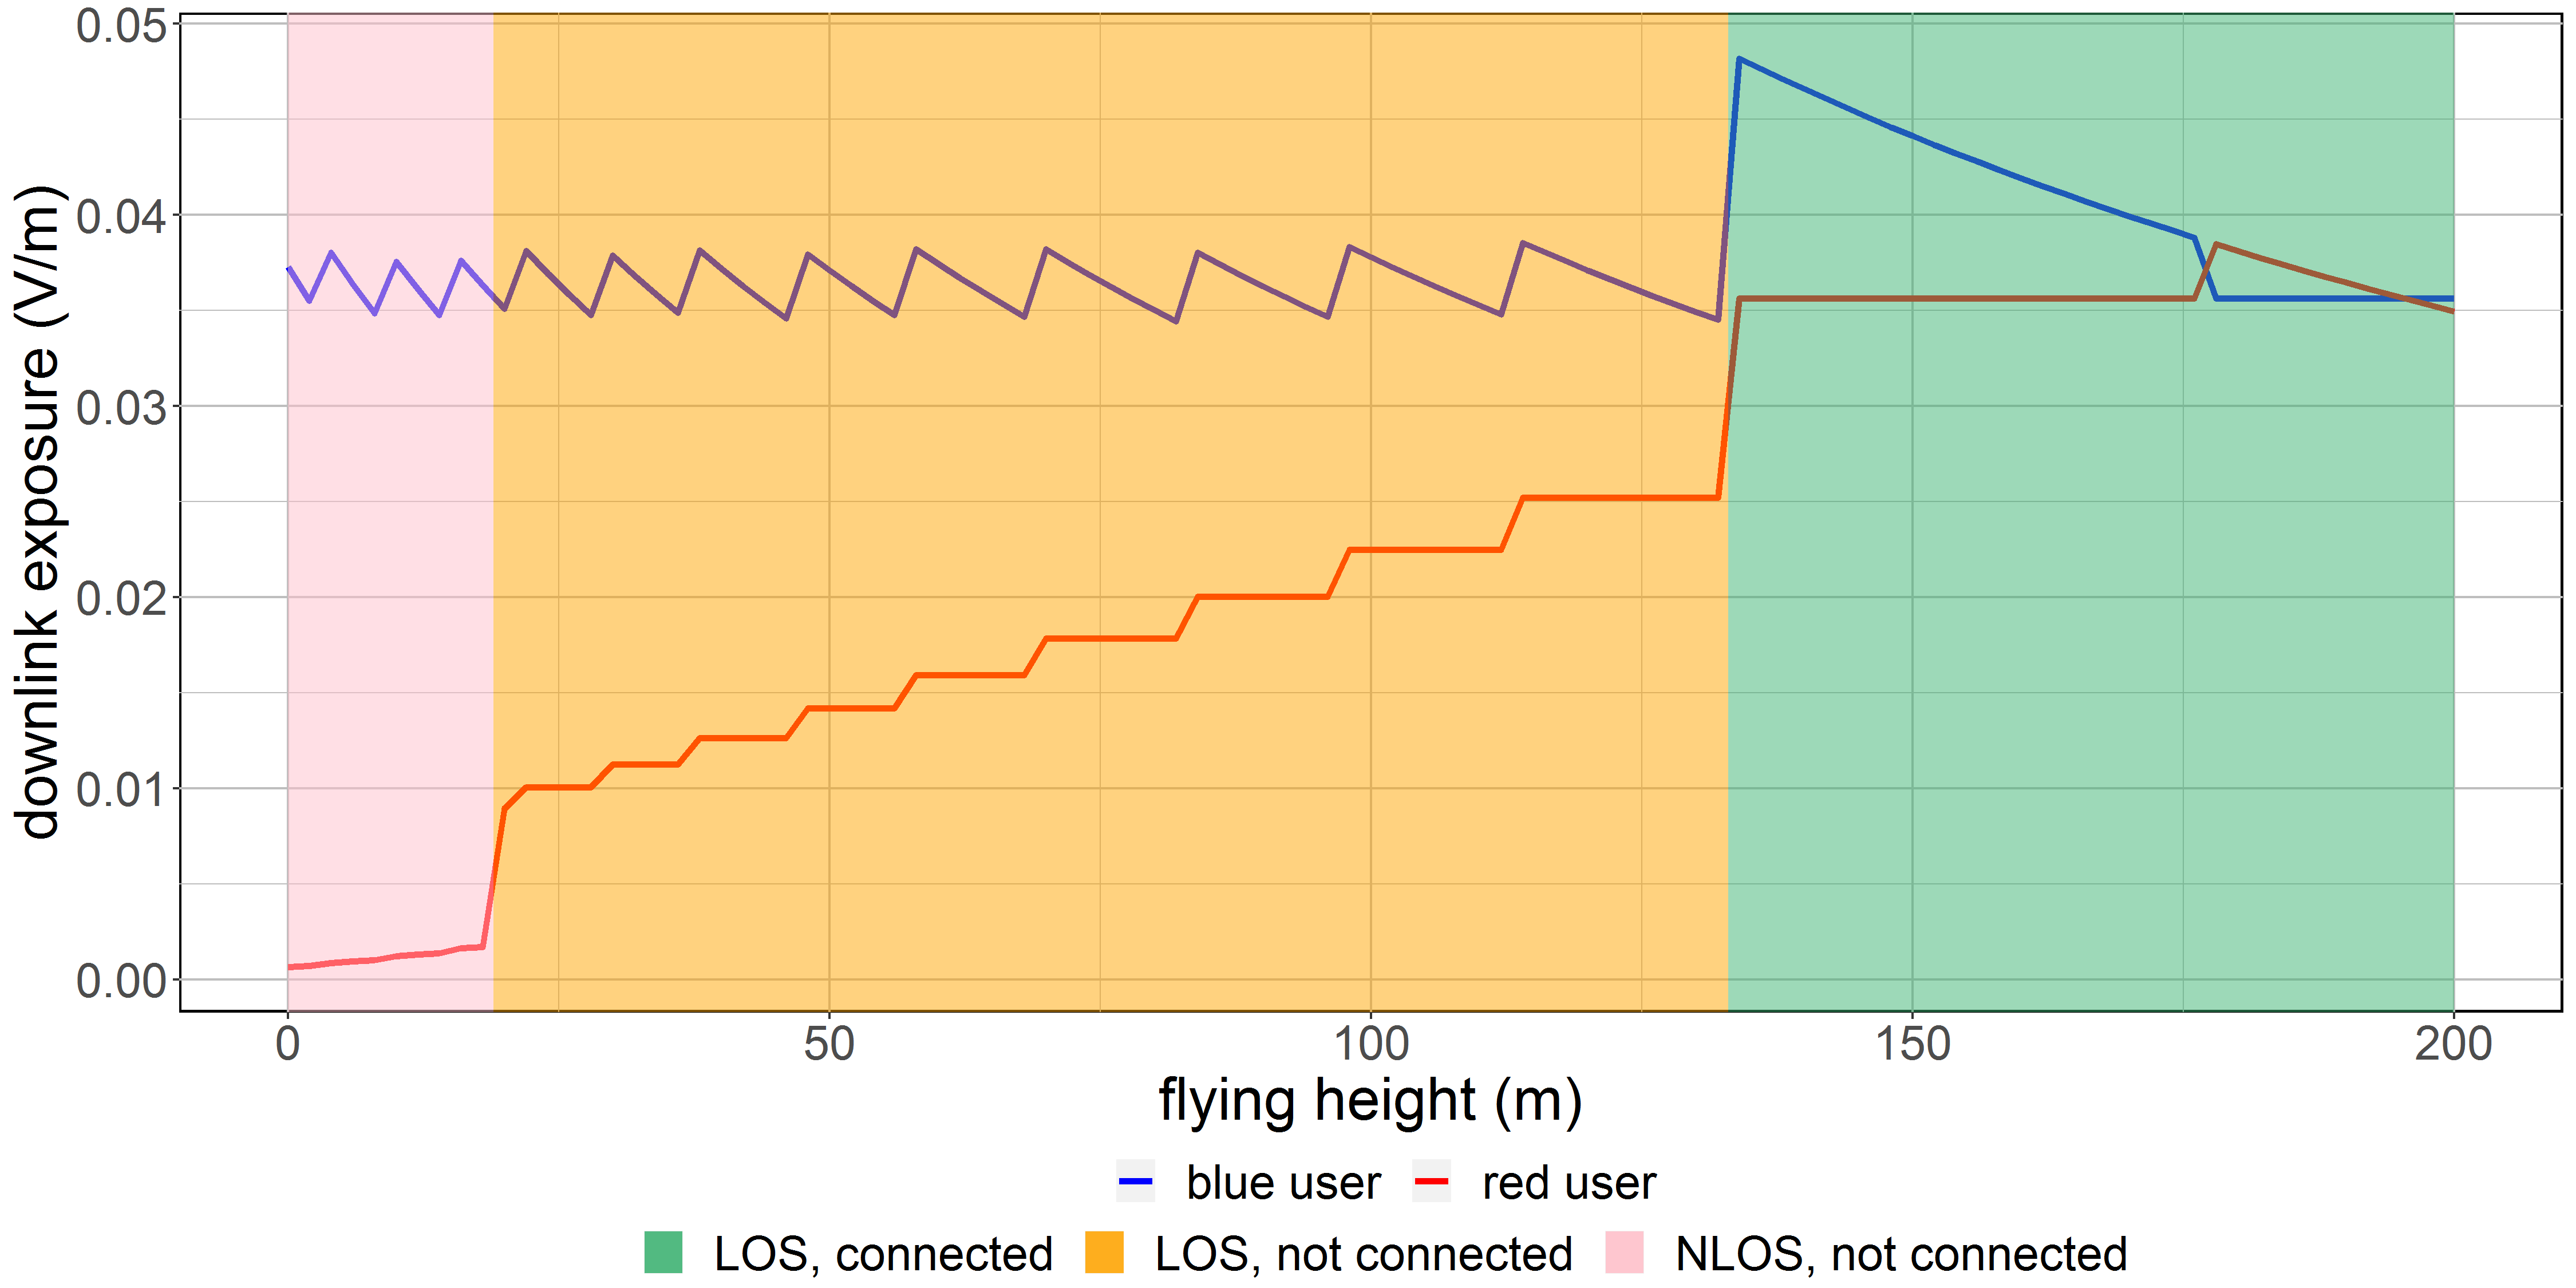
\includegraphics[width=\textwidth]{../results/s2/prove.png}
  \caption{Scenario II with only 2 users. The coloured areas are only applicable for the red user. 
  The blue user is connected during the entire time.}
  \label{fig:prove}
\end{figure}


Figure \ref{fig:s2a_dlAndPc} showed that the electromagnetic exposure of the average user increases along with the flying height
which reflects itself on better coverage as visible in figure  \ref{fig:s2fhvscov}.
Increasing the flying height from 20 to 100 metres improves the coverage between 1\% and 2\% for all four configurations.
When replacing the fictional \gls{EIRP} antenna by a microstrip patch antenna, the percentage of covered users drops for both 
optimization strategies less than 1\%. 
The difference is caused by users who have a higher horizontal distance between themselves and the \gls{UABS}. Microstrip 
patch antennae have a smaller aperture angle than an \gls{isotropicradiator} and have therefore a smaller range.
When a microstrip patch antenna is positioned higher, the range of the antenna increases 
since the angle between the user and the \gls{UABS}'s main lob decreases. The user will therefore experience less attenuation.

\begin{figure}[h!]
  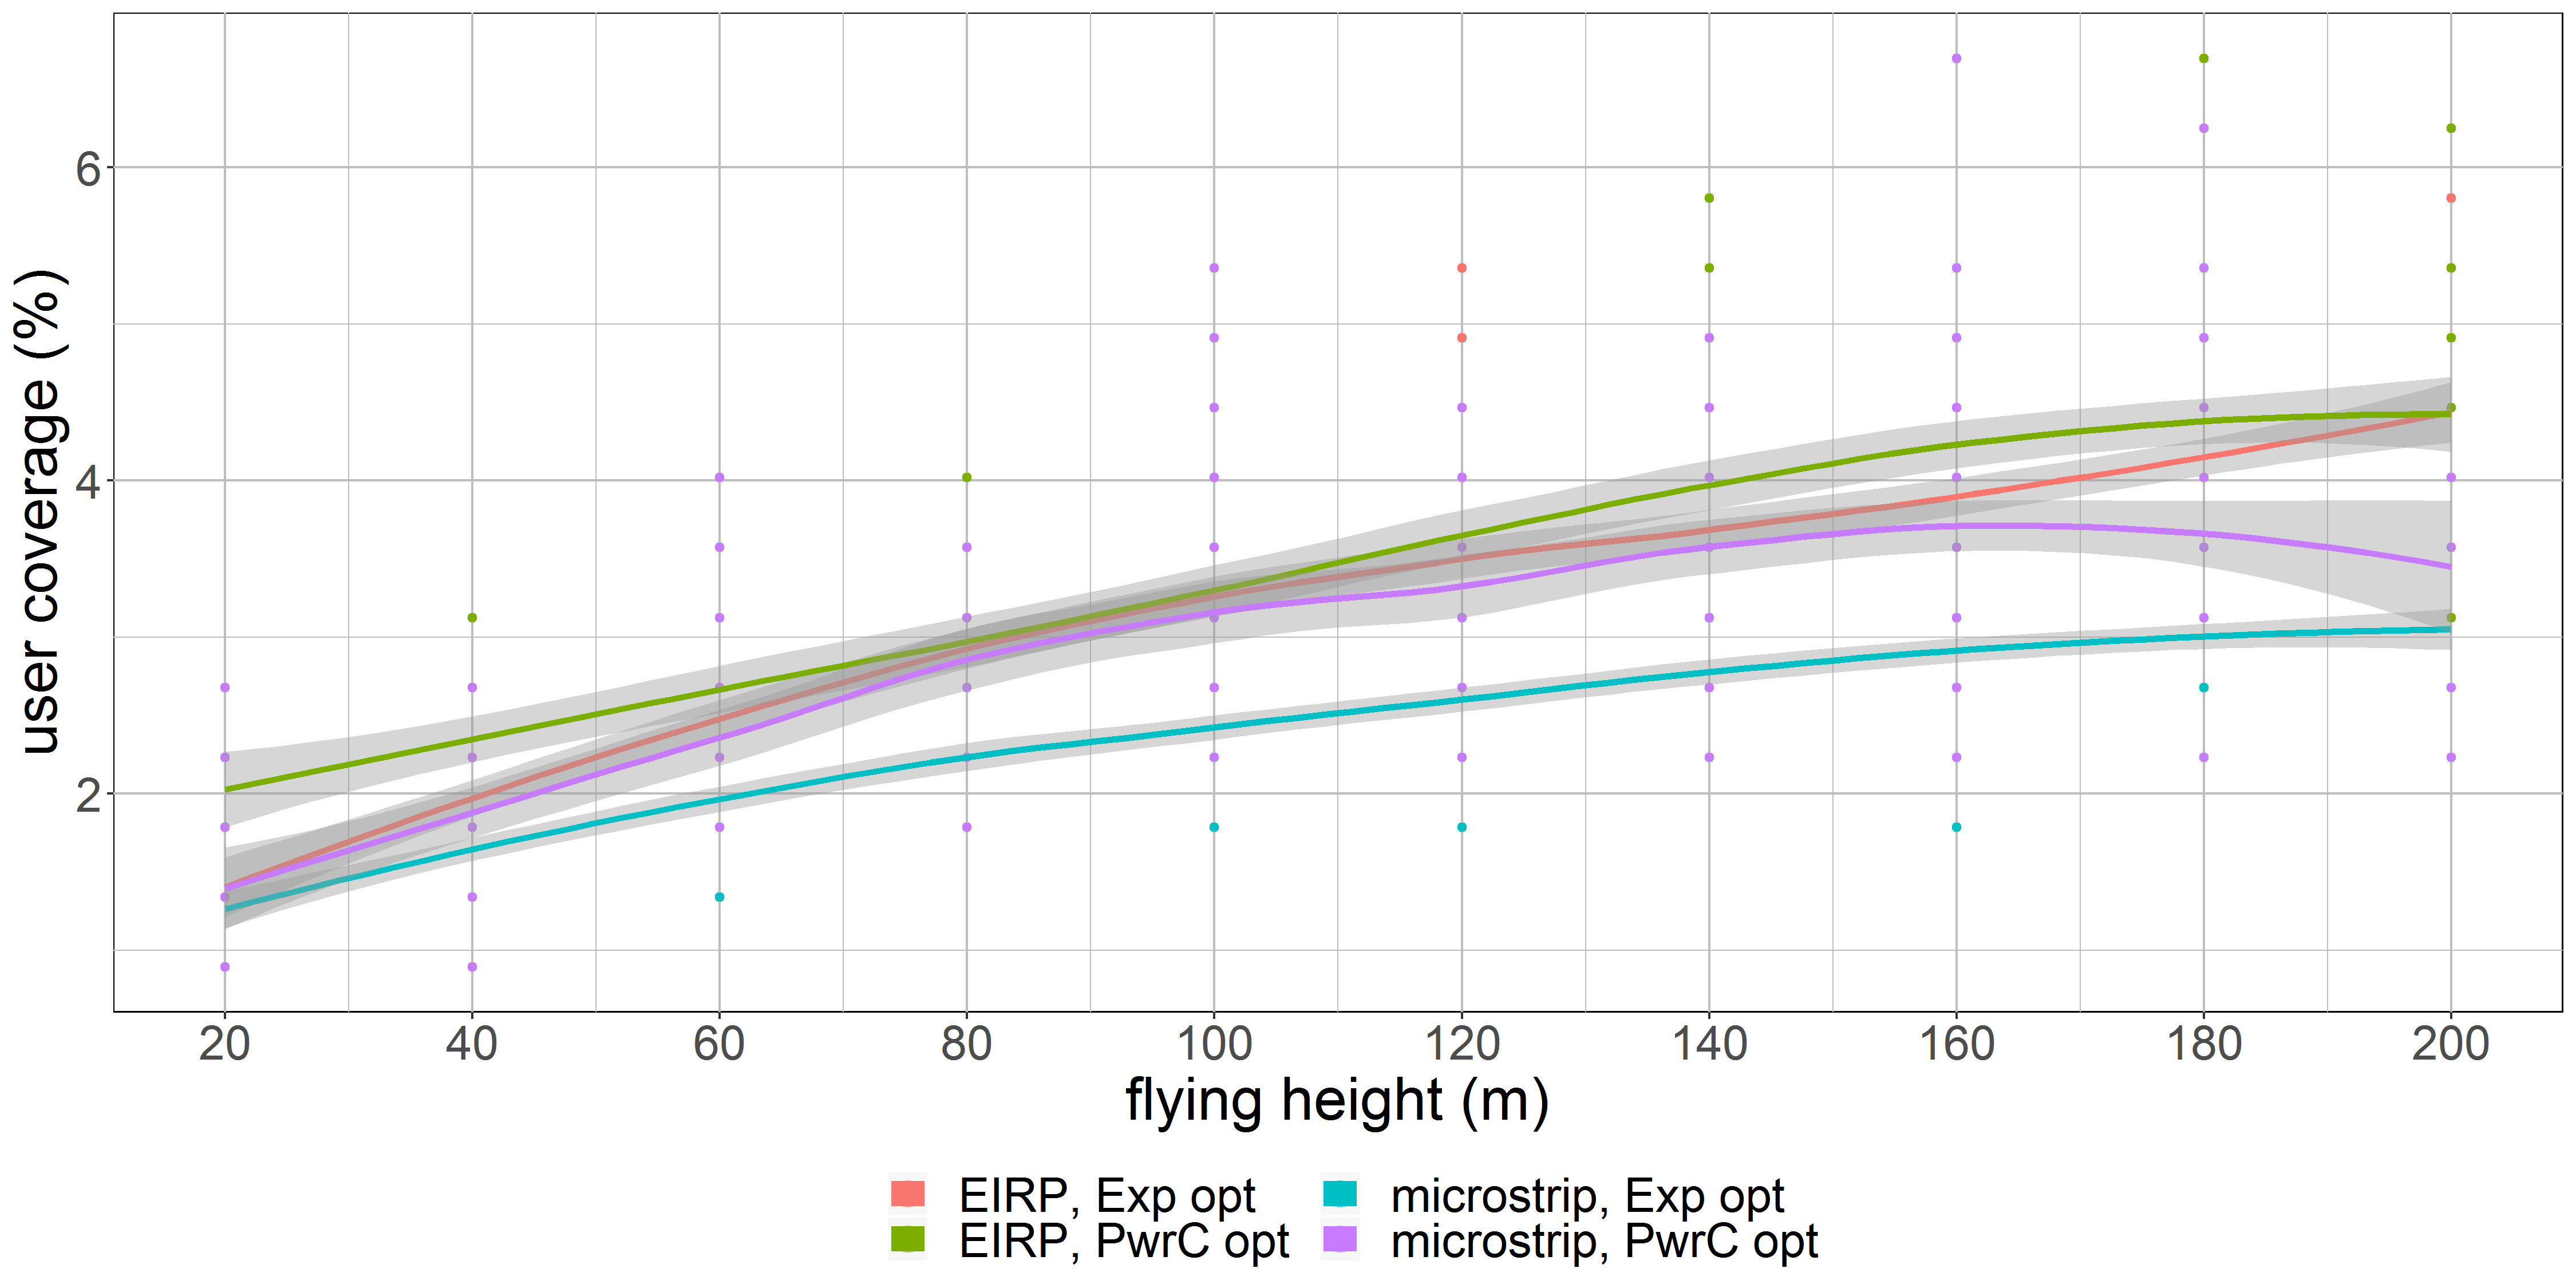
\includegraphics[width=\textwidth]{../results/s2/fhvscov.png}
  \caption{This graph shows the percentage of covered users for only one \acs{UABS} at different flying heights.}
  \label{fig:s2fhvscov}
\end{figure}

Eventually, figure \ref{fig:s2shfourSourcesMatrix} shows the whole body $SAR_{10g}$ for the weighted average user, deducted from all electromagnetic sources. 
This combines the exposure 
of the only \gls{UABS} available in the network, 
the \gls{UL} exposure from the user’s own device and the exposure of the devices from all other covered users. 
When investigating the three different sources, we see 
that the $SAR^{myUABS}$ shows the same curve as it did with the electromagnetic exposure 
in figure \ref{fig:s2a_dlAndPc}.a. This is normal behaviour considering that equation \ref{eq:DLconvertion} is able of 
converting the \gls{DL} exposure to \gls{SAR} by simply multiplying with a constant.
During the entire time is $SAR^{myUABS}$ the most dominant factor followed by 
 the near-field radiation from the user's own device.
The far-field radiation from other \gls{UE} barely has influence. 
As an illustration, when the \gls{UABS} flies at 140 metres, the average user in an \gls{EIRP} \gls{PwrC Opt} network will 
experience around  2.1 $nW/kg$ from the \gls{UABS} and around 0.2 $nW/kg$ from his own device.
The exposure from other \gls{UE} can be neglected with 0.03 $pW/kg$. A low but plausible value considering that most 
\gls{UE} are not radiating anything since they are uncovered (hence the many red dots in fig. \ref{fig:s2a:distribution}).

The weighted average $SAR^{ul}_{10g}$ from the own device is zero in an exposure optimized network with a microstrip patch antenna 
which is even lower than the $SAR^{neighbours}_{10g}$.
This is because the coverage in this scenario is so low that the weighted average 
only consists of uncovered users and the transmission power of an uncovered user is zero.

\begin{figure}[h!]
  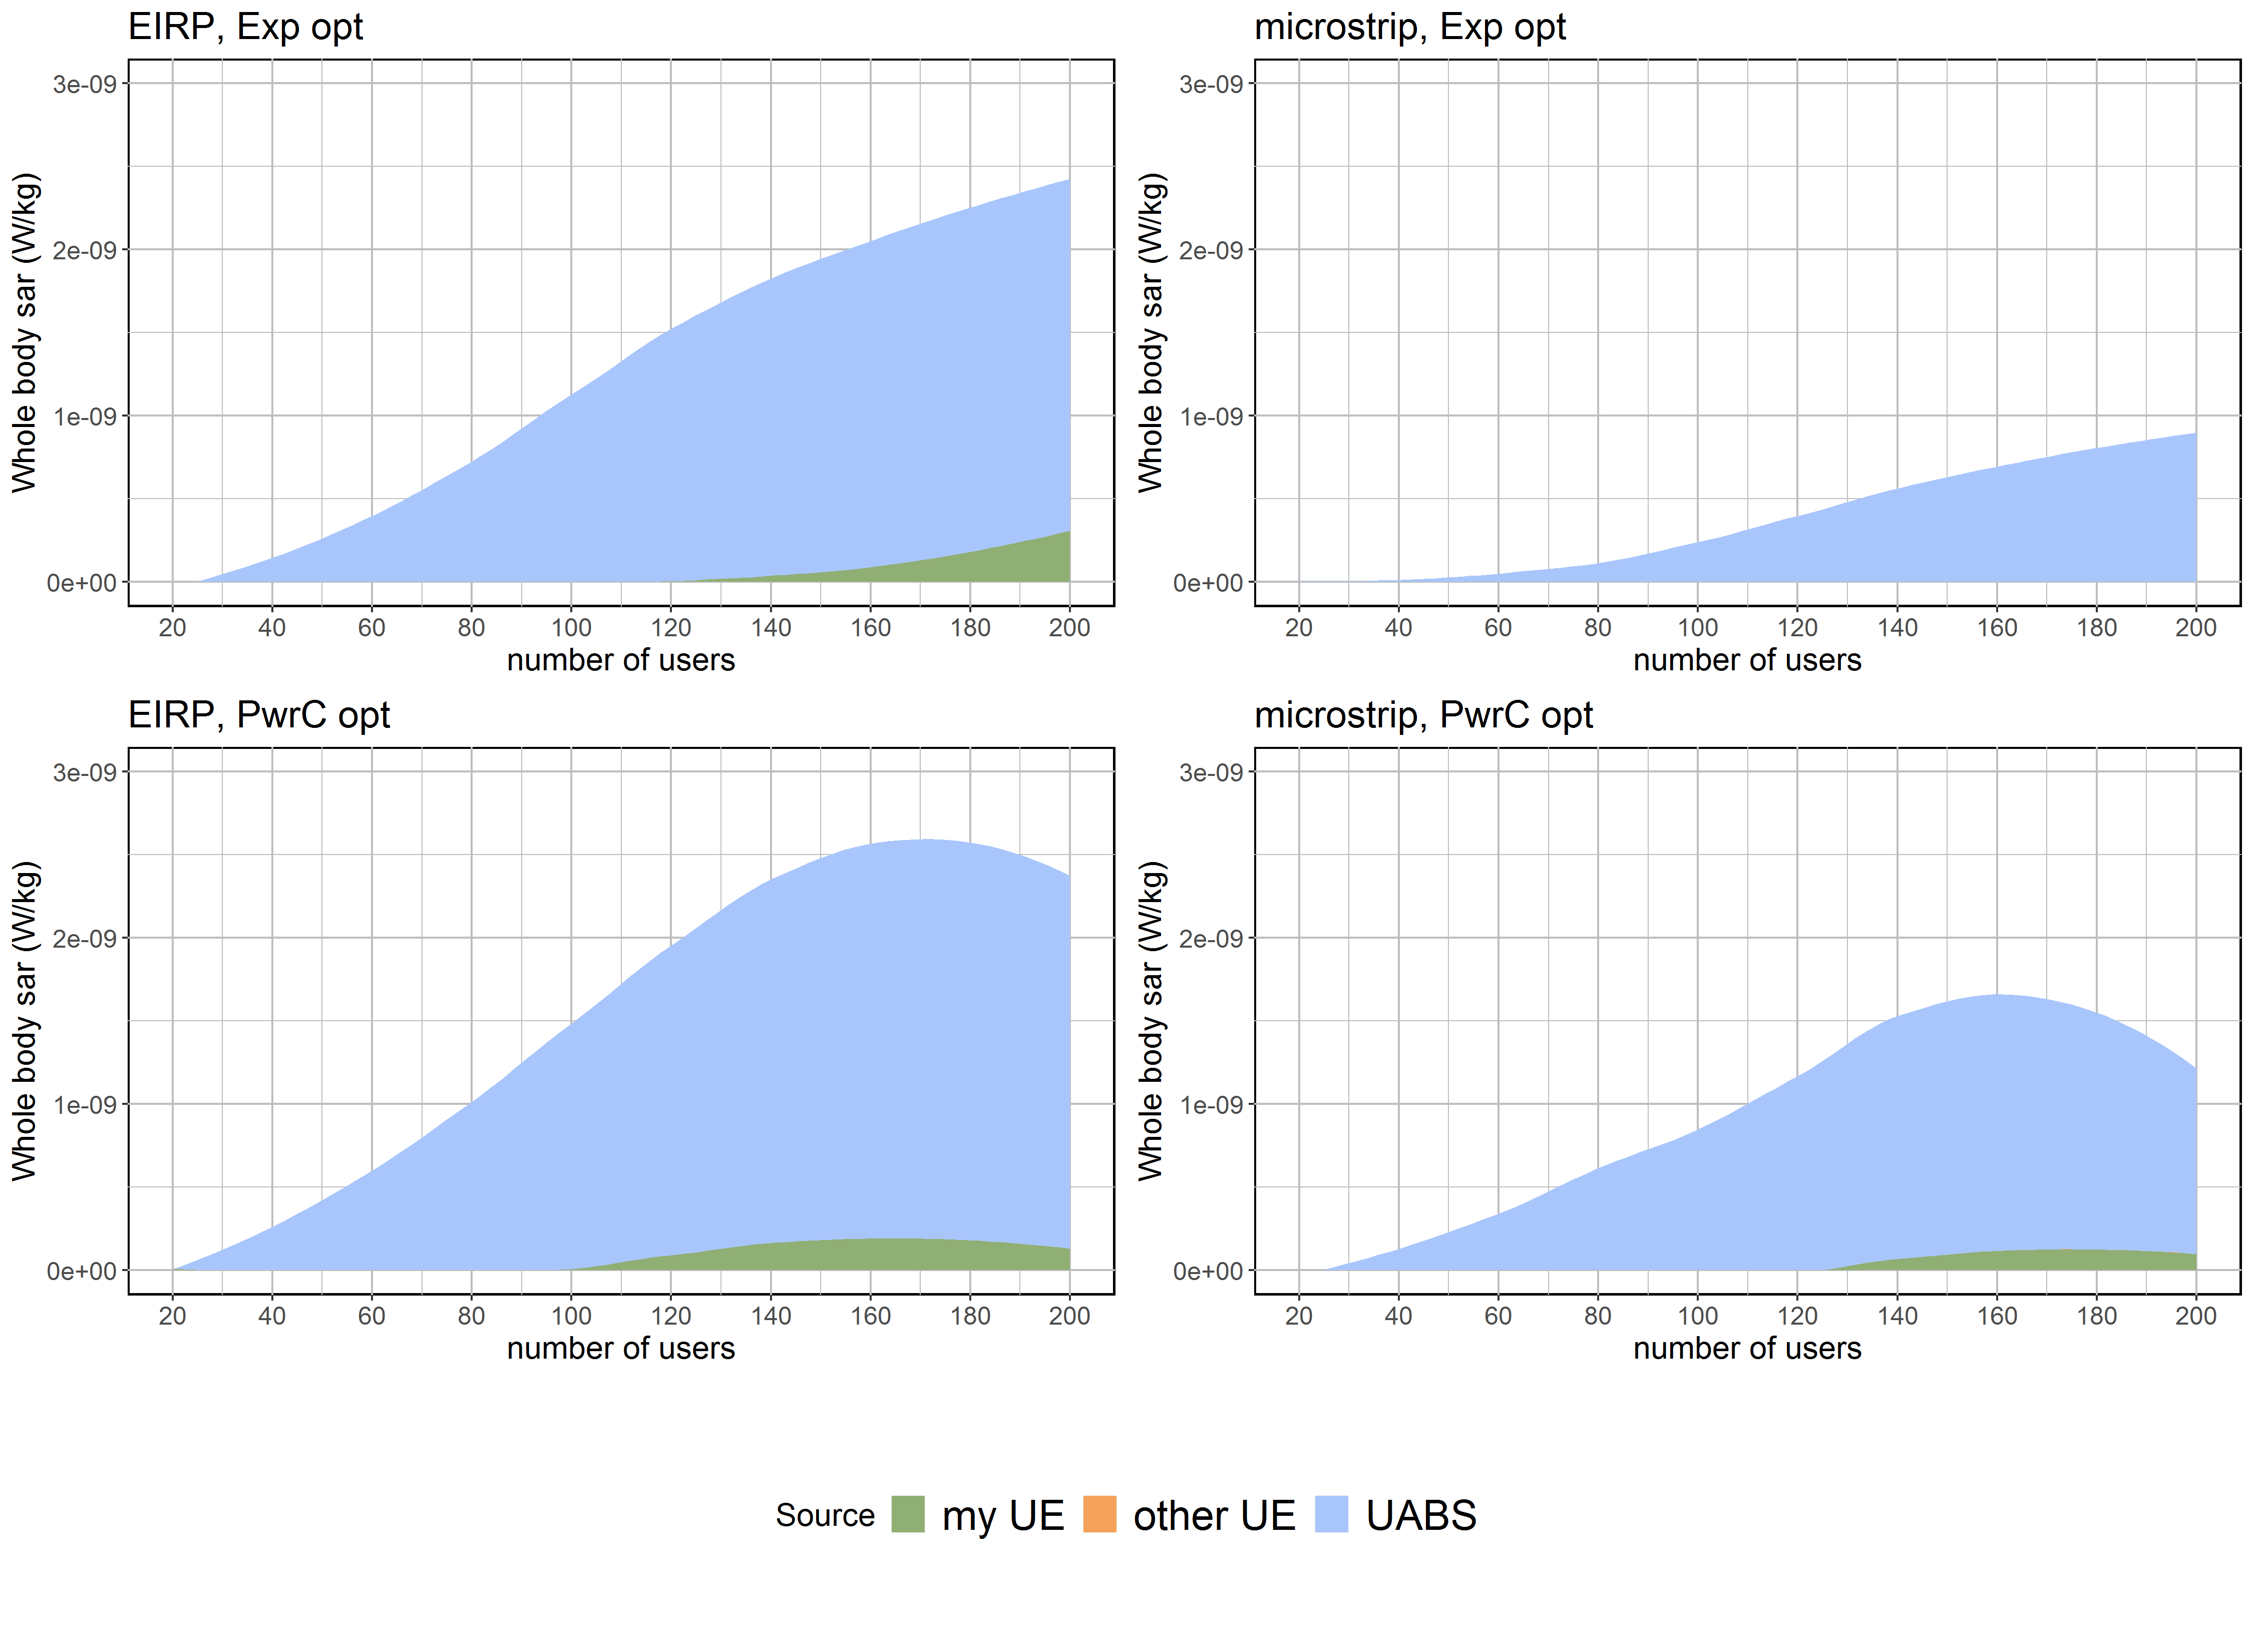
\includegraphics[width=\textwidth]{../results/s2/fhFourSources.png}
  \caption{Each figure corresponds with a certain configuration and shows how the \acs{SAR} from 
  different sources are influenced by an increasing flying height.}
  \label{fig:s2shfourSourcesMatrix}
\end{figure}

%%%%%%%%%%%%%%%%%%%%%%%%%%%%%%%%%%%%%%%%%%%%%%%%%%%%%%%%%%%%%%%%%%%%%%%%%%%%%%%%%%%%%%%%%%%%%%%%%%%%%%%%
\FloatBarrier
\subsection{Influence of the Number of Users}
\label{s2b}

The number of covered users increases linearly compared to the number of users present in the network as shown in figure 
\ref{fig:s2uvsnumcovusers}.b. It illustrates how an \gls{isotropicradiator} is able to reach more users 
compared to a microstrip patch antenna. Just like an power consumption optimized network 
is able to reach more users than an exposure optimized network.
For example, with 600 users, 5 to 7 additional 
people can be covered when replacing a microstrip patch antenna with an \gls{isotropicradiator}.
An changing an exposure optimized network with an power consumption optimized network will 
cover one or two additional users.
%This is because power consumption optimized networks will result in few high powered base stations while an 
%exposure optimized network results in a lot of low powered base stations. This behaviour will further be explained in section \ref{s3}

\begin{figure}[h!]
  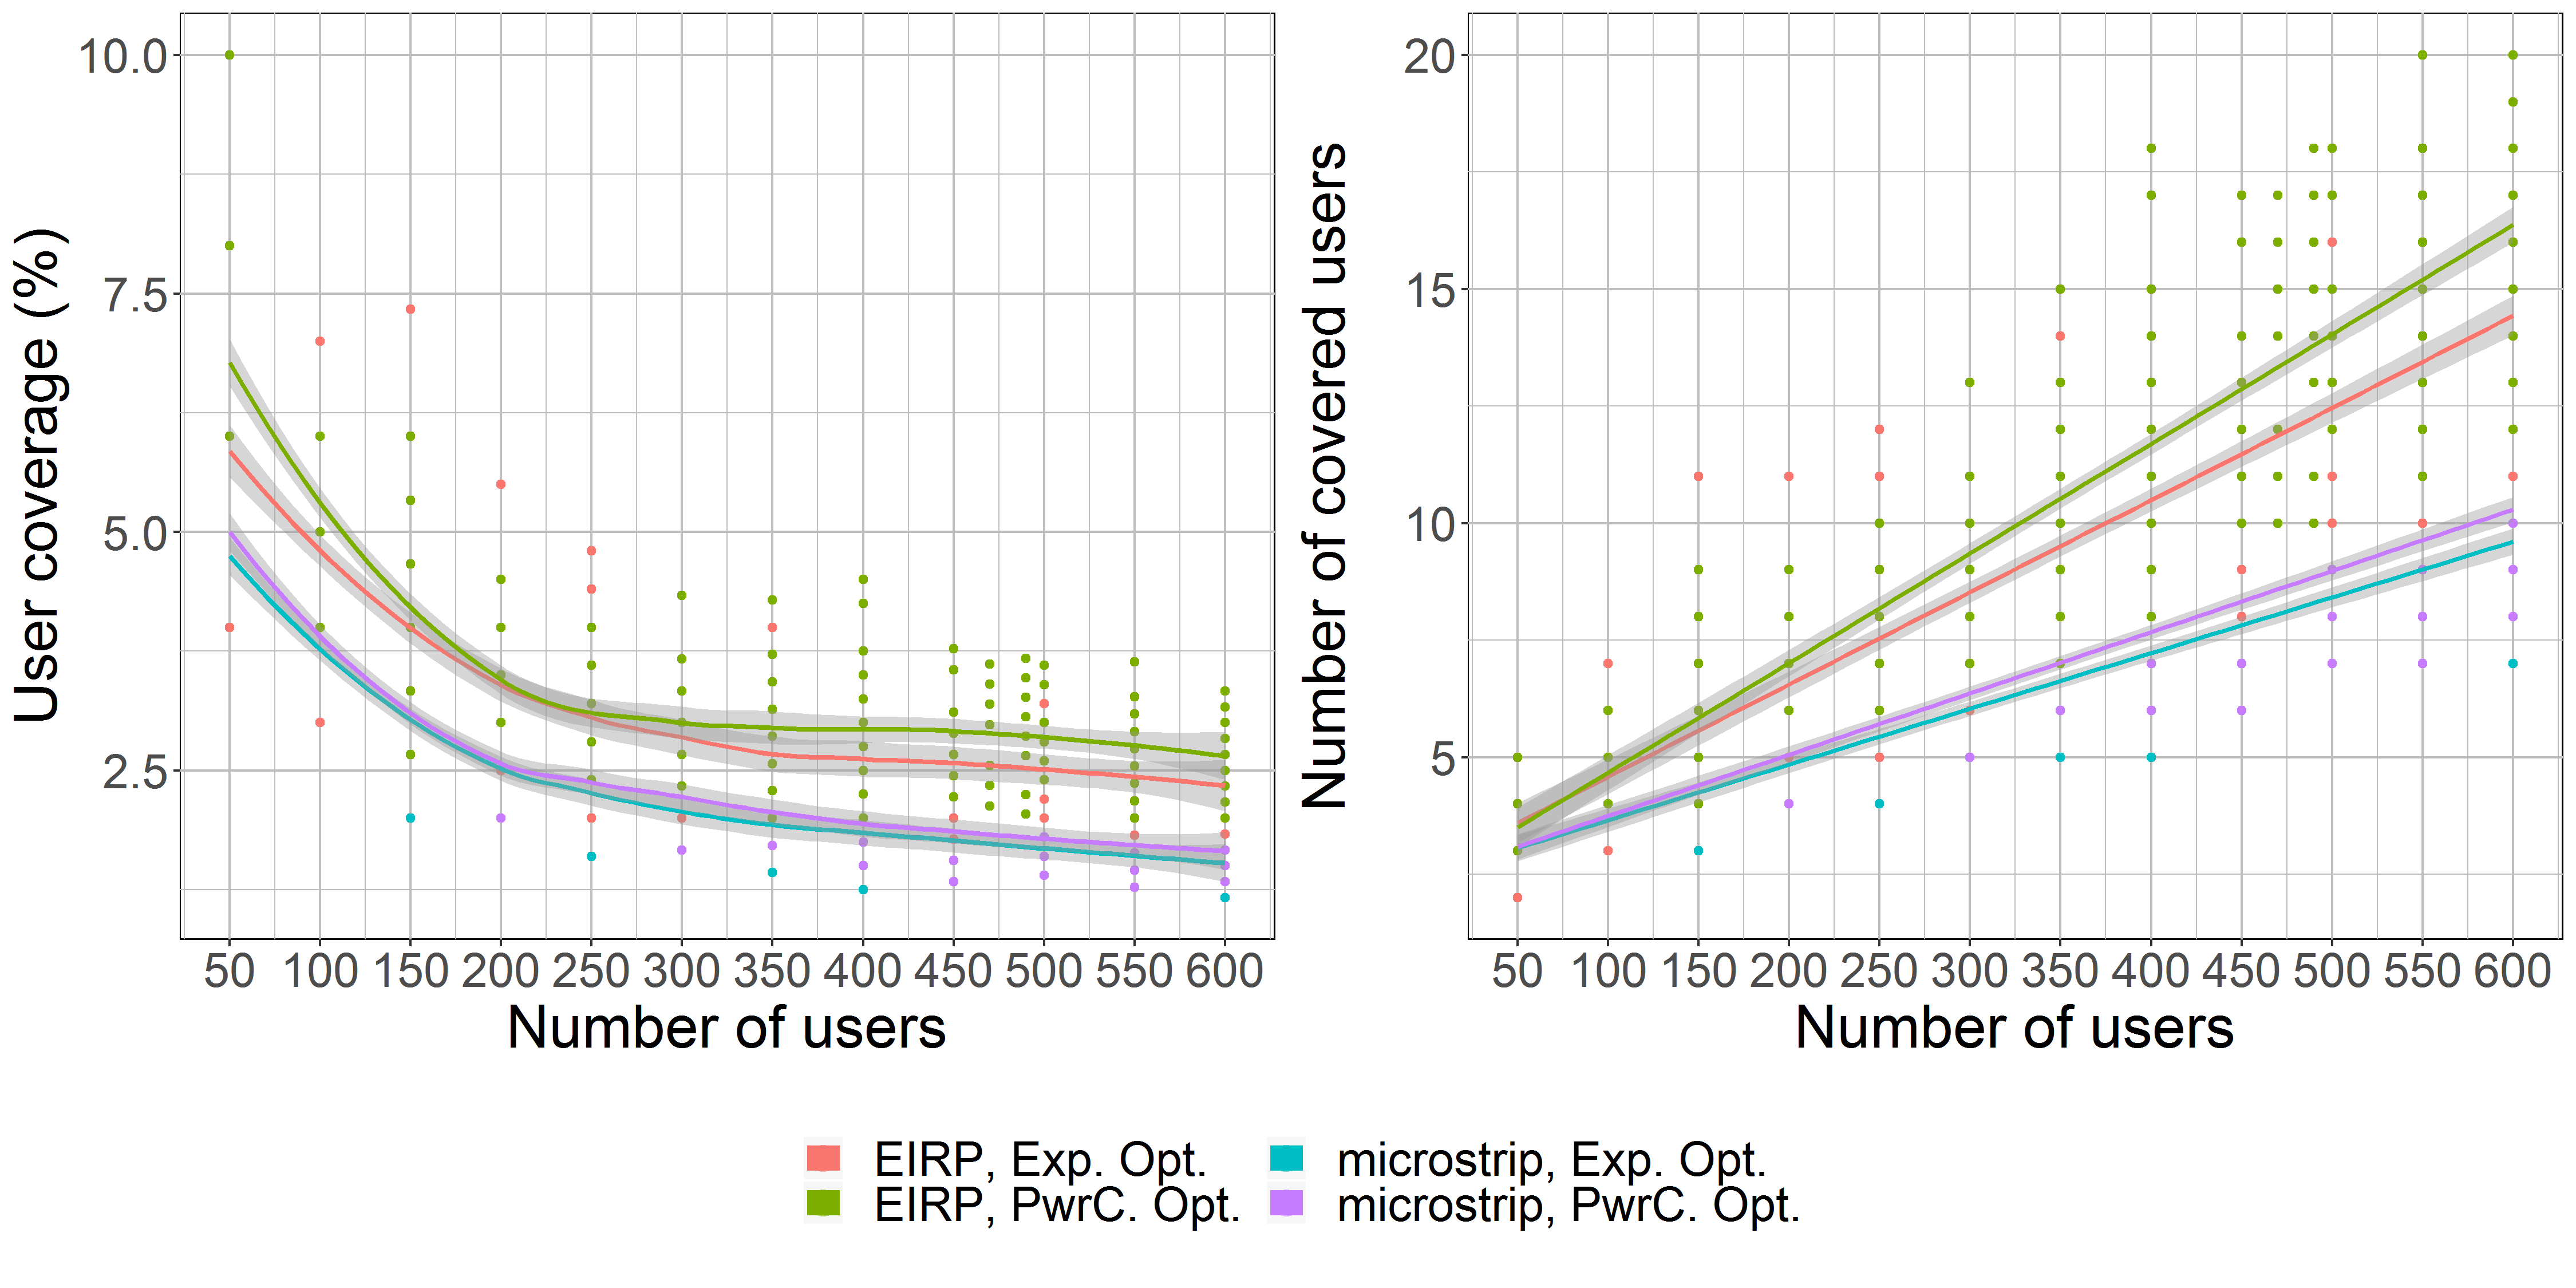
\includegraphics[width=\textwidth]{../results/s2/uvsnumdronesAndCov.png}
  \caption{The influence of increasing traffic on the user coverage.}
  \label{fig:s2uvsnumcovusers}
\end{figure}

The linear regression lines from figure \ref{fig:s2uvsnumcovusers} can be predicted with the equations in \ref{eq:numcovusers}.

\begin{equation}
\text{number of users =}
    \begin{cases}
      y = 0,0233x + 2,3553 & \text{if EIRP and PwrC Opt}\\
      y = 0,0197x + 2,6144  & \text{if EIRP and Exp Opt}\\
      y = 0,0131x + 2,4371  & \text{if microstrip and PwrC Opt}\\
      y = 0,0119x + 2,4652  & \text{if microstrip and Exp Opt}
    \end{cases} 
    \label{eq:numcovusers}      
\end{equation}

Figure \ref{fig:s2uvsnumcovusers}.a shows the percentage of covered users that follow out of \ref{fig:s2uvsnumcovusers}.b by taking the equations 
from \ref{eq:numcovusers} and dividing them by $x$.
This results in a decreasing logarithmic behaviour because the regression lines from  \ref{fig:s2uvsnumcovusers} have a slope of less than 0.5.
This means that the percentage of covered users for a small populated network is more compared to the percentage of users in large populations.
Figure \ref{fig:s2uvsnumcovusers} concludes that the increase in population causes a decrease in coverage since only 
one \gls{UABS} is available. While an \gls{EIRP} \gls{PwrC Opt} network with only 50 users knows  a 6.75\% coverage, a network with 600 users has no more than 2.75\% coverage.

\clearpage
Figure  \ref{fig:s2b_dlAndPc}.a  is influenced by  \ref{fig:s2uvsnumcovusers}.a. When less users are 
covered, the exposure of the average user will decrease as well.
For example, in an EIRP \gls{PwrC Opt} network, 50 users have a 6.75\% coverage which corresponds with a weighted average exposure of  18 $mV/m$
while 600 users with 2.75\% coverage only have 9 $mV/m$.
Further,  figure \ref{fig:s2b_dlAndPc}.b is directly influence by figure \ref{fig:s2uvsnumcovusers}.b. When the \gls{UABS} has to cover more users,
the probability that some of these users have a worse path loss is higher. The \gls{UABS} solves this problem by increasing the 
power consumption. Increasing the population from 50 to 600 will require between 0.05 and 0.1 $W$ more. 
For this scenario, no clear difference in power consumption exists between the four configurations.
\begin{figure}[h!]
  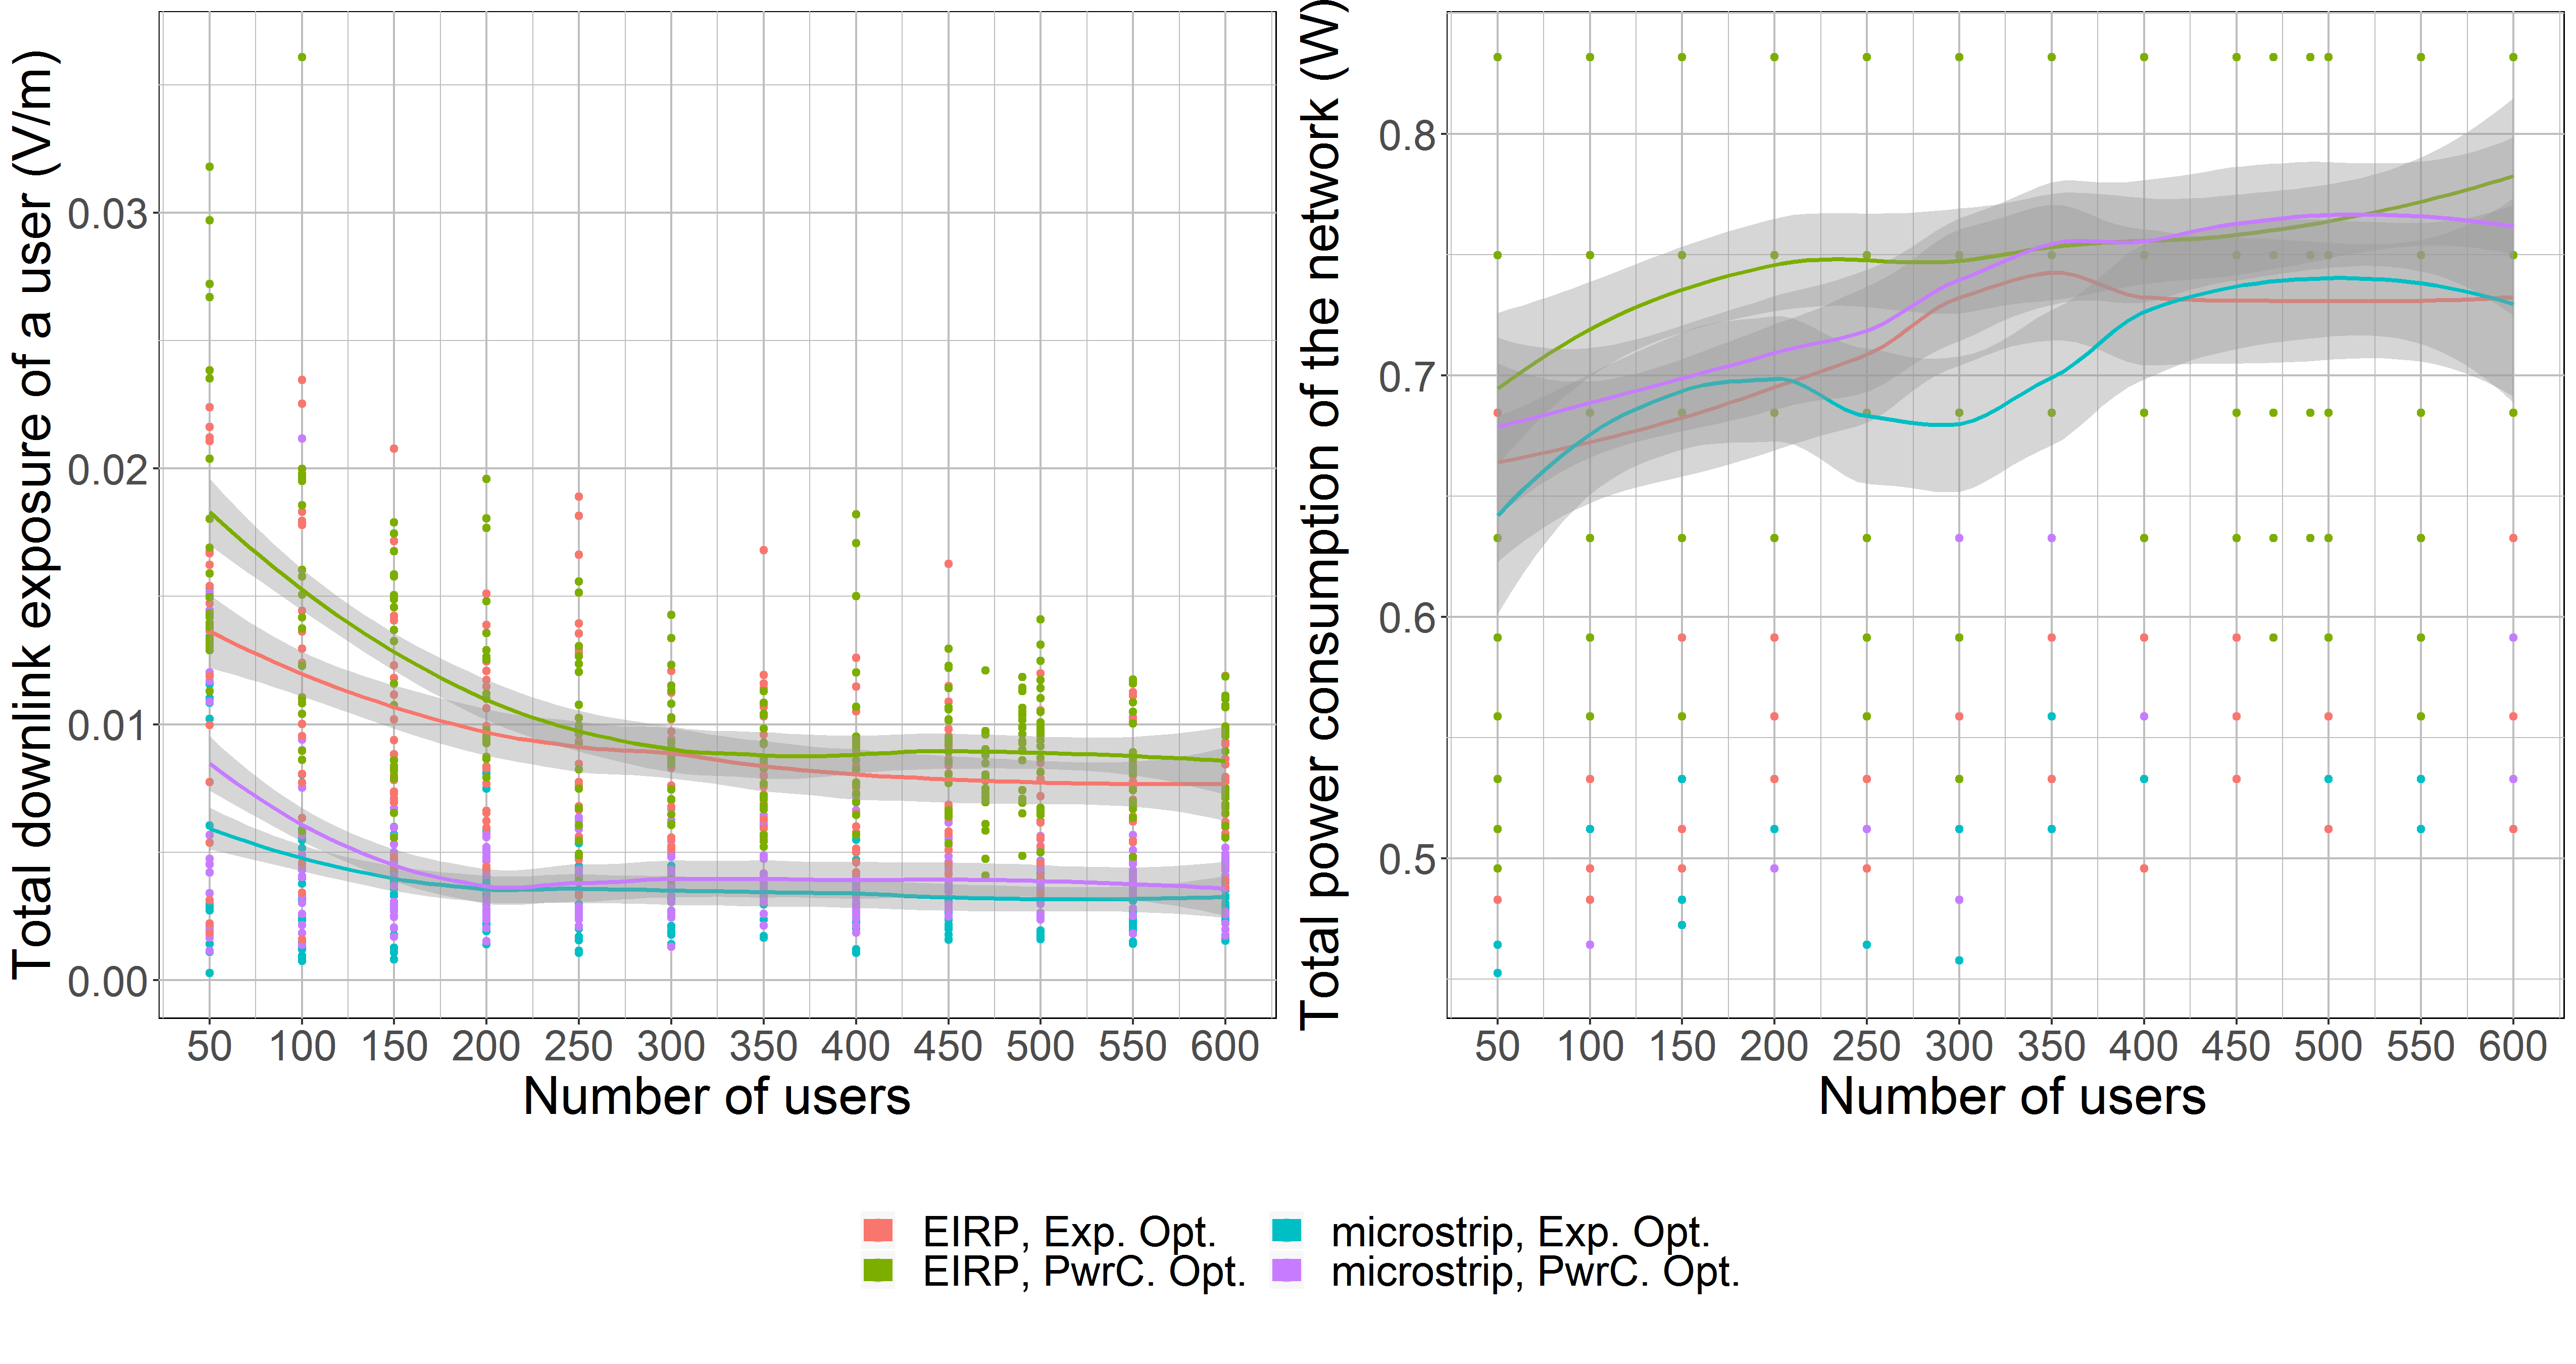
\includegraphics[width=\textwidth]{../results/s2/uvsdlAndPc.png}
  \caption{These two figures show how various sizes of population influence the downlink electromagnetic radiation of the average user (left) and 
  power consumption of the entire network (rights) for one \acs{UABS} available in the network.}
  \label{fig:s2b_dlAndPc}
\end{figure}

Figure \ref{fig:s2fourSourcesMatrix} investigates the assets of each source contributing to the total \gls{SAR}. All four 
configurations show that base stations are the main source of electromagnetic radiation which remains almost constant.
The \gls{isotropicradiator} varies around 1 $nW/kg$ for both optimizations and the microstrip antenna around 0.16 $nW/kg$.
Figure \ref{fig:s2uvsnumcovusers} already 
showed that a sparsely populated network results in a higher coverage percentage which on his turn results in a higher $SAR^{ownUE}$. 
The  $SAR^{ownUE}$ for 50 users is for an \gls{isotropicradiator} on average 1.7 $nW/kg$ for both optimizations and the microstrip antenna around 0.4 $nW/kg$.
The chart also proves once again that the far-field radiation from \gls{UE} can be neglected. The \gls{SAR} from 
neighbouring devices is not zero as it looks like in figure \ref{fig:s2fourSourcesMatrix} but is just really low compared to the much higher
\gls{SAR}-values from other sources.
\begin{figure}[h!]
\centering
  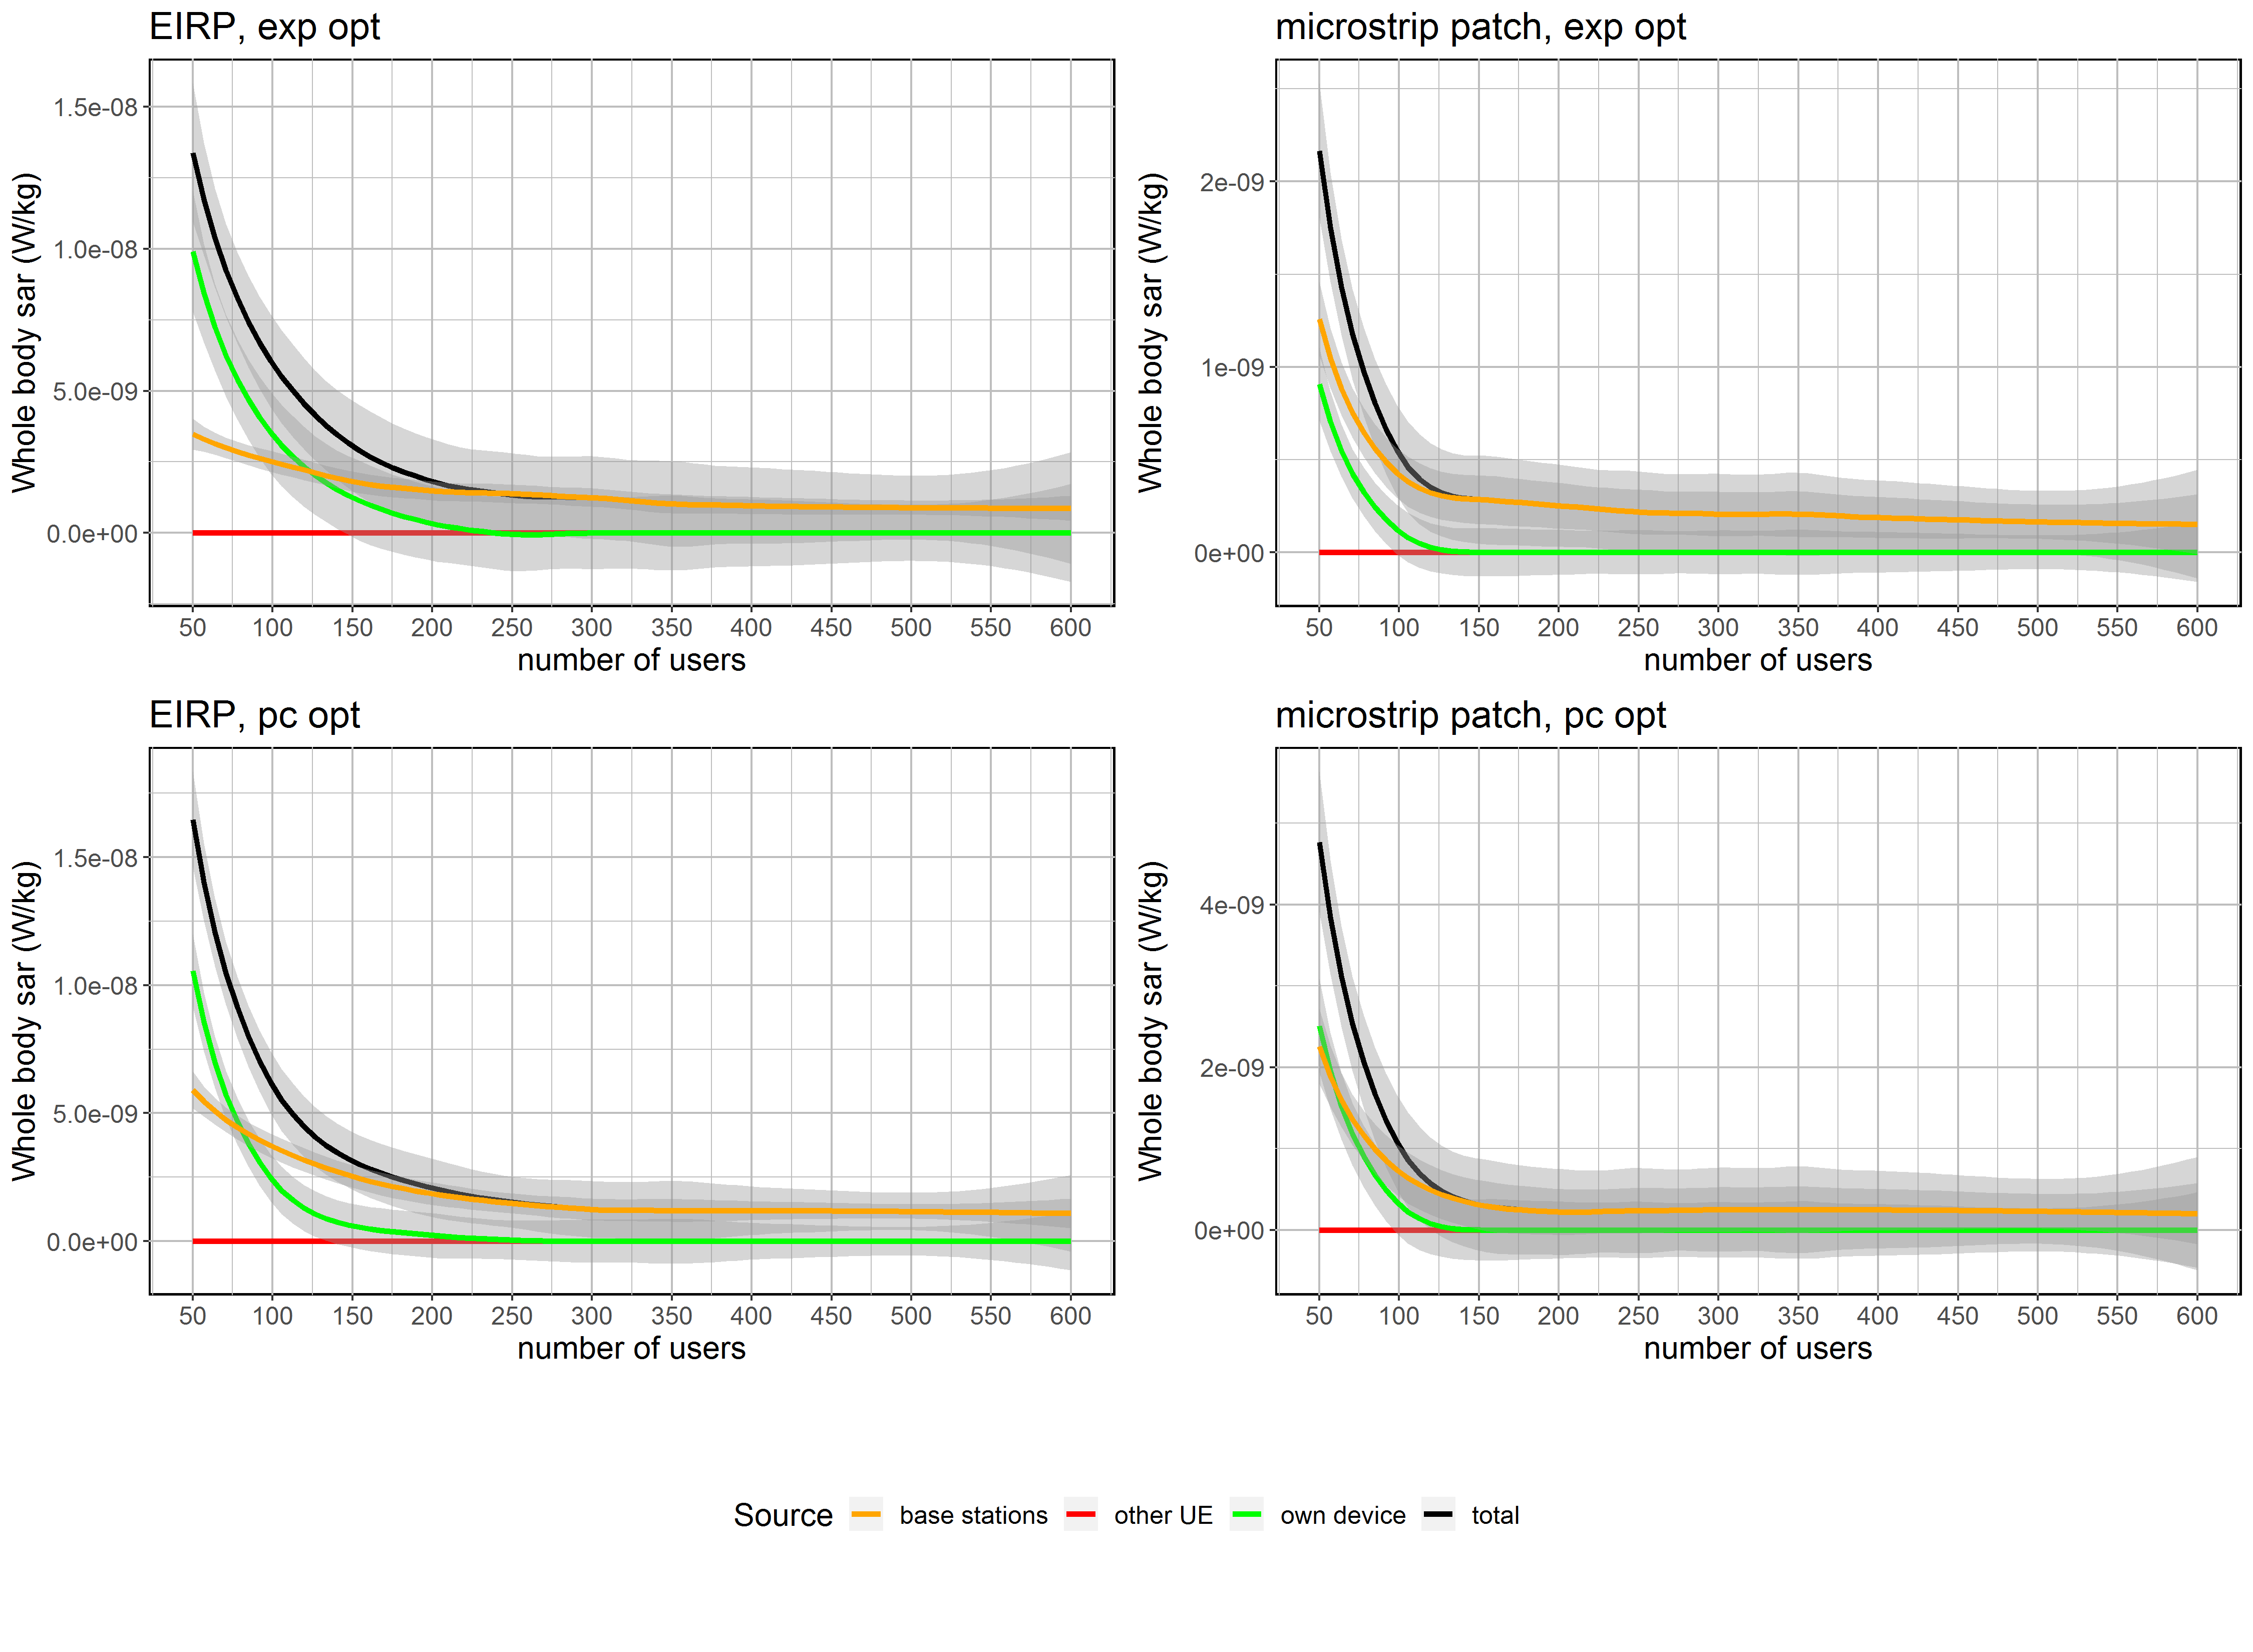
\includegraphics[width=\textwidth]{../results/s2/uFourSources.png}
  \caption{This figure shows how different sources are influenced by an increasing number of users. }
  \label{fig:s2fourSourcesMatrix}
\end{figure}

While the population grows, more and more users become uncovered causing the average SAR to drop. 
However, this does not conclude that  by increasing the population, the SAR of a user who is directly beneath a \gls{UABS} would be less.
To investigate this, a user is positioned in the middle of the city centre of Ghent and a \gls{UAV} is positioned above him. Initially, only 
49 people are active around him. The \gls{SAR} of our central user is monitored while the population around him is growing.
Figure \ref{fig:connectionMap} shows with the black lines which users are connected. Figure \ref{fig:connectionMap}.a is for only 50 users and 
shows that only one user is connected besides our central user. Figure \ref{fig:connectionMap}.b considers 600 users and shows much more connected users.
\begin{figure}[h]
\subfloat[50 users]{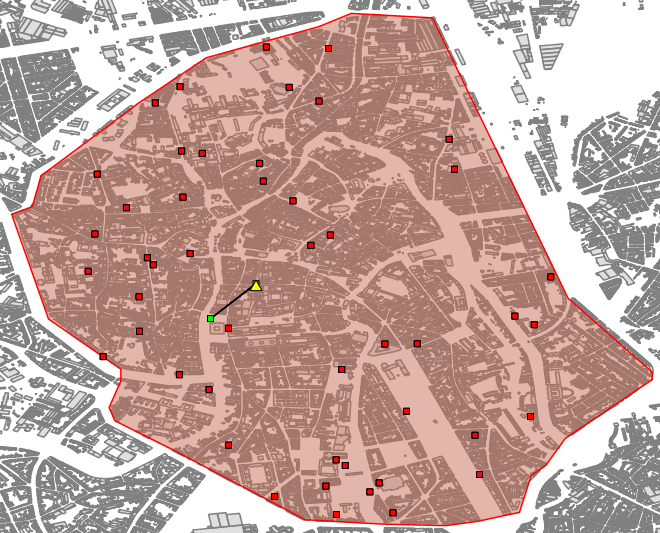
\includegraphics[width=0.49\textwidth]{../images/connectionsMap50Users.png}}
\hfill
\subfloat[600 users]{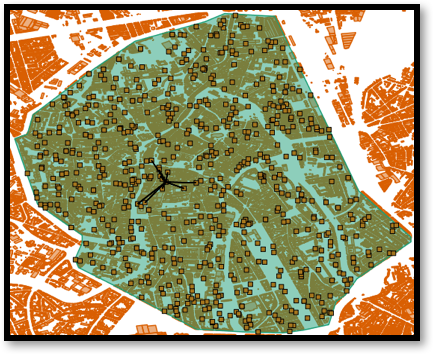
\includegraphics[width=0.49\textwidth]{../images/connectionsMap600Users.png}}
\caption{Overview of which users are connected to the \acs{UABS}.}
  \label{fig:connectionMap}
\end{figure}
Scenario I already showed that the \gls{SAR} from the user's own device is only influenced by the flying height. 
The flying height for this experiment is fixed and the \gls{UL} \gls{SAR} from his device should therefore also be a constant. 
A hypothesis that is confirmed by figure \ref{fig:uvsulsarcentralUsers}.a where $SAR^{myUE}$ is equal to 0.15 $\mu W/kg$.
The \gls{SAR} from the \gls{UABS} experiences a slight increase of 0.005 $\mu W/kg$. When the population grows, more users become available 
and some will spawn near the central user. The \gls{UABS} will likely decide to cover these users as well as visible in figure \ref{fig:connectionMap}.
These users might have a slightly 
worse path loss because of obstructing buildings or somewhat bigger distance. The \gls{UABS} reacts to this by increasing 
his power consumption causing an increase in the \gls{DL} \gls{SAR} for the central user.
The far-field radiation from \gls{UE} is very low as mentioned before and therefore added separately in figure \ref{fig:uvsulsarcentralUsers}.b.
It shows that the \gls{SAR}  from other \gls{UE} increases from zero to $0.15\ pW/kg$. This is normal 
behaviour considering that around the central user more and more people become available of which some will be connected to the \gls{UABS}
and therefore also emitting radiation.
\begin{figure}[hb]
\centering
  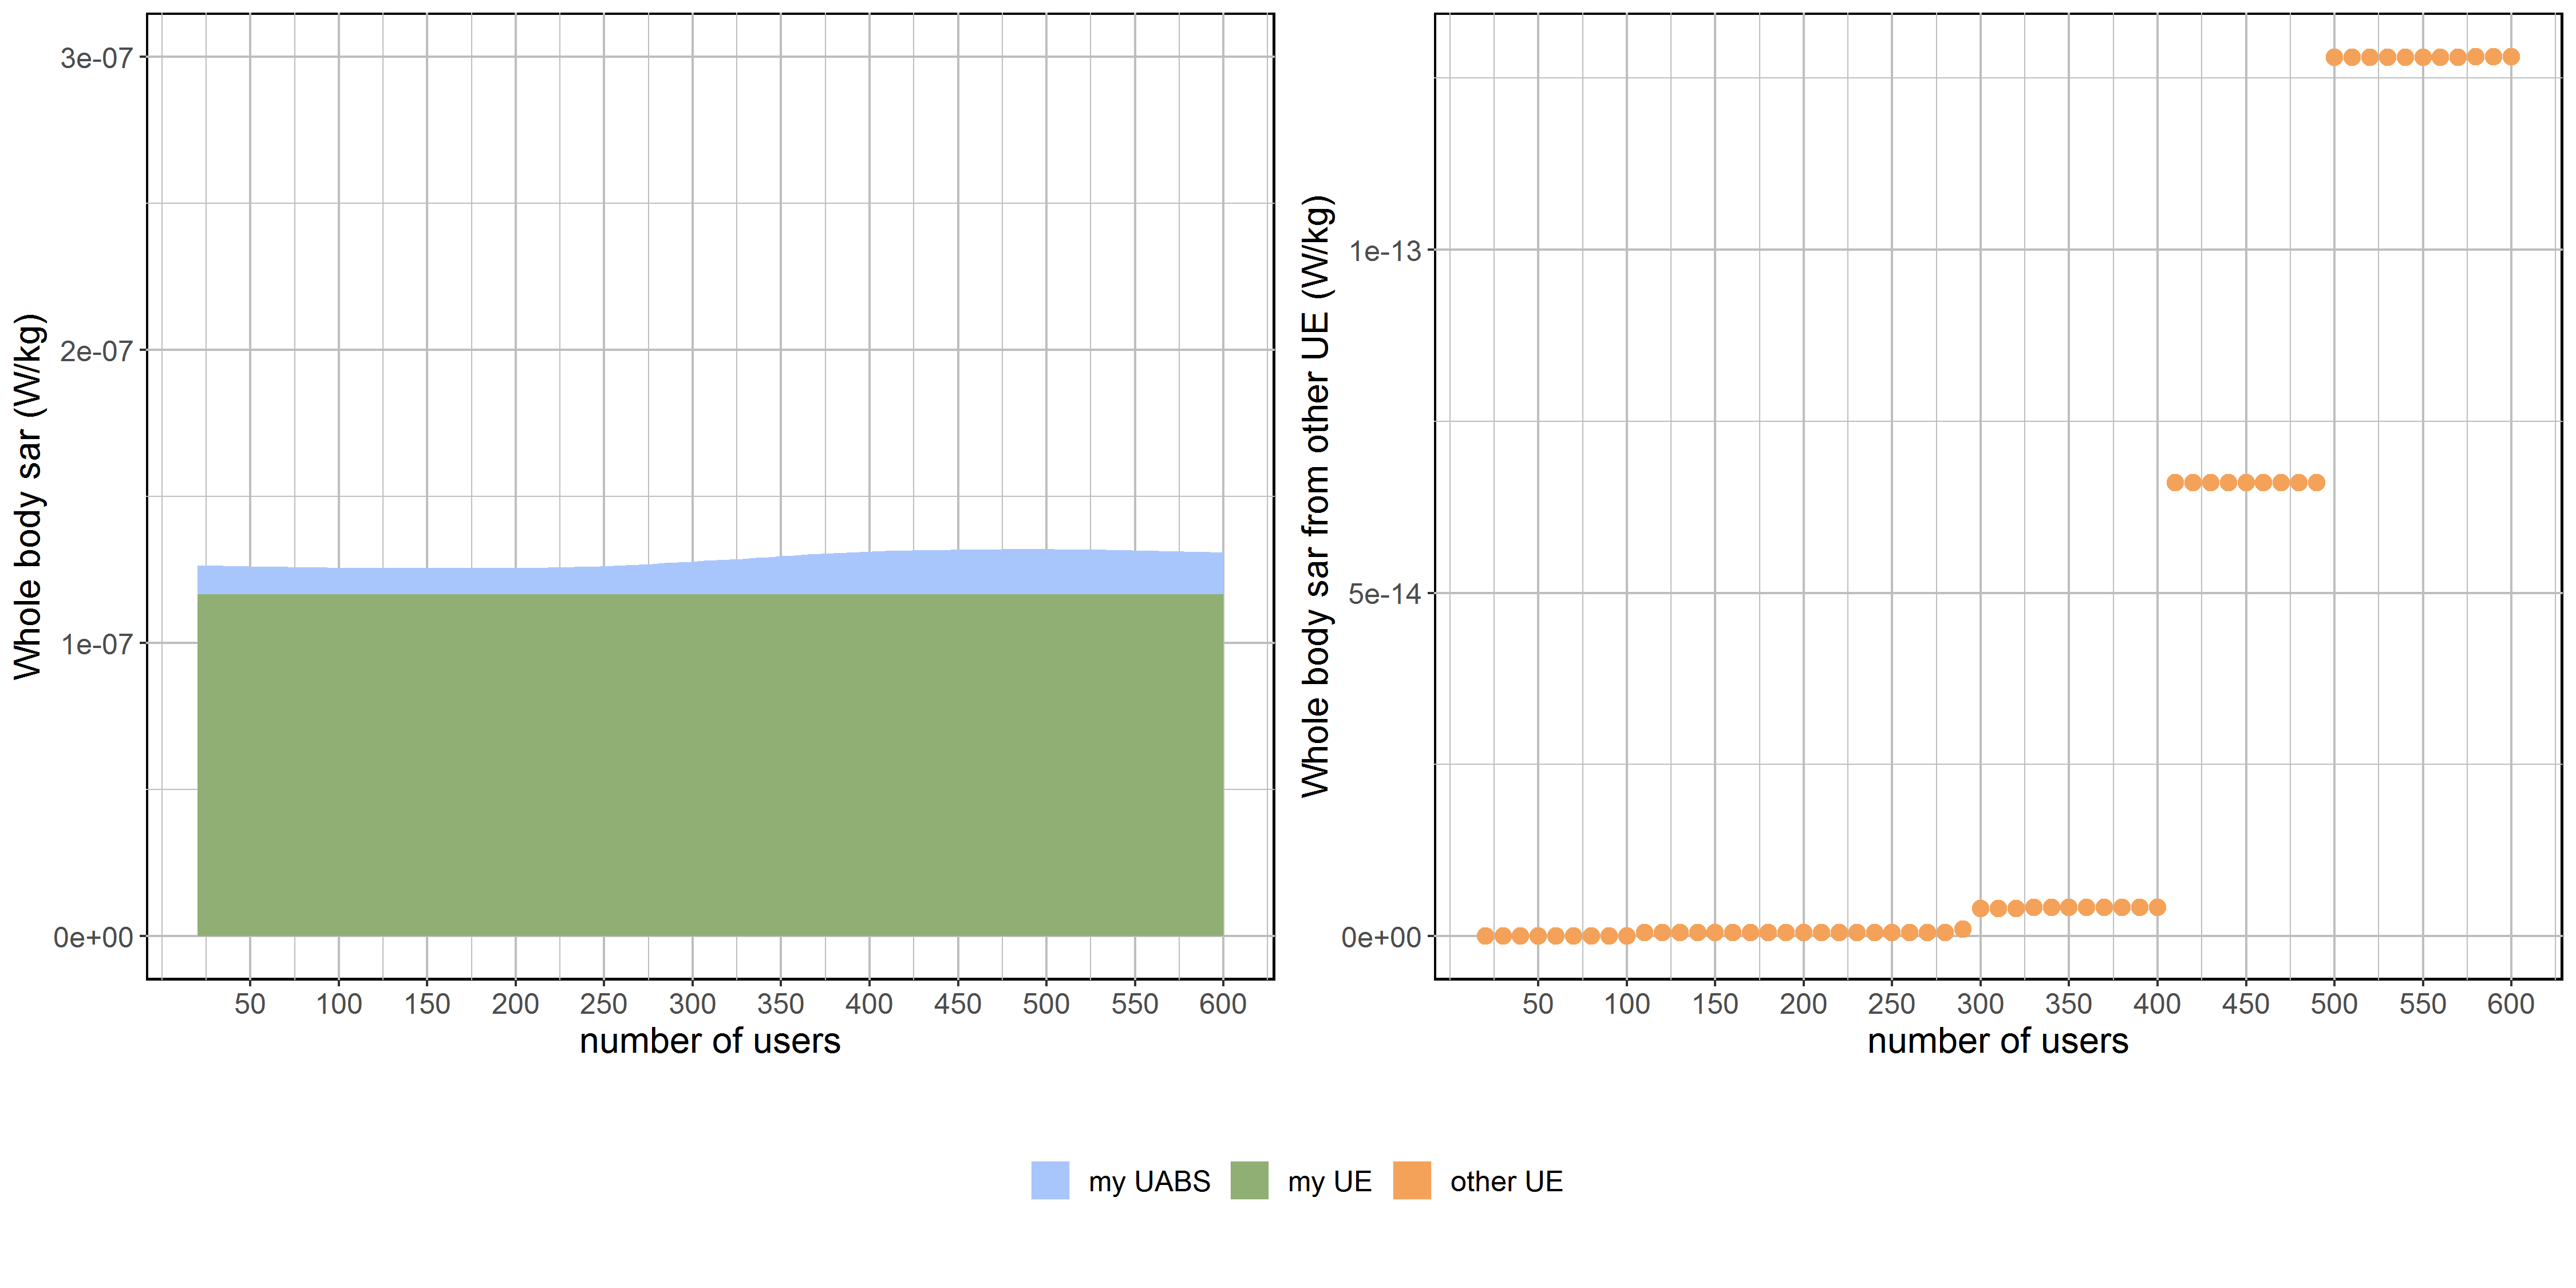
\includegraphics[width=0.9\textwidth]{../results/s2/uvsulsarcentralUser.png}
  \caption{SAR-values for the user who is directly beneath the only \acs{UABS} available.}
  \label{fig:uvsulsarcentralUsers}
\end{figure}

%%%%%%%%%%%%%%%%%%%%%%%%%%%%%%%%%%%%%%%%%%%%%%%%%%%%%%%%%%%%%%%%%%%%%%%%%%%%%%%%%%%%%%%%%%%%%%%%%%%%%%%%%%%%%s
\FloatBarrier
\section{Scenario III: Unlimited \gls{UAV}s}
\label{s3}

This scenario, just like the previous one, has much more users in the network 
and investigates the same cases which include the variable flying height and the variable number of  users.
The only difference is that the restriction of only one \gls{UABS} is dropped.
An example is presented in figure \ref{fig:s3:distribution}.
\begin{figure}[!htb]
  \subfloat[microstrip, \gls{Exp Opt} ]{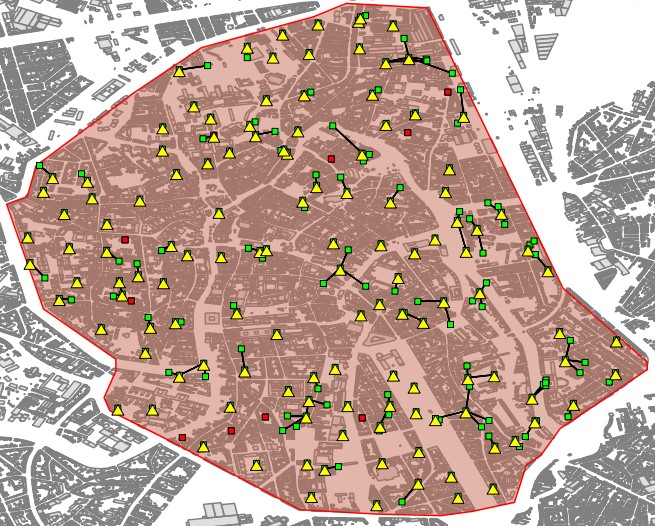
\includegraphics[width=0.49\textwidth]{../images/ghentDistribution_expmicro_drones.jpg}}
  \hfill
  \subfloat[EIRP, \gls{PwrC Opt}]{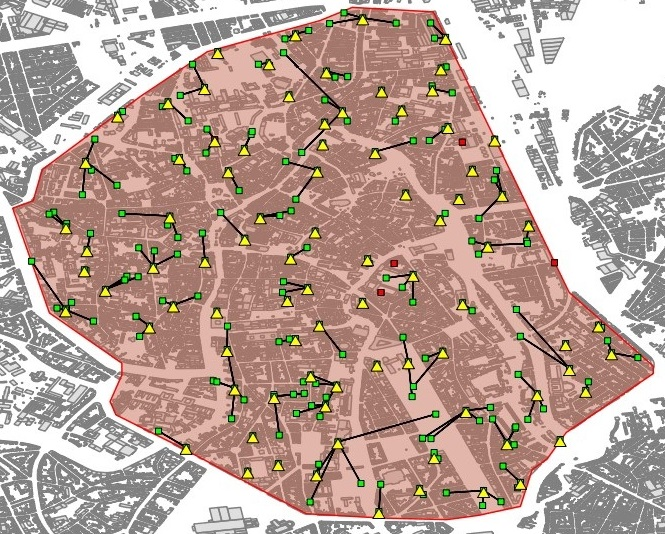
\includegraphics[width=0.49\textwidth]{../images/ghentDistribution_pcEIRP_drones.jpg}}
  \caption{Example of two networks with users distributed over the area. Yellow triangles represent \acs{UABS}s and are connected 
  with black lines to users in green. Uncovered users are coloured in red.}
  \label{fig:s3:distribution}
\end{figure}

\subsection{Influence of the Flying Altitude}
\label{S3A}
The first evaluated parameter of this scenario is the flying height
with a fixed number of 224 users.
Scenario II already explained that when only one \gls{UAV} is available, a power consumption optimized network will not result in a low 
powered network. In this scenario, there is no limitation on the number of \gls{UAV}s and the network remains thus unaltered after the decision 
algorithm is done. Figure \ref{fig:s3a_dlAndPc} proves that the different optimization strategies work as intended.
Power consumption optimized networks have indeed a lower power consumption but therefore result in higher electromagnetic radiation.
On the other hand, an exposure optimized network will reduce the electromagnetic exposure by using more \gls{UAV}s and thence also increases the network's power consumption.
A behaviour that was also concluded in \cite{J1}.
For example, when comparing both optimization strategies for the same \gls{isotropicradiator} and the same default flying height, we see that
the power consumption optimized network requires 51 $W$ and therefore exposes its users
to $15\ mV/m$. When optimizing towards electromagnetic radiation, the exposure drops to $11.5\ mV/m$ but at a cost of a higher power consumption
of $54\ W$.
\begin{figure}[h!]
\centering
  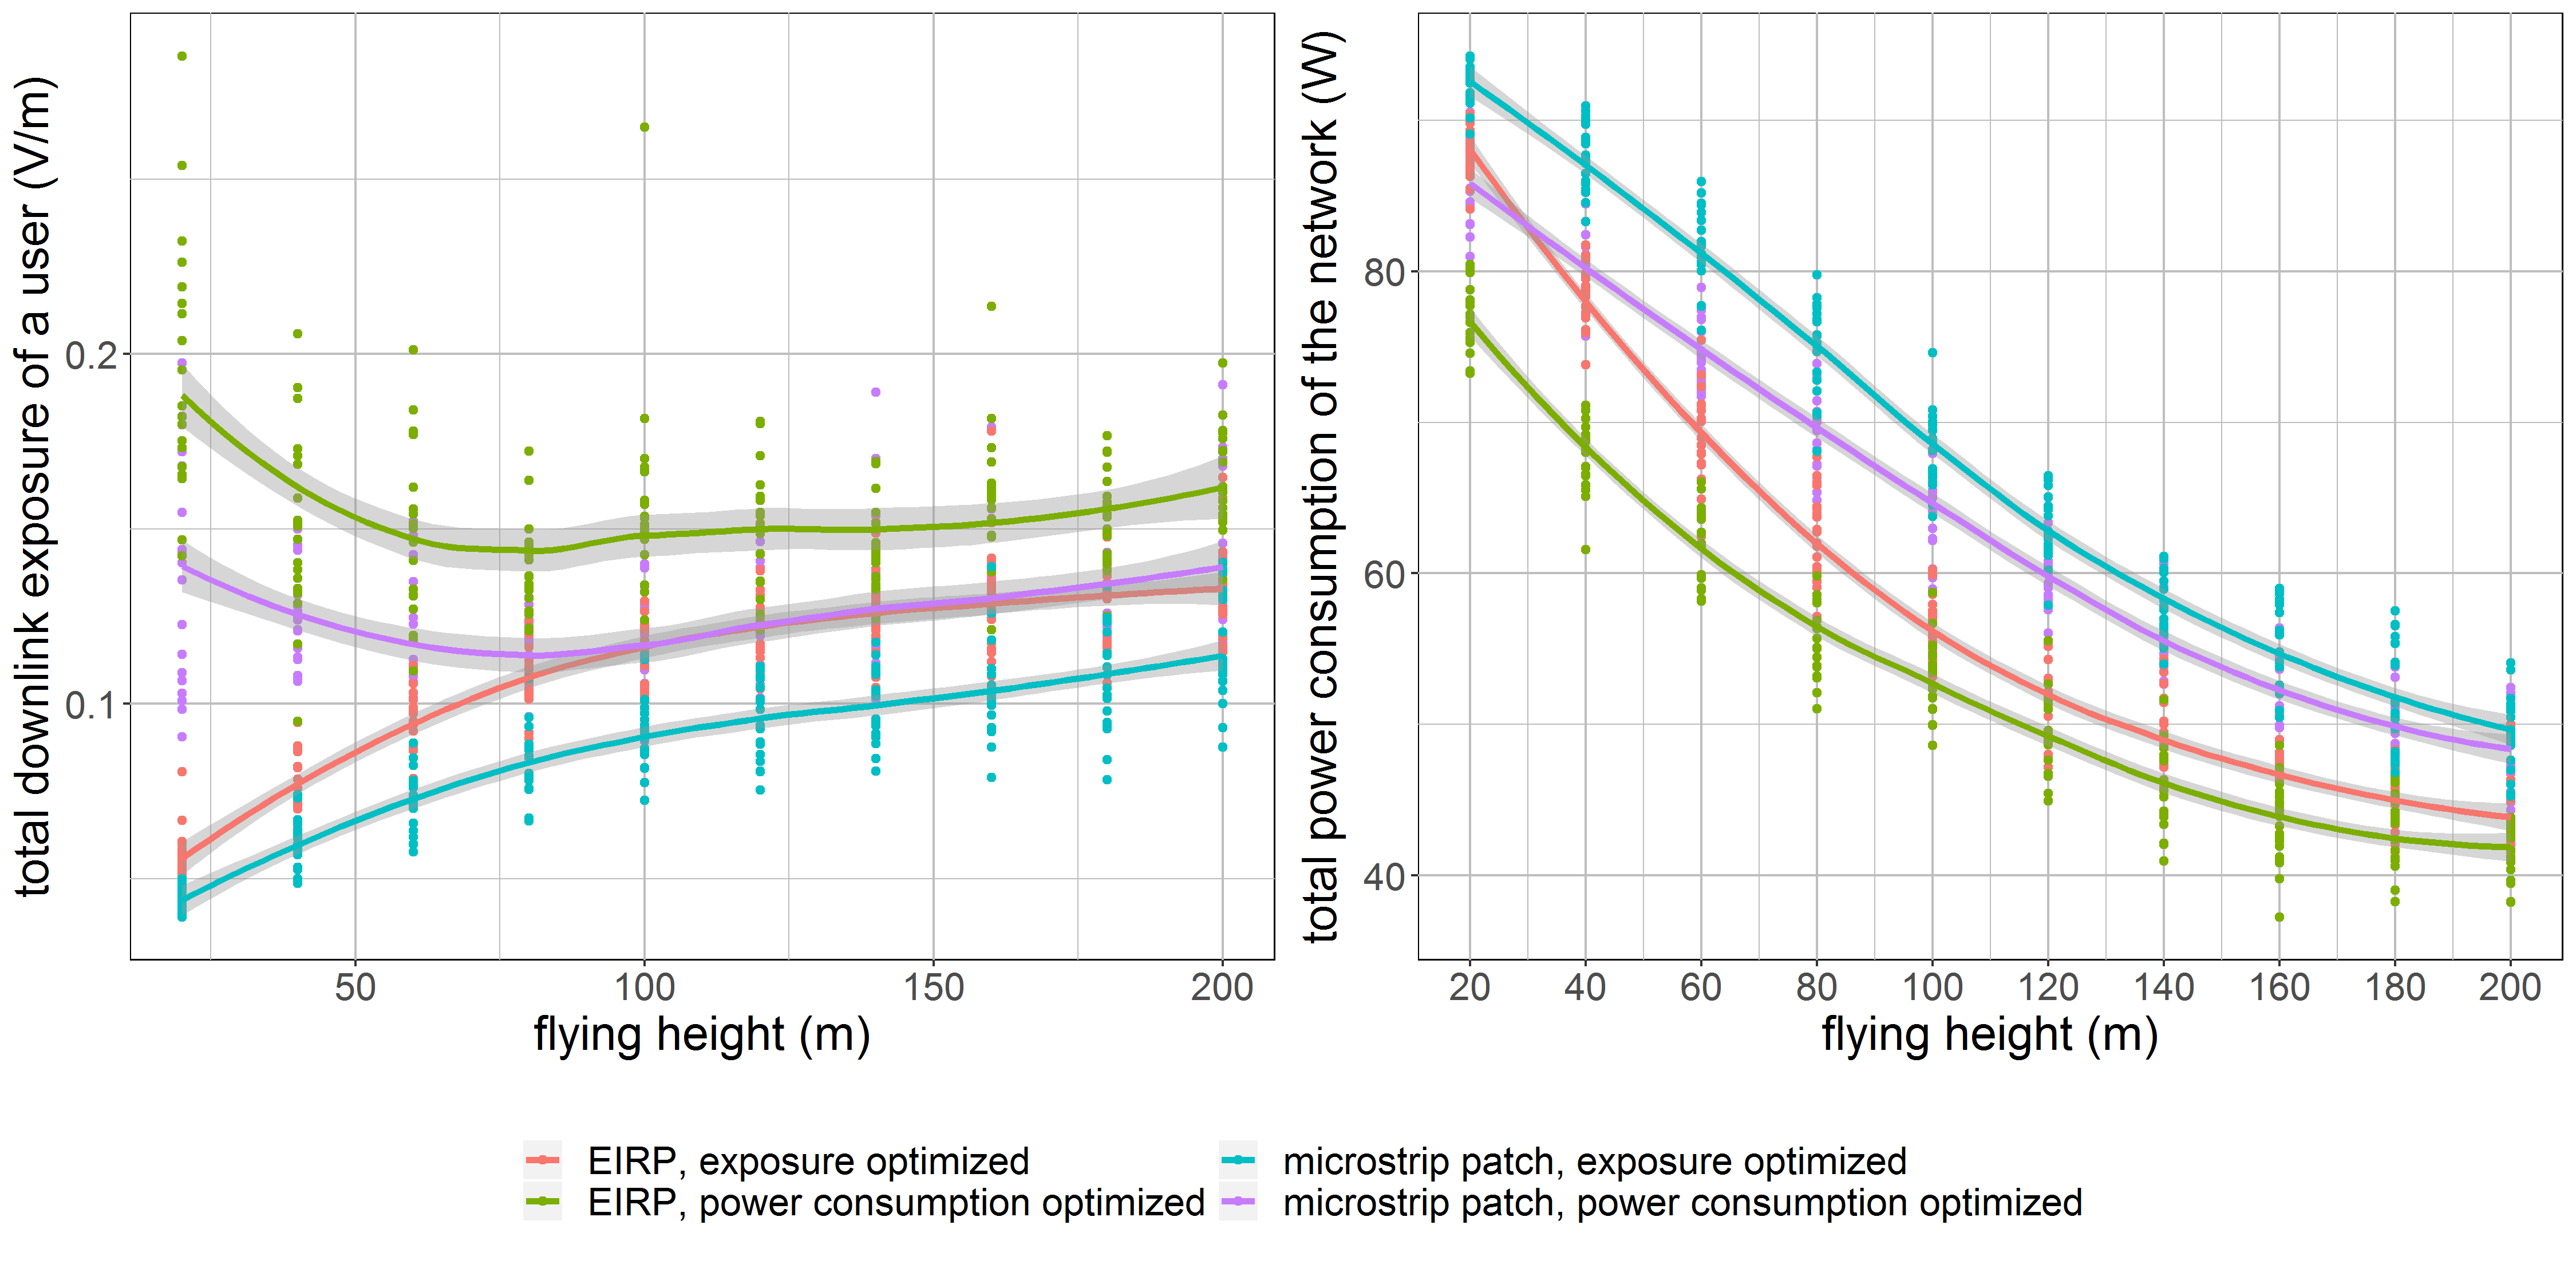
\includegraphics[width=\textwidth]{../results/s3/fhvsdlAndPc.png}
  \caption{
    These two figures show how the flying height influences the downlink electromagnetic radiation of the average user (left) and 
  power consumption of the entire network (right) for an unlimited number of drones.
  }
     \label{fig:s3a_dlAndPc}
\end{figure}

Further, figure  \ref{fig:s3a_dlAndPc}.a also shows that the exposure in an exposure optimized network increases logarithmically while in a power consumption optimized network the exposure has a concave relationship with the flying height, and has its lowest point at around 70 metres.
%Figure \ref{fig:s3a_dlAndPc} shows that the decrease in electromagnetic exposure comes at a cost of increased power consumption.
%This increase is caused by the much higher amount of required drones as visible in figure \ref{fig:s3a_numDronesAndCov}.
%The fitness function in equation \ref{eq:fitnessfunction} penalise large path losses because they increase electromagnetic radiation.
%The tool solves this problem by assigning a \gls{UABS} more nearby. Therefore, we notice in 
%figure \ref{fig:s3a_numDronesAndCov}.b that at a default flying altitude, exposure optimized networks require on average 15 drones more 
%than the power consumption optimized network for both antenna types.
Figure \ref{fig:s3a_numDronesAndCov}.a shows that the optimal coverage is achieved at a low flying height of 
40 metres with around 99\% coverage. 
However, there is a downside to this. 
Figure \ref{fig:s3a_numDronesAndCov}.b 
 shows that the number of required \gls{UAV}s increases when the flying altitude becomes lower;
a behaviour which was also determined in \cite{J2}.
For example, an microstrip \gls{Exp Opt} network and an \gls{EIRP} \gls{PwrC Opt} network require respectively 84 and 64
\gls{UABS}s at a flying altitude of $200\ m$ which increases respectively to 211 and 162 \gls{UABS}s at a much lower flying altitude of $20\ m$.
\begin{figure}[h!]
\centering
  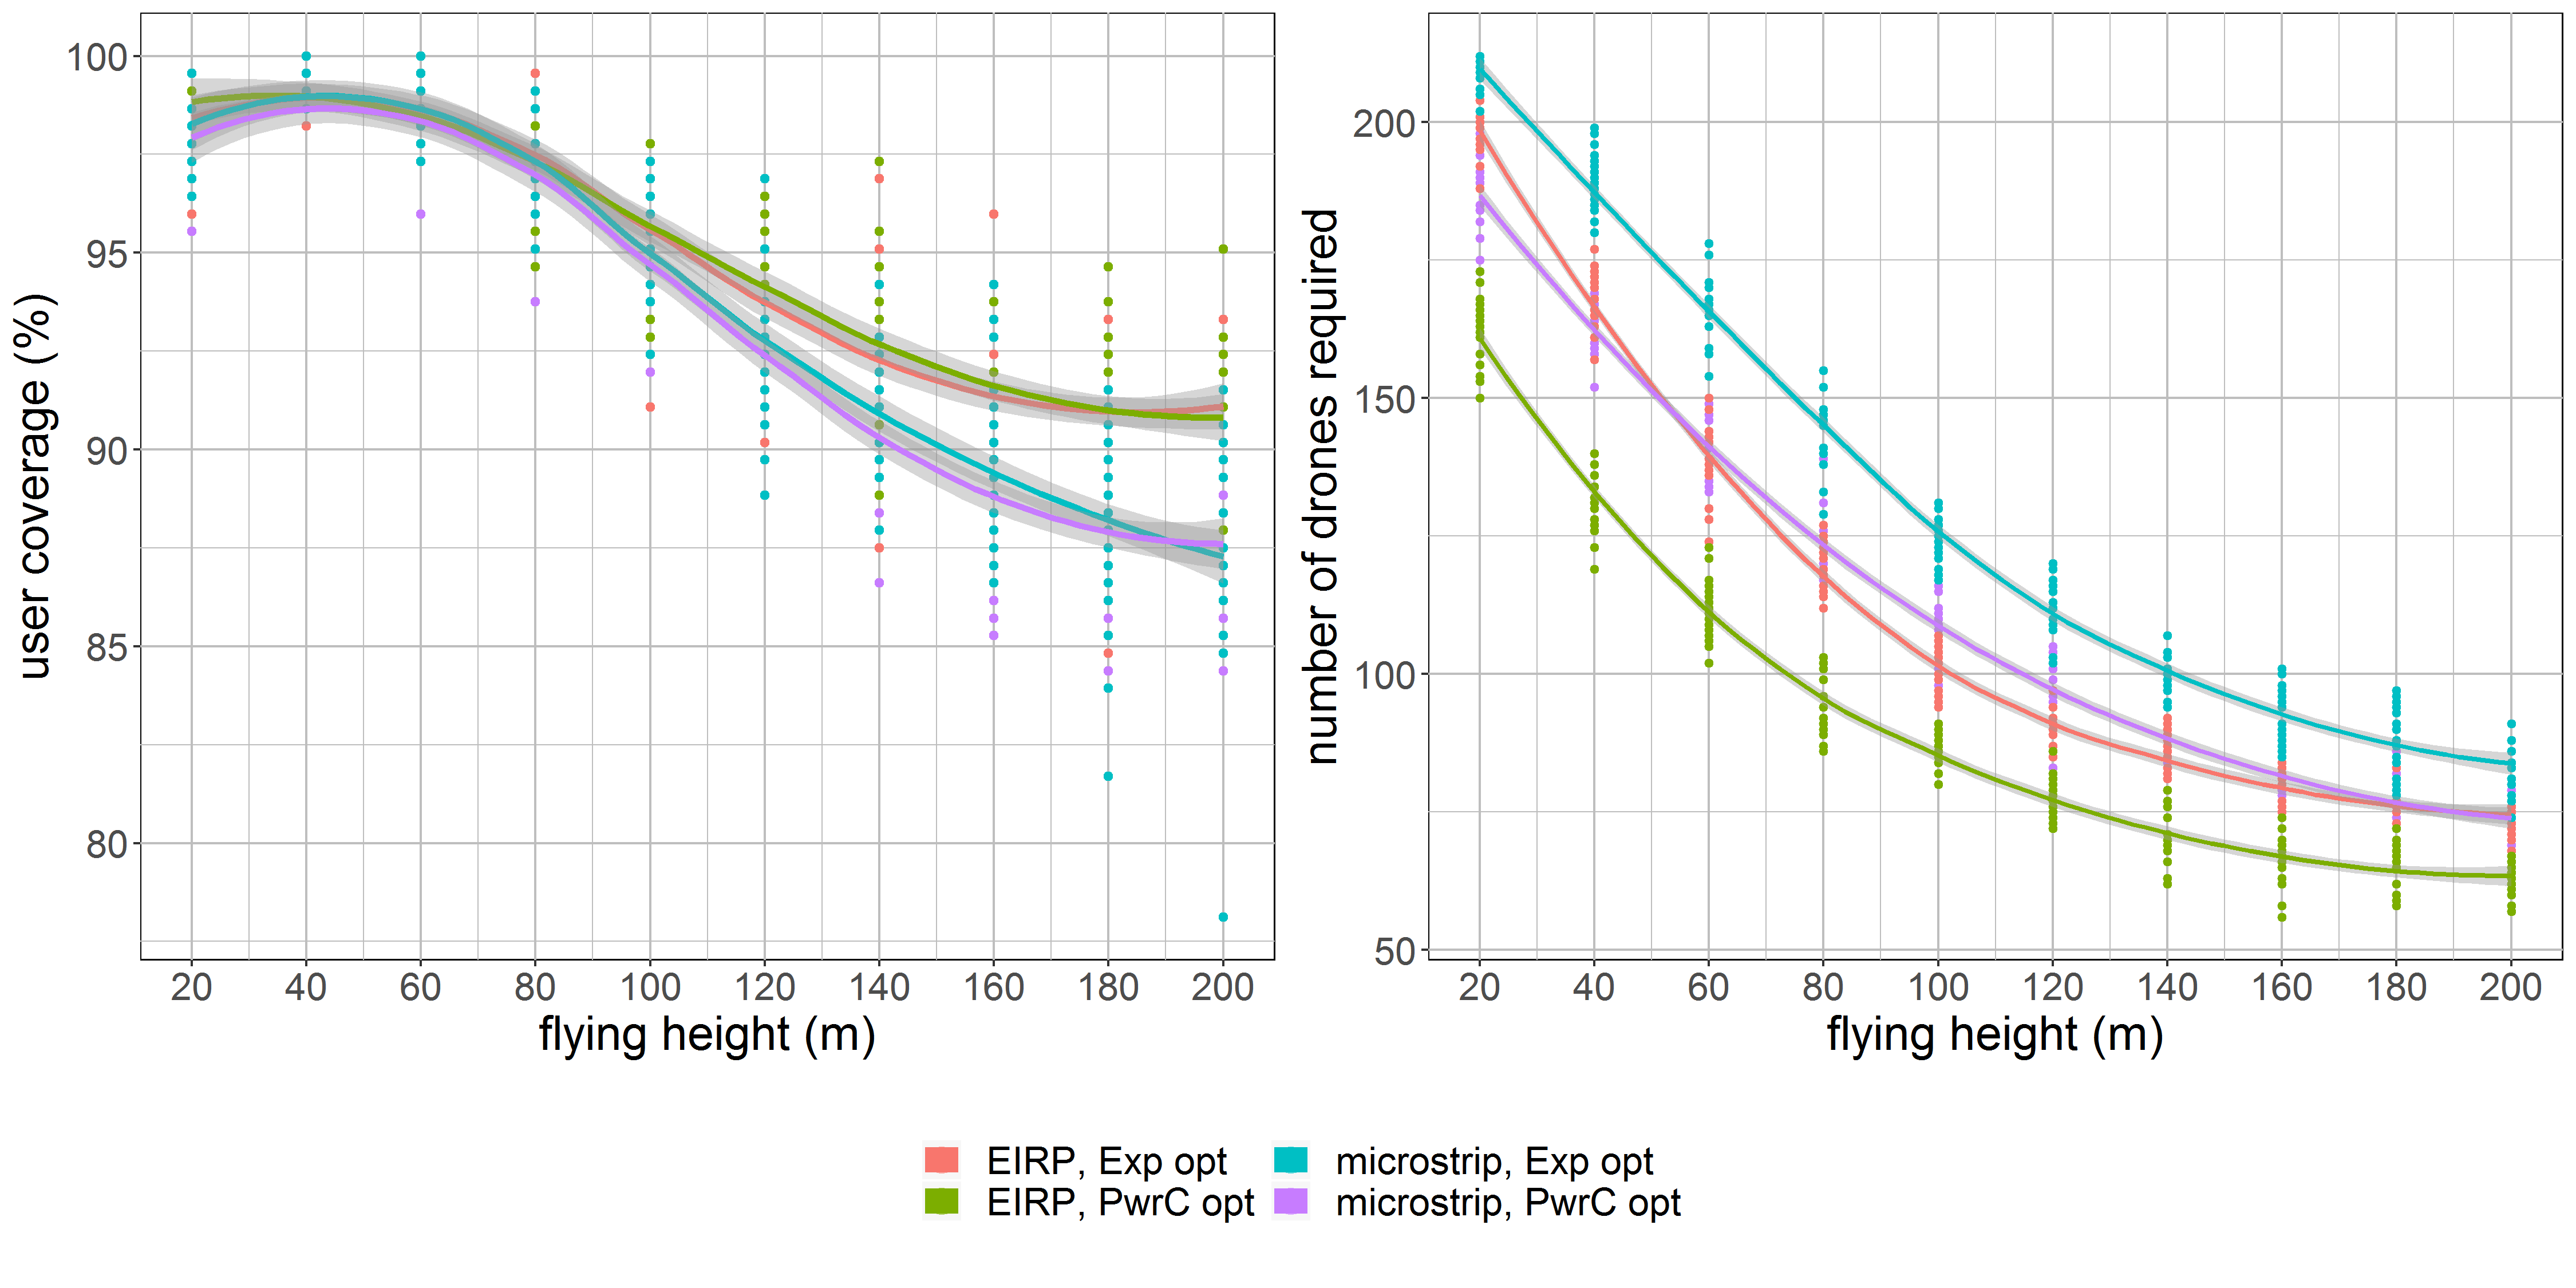
\includegraphics[width=\textwidth]{../results/s3/fhvsnumdronesAndCov.png}
  \caption{This graph shows how much \acs{UAV}s are required at different flying heights while trying to achieve a 100\% coverage.}
  \label{fig:s3a_numDronesAndCov}
\end{figure}

Scenario I already proved that for low altitude \gls{UAV}s, the main source of electromagnetic radiation are \gls{UABS}s. 
This changed around 80 metres where \gls{UL} electromagnetic radiation of the \gls{UE}
exceeds \gls{DL} radiation in order to still be able to reach the high flying \gls{UABS}s. 
When looking at the individual sources of electromagnetic exposure presented in figure \ref{fig:s3a_fourSourcesMatrix}, 
we notice the same behaviour where the 
 \gls{SAR} from the own device indeed increases between 89 and 141 $nW/kg$ by raising the flying altitude from 
 20 to 200 metres.
 % micro pc = 107 nw/kg (9 times more); micro exp = 124 nw/kg(15 times more); eirp exp = 141nw/kg (11 times more); eirp pc=89 nw/kg (2.5 times more)
  However, a more logarithmic increase is shown
  despite the fact that figure \ref{fig:s1_fhsar} showed an exponential increase.
This was however deducted with only one user present in the network as opposed to this scenario 
where 224 users are present. 
The electromagnetic radiation from the covered users will still behave like it did in Scenario I.
Moreover, the \gls{SAR} shown in figure  \ref{fig:s1_fhsar} is averaged  over covered and uncovered users.
In conclusion, the average  \gls{UL} \gls{SAR} in  figure \ref{fig:s1_fhsar} will not increase as fast as it did
in Scenario I (fig. \ref{fig:s1_fhsar}).

We can see from figure \ref{fig:s3a_fourSourcesMatrix} that once the flying altitude surpasses the \gls{NLOS} of the buildings, 
around 70 to 80 metres, the SAR from the serving \gls{UABS} remains 
more or less constant for all configurations.
The $SAR^{myUABS}$ varies for flying heights between 80 and 200 metres
around $160\ nW/kg$ for microstrip \gls{PwrC Opt} networks and around $98\ nW/kg$ for microstrip \gls{Exp Opt} and \gls{EIRP} \gls{PwrC Opt} networks.
An \gls{EIRP} \gls{Exp Opt} network is situated around $47\ nW/kg$.

When looking at the exposure from `other \gls{UABS}s', an increase in electromagnetic radiation at higher 
flying altitudes is noticed.
The lower path loss from less obstructing buildings will be the reason.
The figures from \ref{fig:s3a_fourSourcesMatrix} clearly show that this increase 
in electromagnetic radiation will be less for a microstrip patch antenna. The reason behind this is that energy 
will be more focused towards the ground and there is less sideways radiation because of attenuation.
The results show that by raising the flying altitude from 20 to 200 metres,
the $SAR^{otherUABS}$ will increase between 115 and 140 $nW/kg$ for \gls{EIRP} antennae and between 54 and 74 $nW/kg$ for microstrip patch antennae.
\clearpage
\begin{figure}[]
\centering
  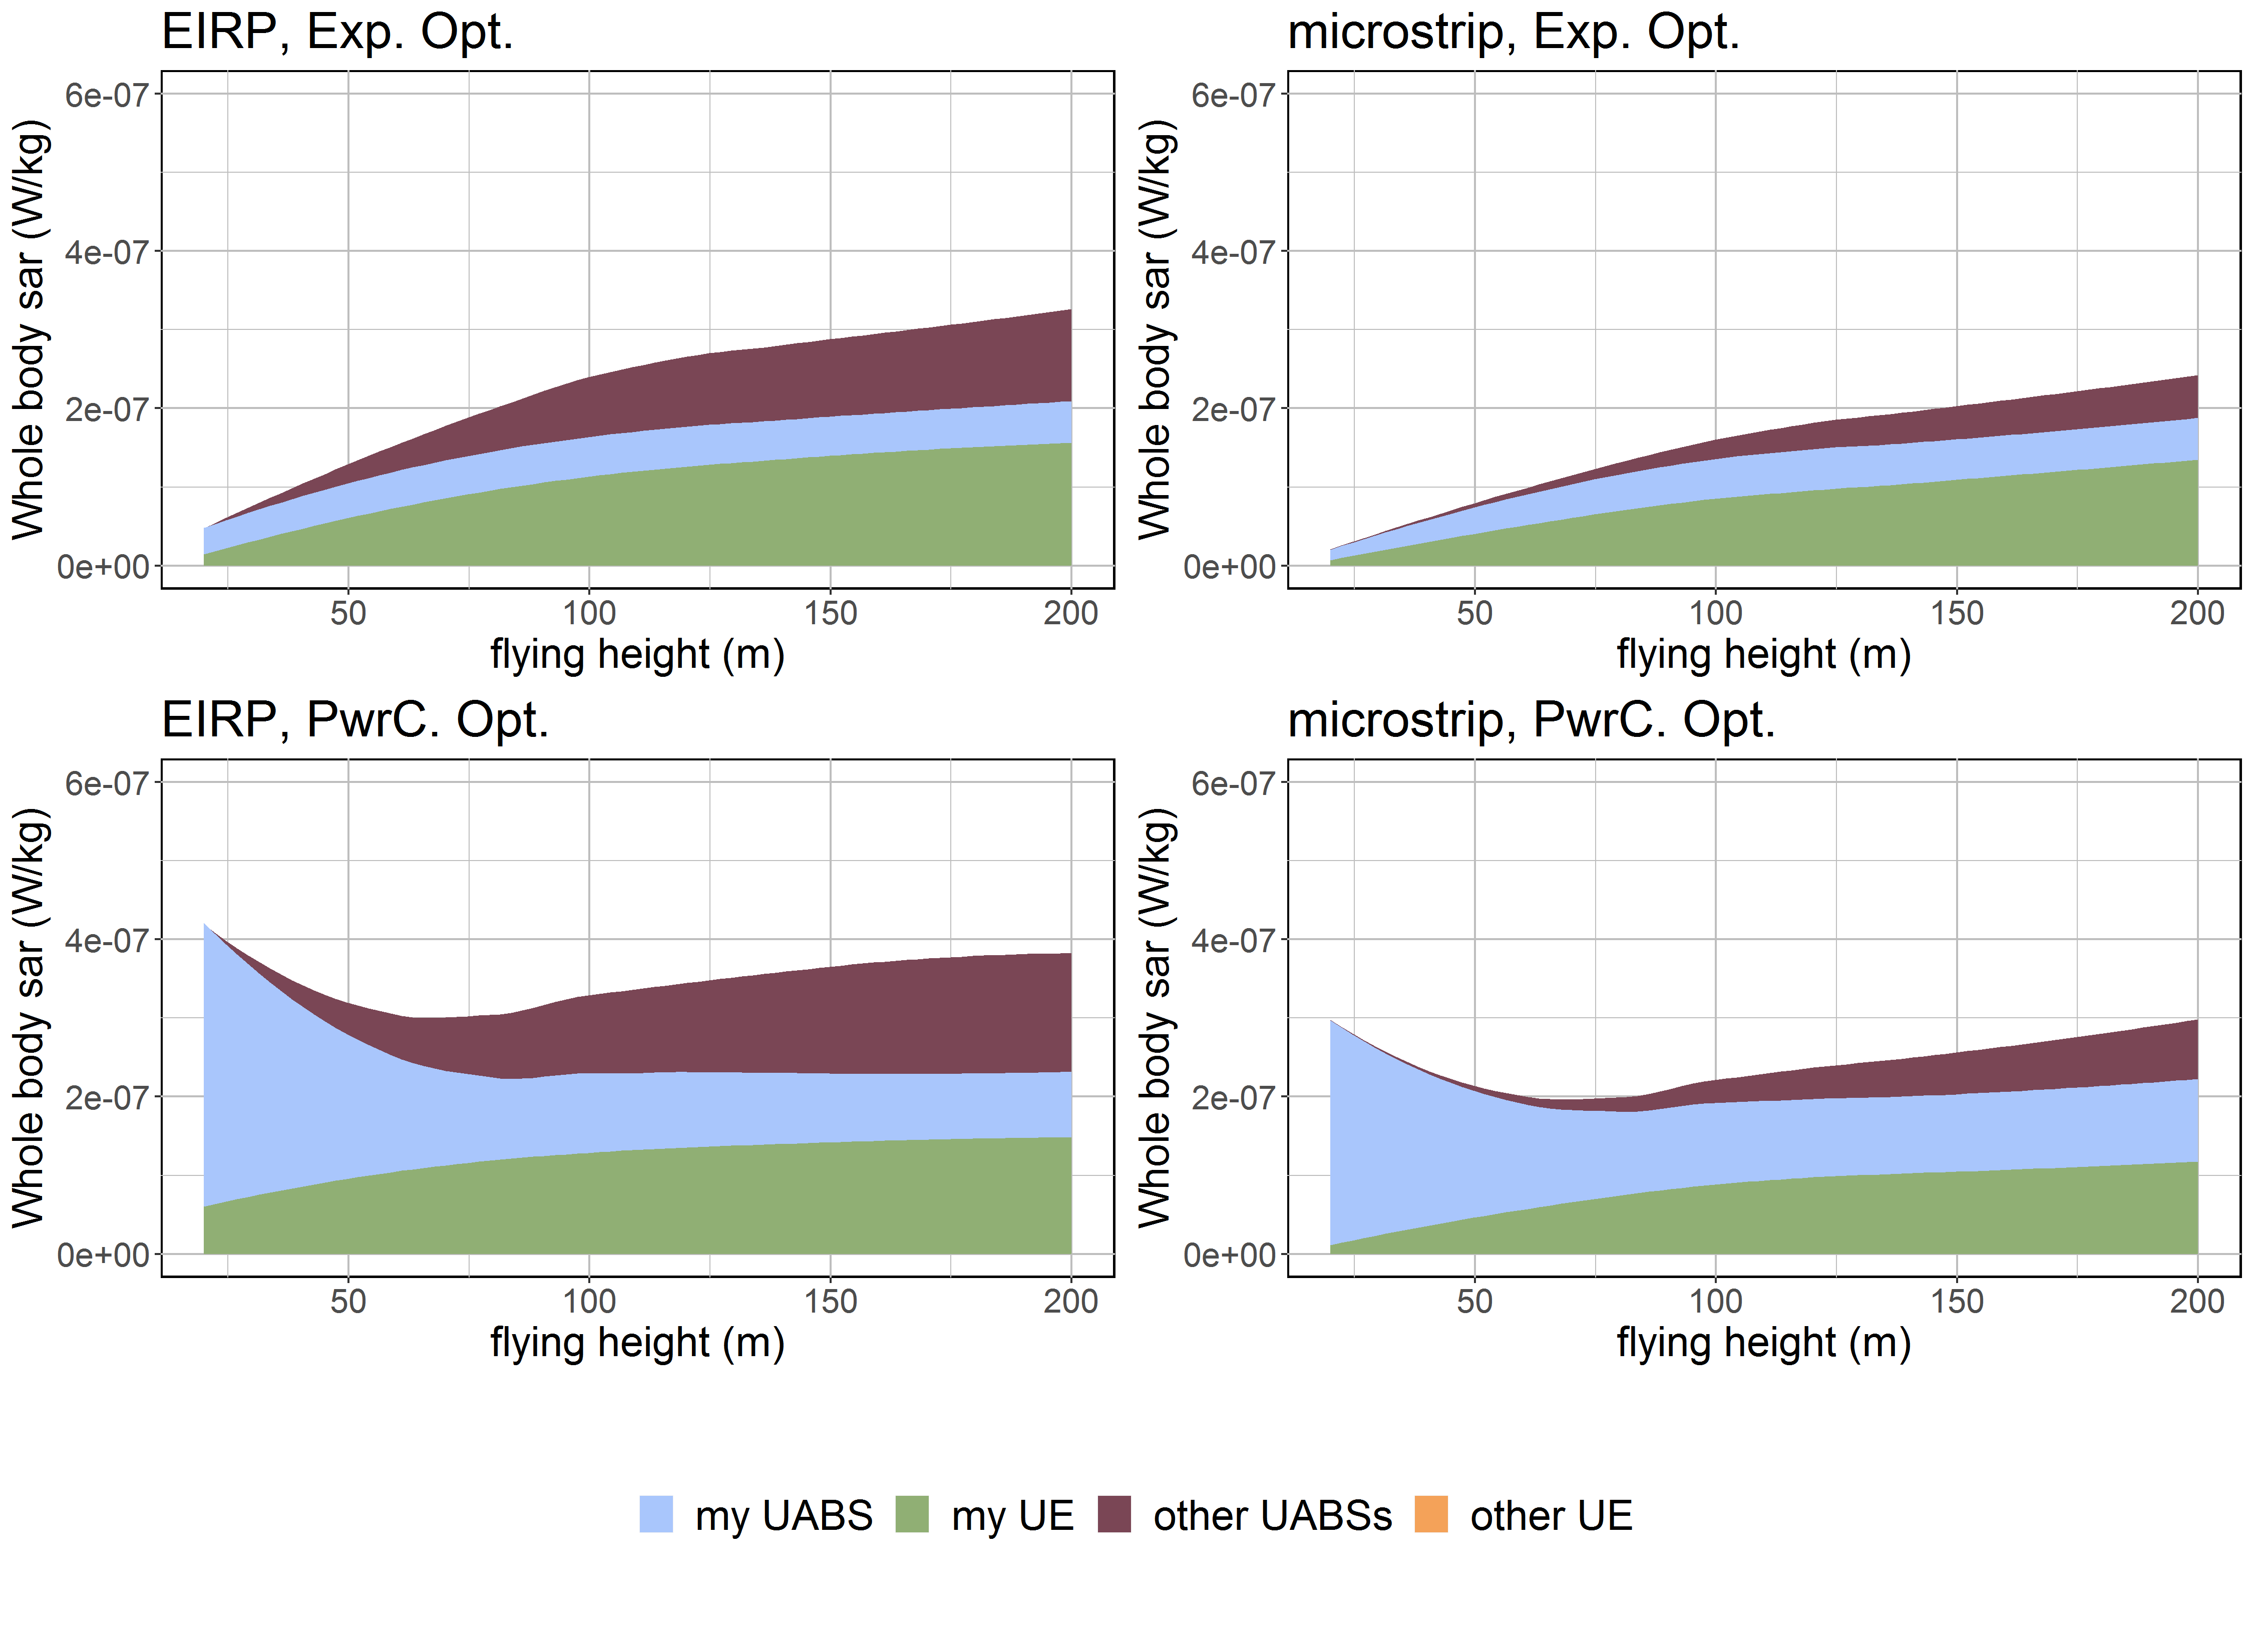
\includegraphics[width=\textwidth]{../results/s3/fhFourSources.png}
  \caption{
  Each figure corresponds with a certain configuration and shows how the \acs{SAR} from different sources are influenced by an increasing flying height.}  
  \label{fig:s3a_fourSourcesMatrix}
\end{figure}

%%%%%%%%%%%%%%%%%%%%%%%%%%%%%%%%%%%%%%%%%%%%%%%%%%%%%%%%%%%%%%%%%%%%%%%%%%%%%
\FloatBarrier
\subsection{Influence of the Number of Users}
\label{S3B}
The second evaluated parameter of Scenario III is a variable number of users while the flying height is fixed to 100 metres.  
Figure \ref{fig:s3b_numdronesAndCov}.a shows how the tool tries to reach a 100\% coverage. The percentage
of covered users is slightly less for smaller networks. For only 50 users, an average 
coverage of around 93\% is achieved while a network with 600 users has a coverage of around 97\%.
Figure \ref{fig:s3b_numdronesAndCov}.b shows how the tool requires more \gls{UAV}s for these large 
populations. 
The difference in optimization strategy is very little for a small amount of people but increases very quickly. 
When the population increases from 50 to 600 users,
 200 more \gls{UABS}s are required by a microstrip \gls{Exp Opt} network 
 around 130 more \gls{UABS}s for an \gls{EIRP} \gls{Exp Opt} network or a microstrip \gls{PwrC Opt} network
 and 110 more \gls{UABS}s for an \gls{EIRP} \gls{PwrC Opt} network.
This is an expected behaviour  when looking at Scenario II where, with only one \gls{UABS} available, 
the percentage of covered users decreases for these larger populations.
\clearpage
\begin{figure}[h]
  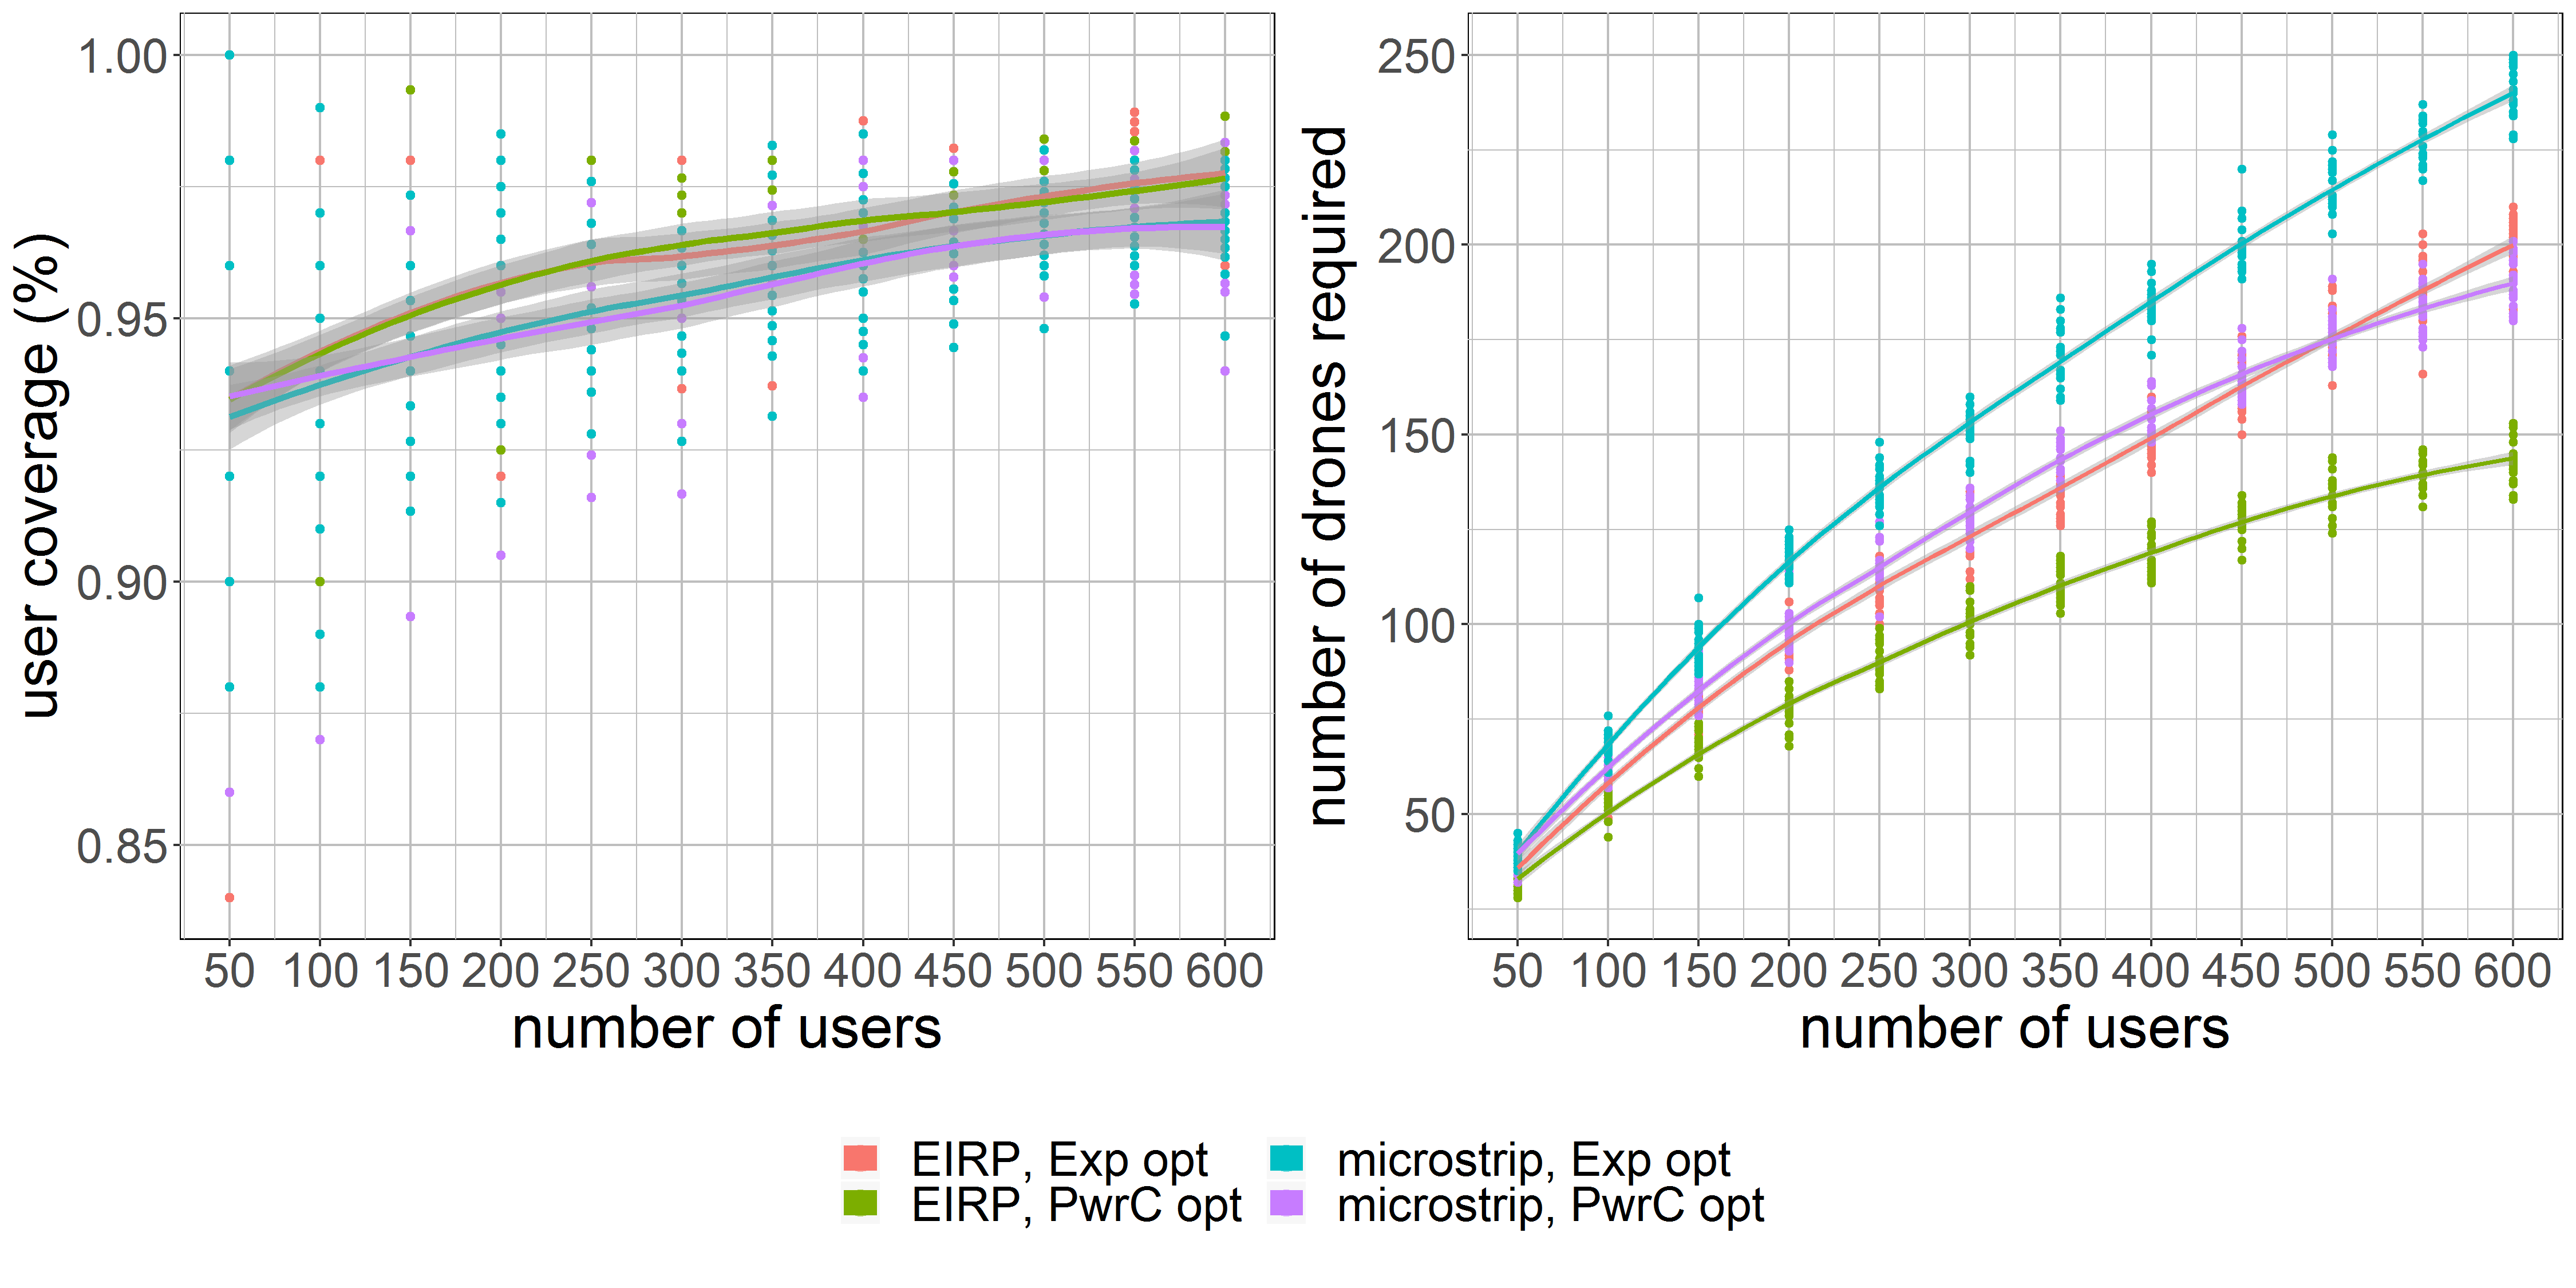
\includegraphics[width=\textwidth]{../results/s3/uvsnumdronesAndCov.png}
  \caption{This graph shows how much \acs{UAV}s are required for different flying heights while trying to achieve a 100\% coverage.}
  \label{fig:s3b_numdronesAndCov}
\end{figure}

Figure \ref{fig:s3b_dlAndPC} shows that the electromagnetic radiation and power consumption increase for larger 
populations which is normal since more drones will be available.
When the population increases from 50 to 600 users, the electromagnetic radiation increases 
between 80 and 130 $mV/m$ depending on the configuration. The power consumption with 50 users is for all configurations around 
20 $W$. Once the population is increased to 600 users, a microstrip \gls{Exp Opt} network will require 130 $W$, 
 a microstrip \gls{PwrC Opt} network requires 117 $W$,
\gls{EIRP} \gls{Exp Opt} networks require 107 $W$ and \gls{EIRP} \gls{PwrC Opt} network requires 92 $W$.

The correct behaviour of the decision algorithm became already clear in the previous subsection \ref{S3A} but is also
confirmed here. 
When comparing both optimization strategies, a power consumption optimized network requires around 5 $W$ less but exposes its users between 27 $mV/m$ and 30 $mV/m$ more than
exposure optimized networks. 
Further, it is also noticed that \gls{isotropicradiator}s cause more electromagnetic radiation for less energy
compared to microstrip patch antennae. 
When comparing the two types of antennae for a default number of 224 users, 
an \gls{isotropicradiator} will expose the average user 
between 25 $mV/m$ and 27 $mV/m$ more while requiring around 12 $W$ less than when the network would be using a microstrip patch antennae.


\begin{figure}[h!]
  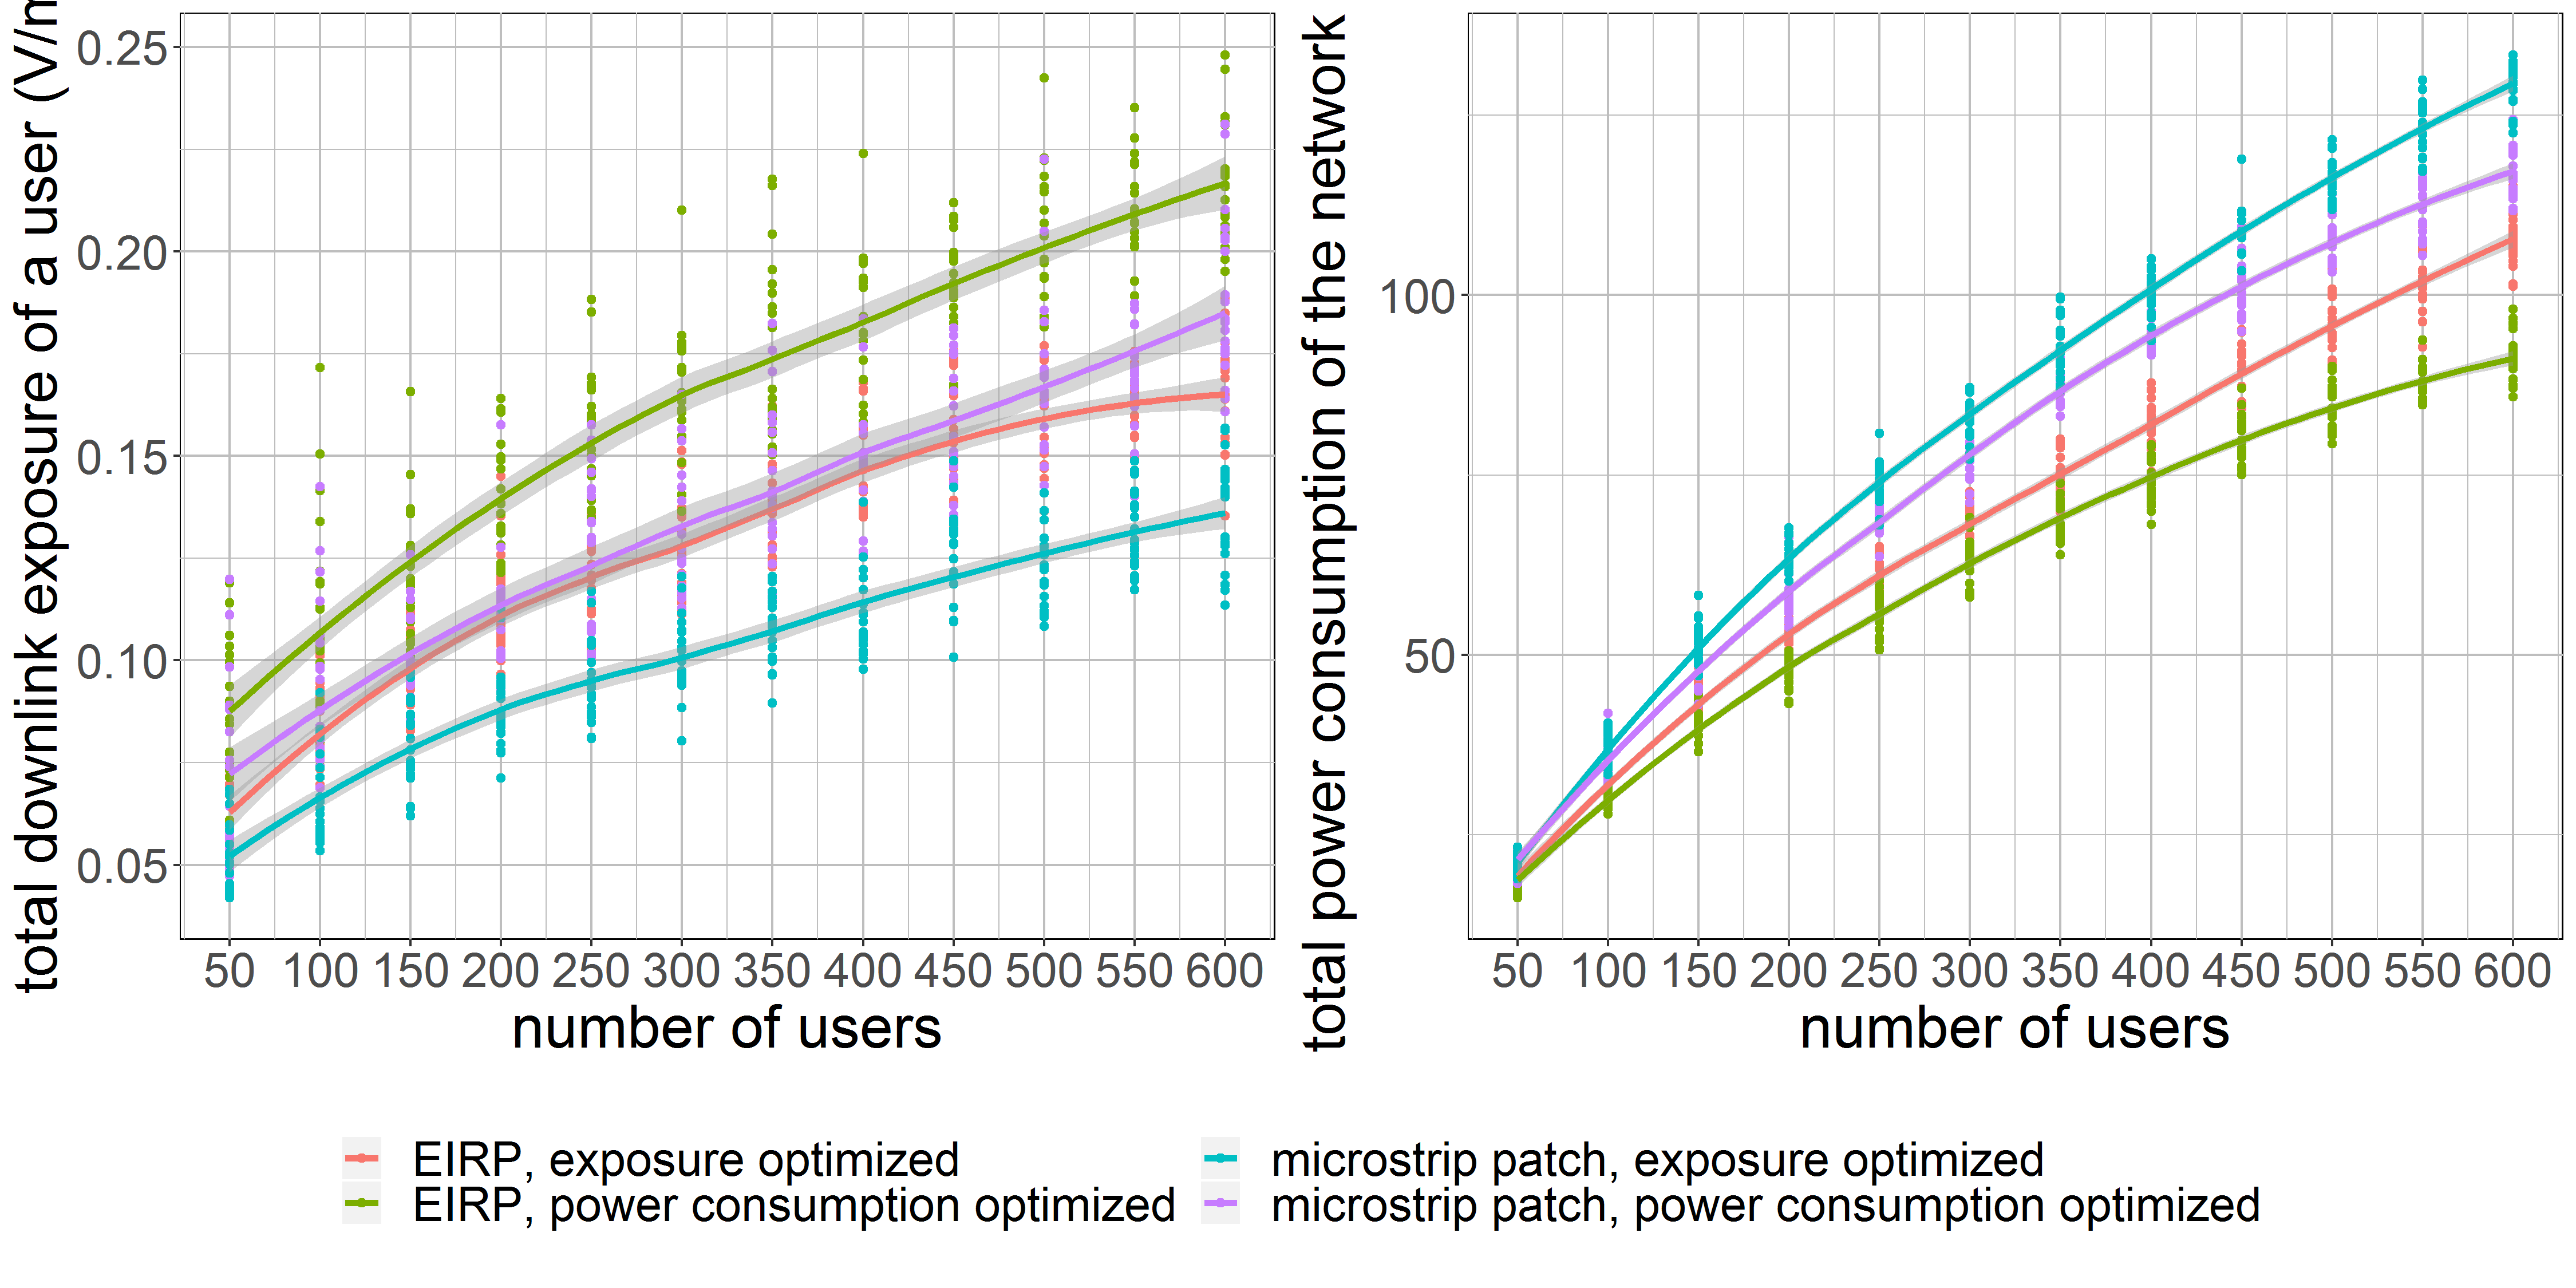
\includegraphics[width=\textwidth]{../results/s3/uvsdlAndPc.png}
  \caption{The influence of the population size on the downlink electromagnetic radiation (a) and power consumption (b).}
  \label{fig:s3b_dlAndPC}
%\bigbreak
 % 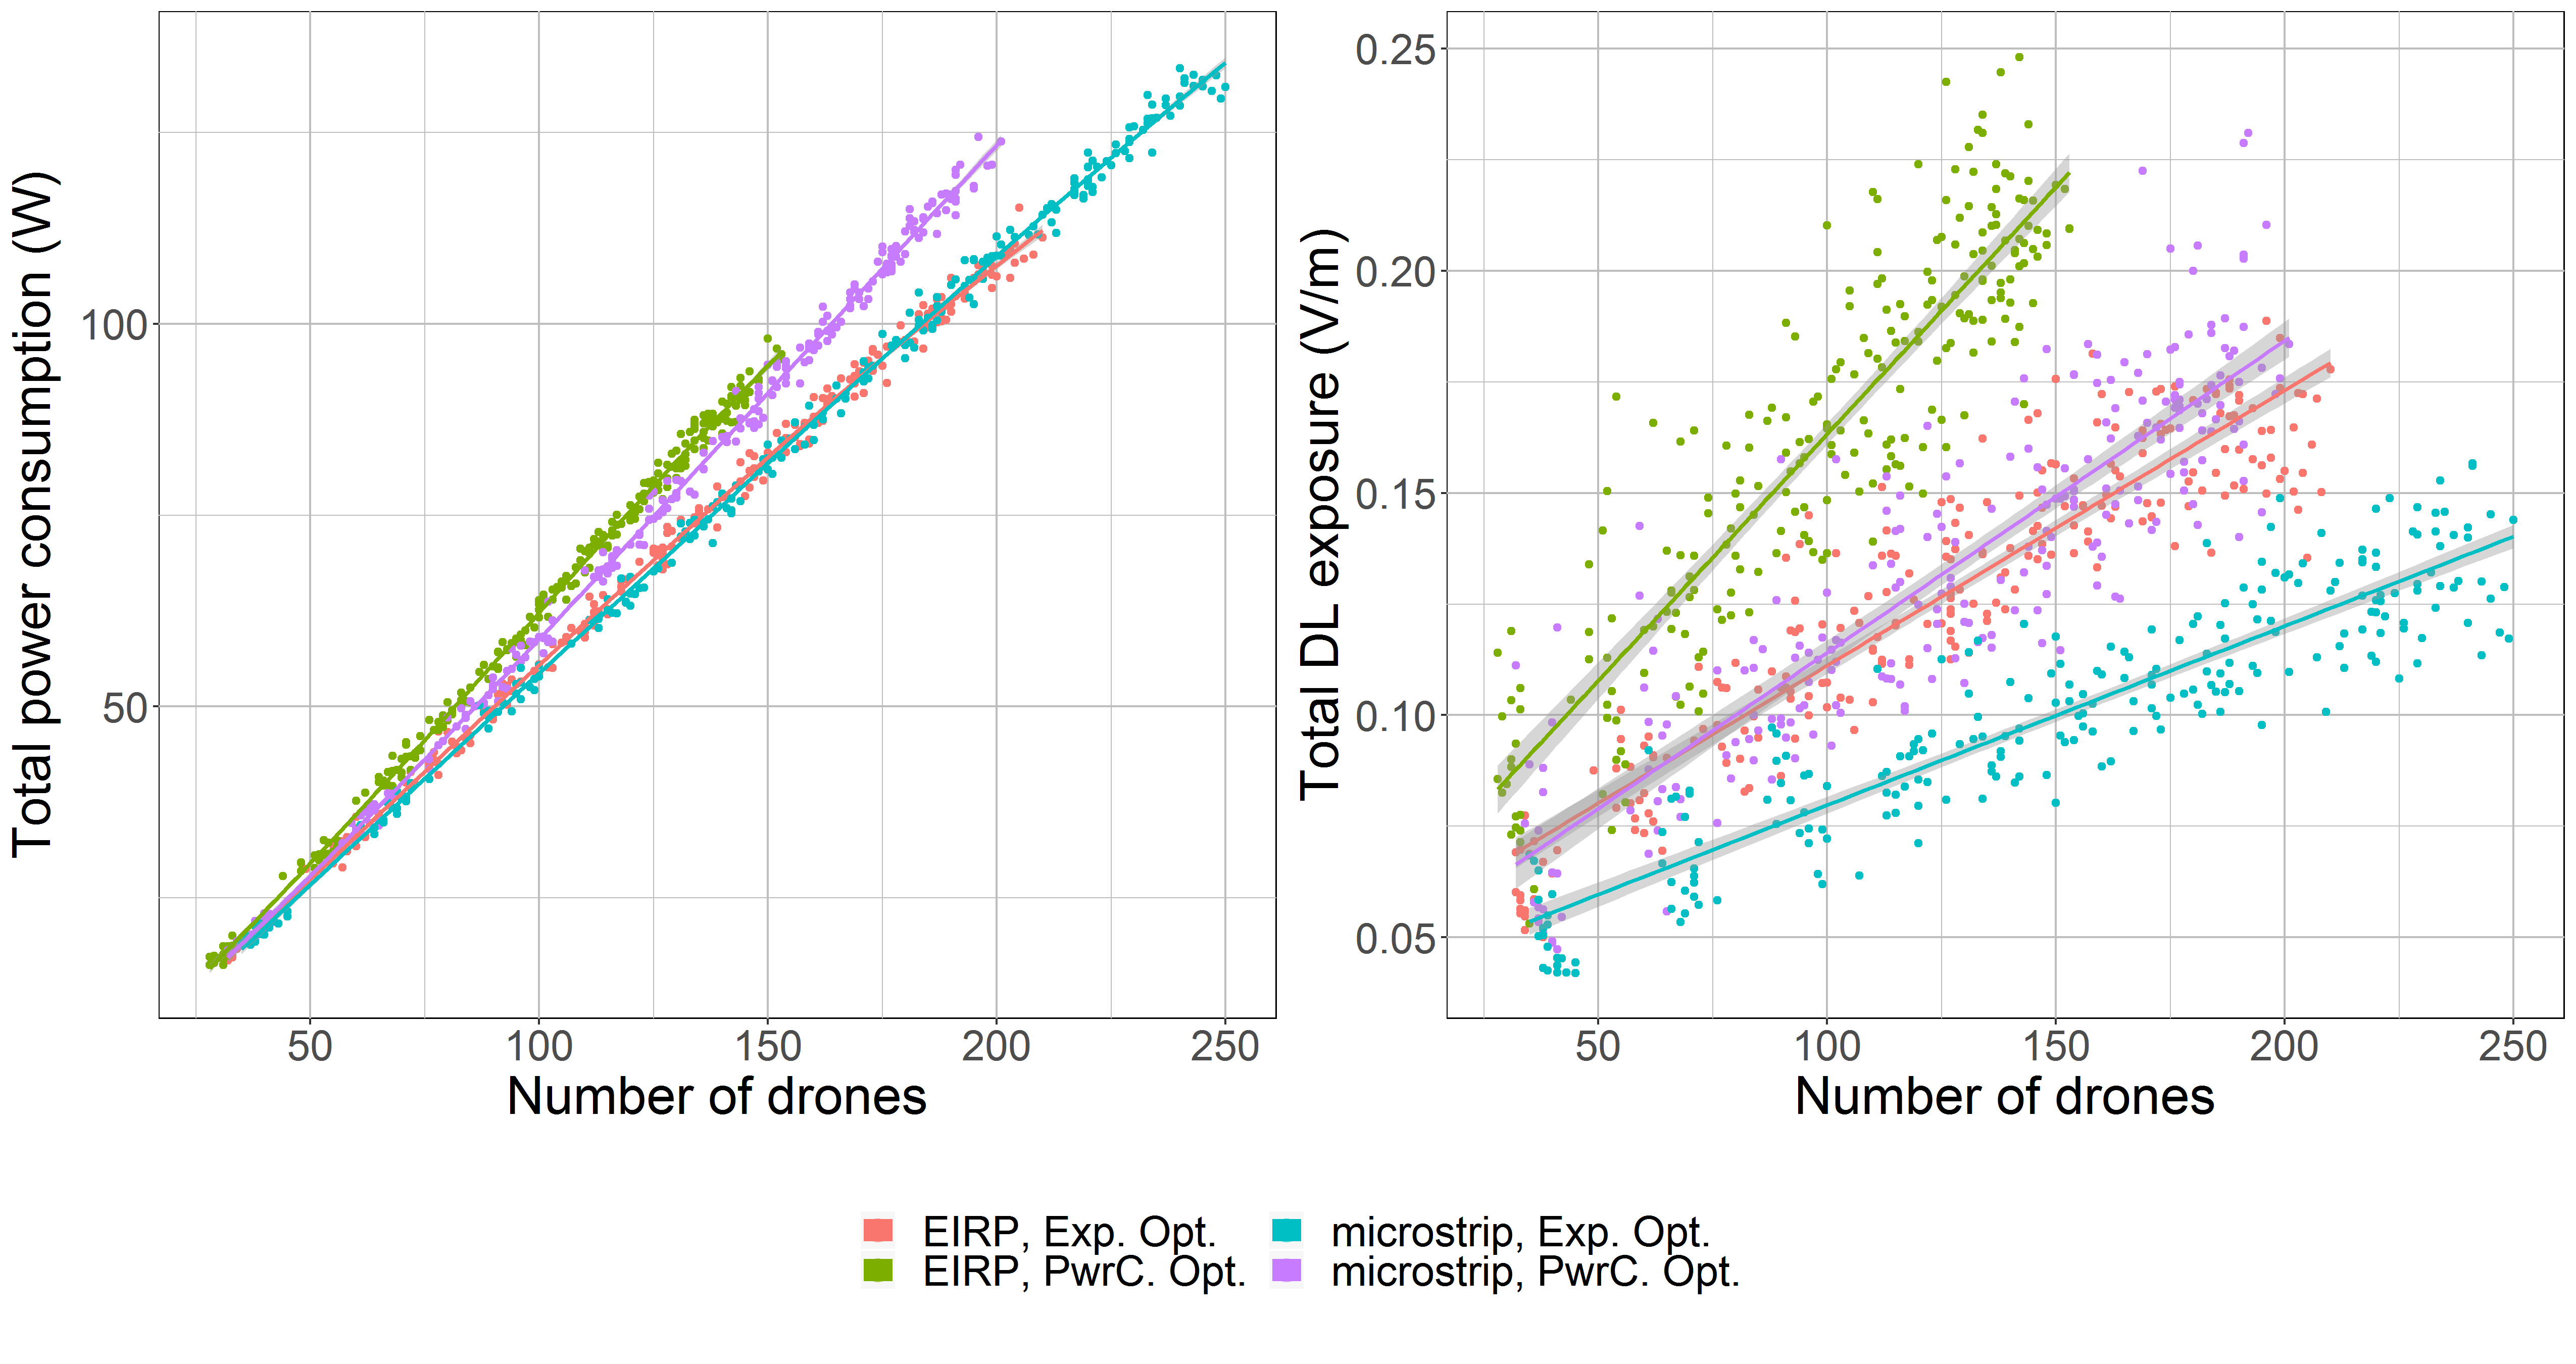
\includegraphics[width=\textwidth]{../results/s3/u_numdronesvsdlAndPc.png}
  %\caption{The influence of the number of UABSs on the downlink electromagnetic radiation (a) and power consumption (b).}
  %\label{fig:s3b_dlAndPC2}
\end{figure}
This means that Scenario III confirms that a power consumption optimized network indeed results in less \gls{UAV}s and a lower 
 power consumption for the entire network. 
At the same time, Scenario II showed that the active \gls{UABS}s have a higher individual power consumption.
We can therefore state that a power consumption optimized network will reduce its total power consumption by
using a few high powered \gls{UAV}s.
Likewise for an exposure optimized network, we can conclude that the network has indeed a lower electromagnetic exposure but the power consumption 
of the entire network is much higher. In Scenario II became already clear that the active \gls{UABS}s have a low power consumption in order to 
guarantee a low electromagnetic exposure towards the users.
We can conclude that an exposure optimized network will reduce the exposure of an individual 
by deploying several low powered \gls{UABS}s.

Figure \ref{fig:s3b_fourSourcesMatrix} shows how the  $SAR^{ownUE}$  
remains almost constant which is normal since the flying height remains the same and will 
vary between  0.7 $\mu W/kg$ and 1.2 $\mu W/kg$.
The $SAR^{myUABS}$ barely increases in an exposure optimized network and is situated around 0.5 $\mu W/kg$ for both antennae.
The power consumption optimized network also starts around 0.5 $\mu W/kg$ but increases when more users become online. 
A normal behaviour when considering that these \gls{UABS}s try to cover much more users. Therefore, the $SAR^{myUABS}$ 
with 600 users increases up to 2 $\mu W/kg$ depends on the configuration.
The \gls{SAR} value that increases the most is $SAR^{otherUABS}$ which 
starts really low with less than 0.1 $\mu W/kg$ for 50 users for all configurations. 
The \gls{SAR} increases however very fast. The biggest increase is noticed in an \gls{EIRP} \gls{PwrC Opt} network 
where 3 $\mu W/kg$ is measured for 600 users. The $SAR^{otherUE}$ increases the least for microstrip \gls{Exp Opt} with 
only 1 $\mu W/kg$ for 600 users.
\begin{figure}[h!]
\centering
  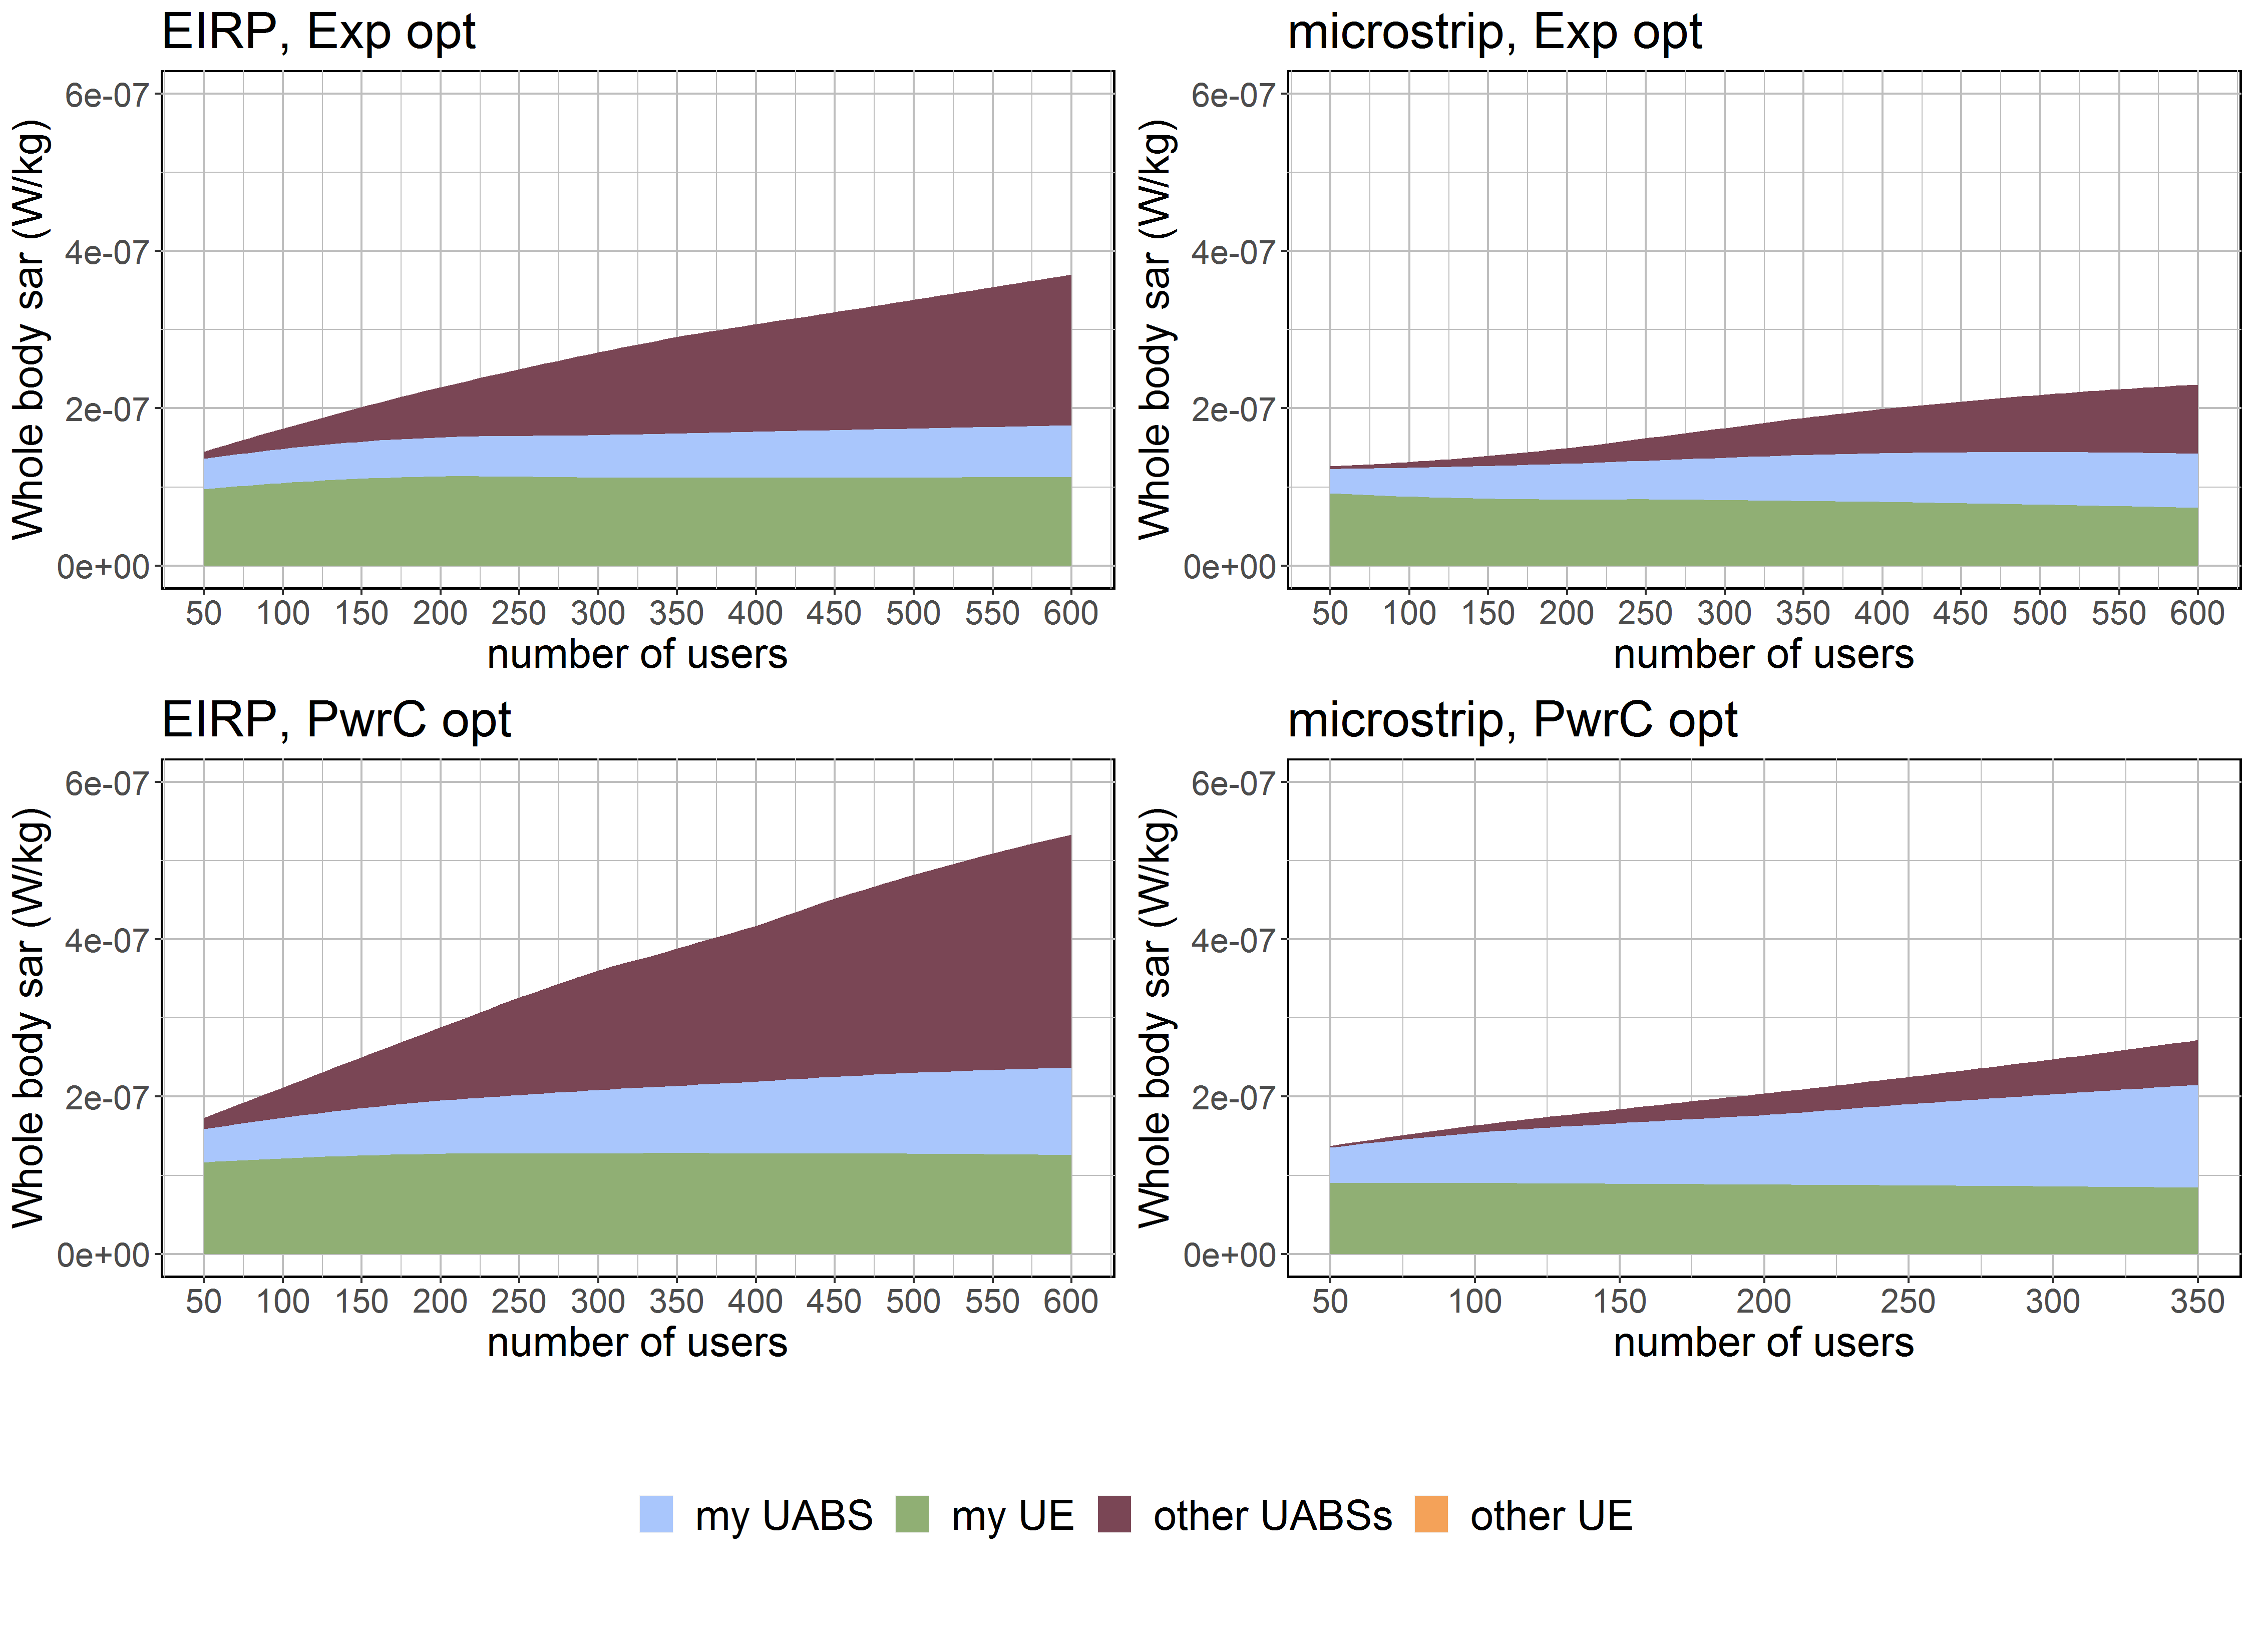
\includegraphics[width=0.9\textwidth]{../results/s3/uFourSources.png}
  \caption{Each figure shows the \acs{SAR} from different sources for an increasing population size. 
}
  \label{fig:s3b_fourSourcesMatrix}
\end{figure}

\section{Summary}
This chapter discusses the achieved results when applying the tool to the different scenarios.
Scenario I concludes that the required transmission power increases logarithmically with the flying height.
The results show how the user's device is the main source of electromagnetic radiation 
for all flying heights above 80 metres and grows exponentially along with the flying height. 
On the other hand, the electromagnetic 
radiation from the \gls{UABS} remains constant around 10 $nW/kg$.
Scenario II shows that electromagnetic exposure  drops when the population size increases or when the flying height decreases
and a lower user exposure corresponds with lower coverage. Users that are covered are, just like in Scenario I, 
mainly exposed to their own device, followed by the \gls{UABS} in second place. The results also show that 
the power consumption slightly increases when the \gls{UABS} covers more users.
The last scenario shows that less \gls{UABS}s are required for higher flying altitudes and therefore 
result in a decreased power consumption.  Exposure from the serving \gls{UABS} remains almost constant above 80 metres while 
exposure from other \gls{UABS}s and \gls{UE} increases. Scenario III also shows that more \gls{UABS}s are 
required for larger populations and therefore increase power consumption and electromagnetic exposure.
Finally, the results also confirm that the optimization algorithm works as intended 
and is able to optimize towards either electromagnetic exposure or overall power consumption.

\begin{table}[]
\begin{tabular}{|l|l|l|l|l|}
\hline
\textbf{Scenario}                      & \textbf{Configuration}                   & \textbf{Network power consumption (W)} & \textbf{DL Exposure (V/m)} & \textbf{WB SAR (W/kg)} \\ \hline
\multirow{2}{*}{\textbf{Scenario I}}   & \textbf{\acs{Exp Opt}}                   &                                    &                   &                \\ \cline{2-5} 
                                       & \textbf{\acs{PwrC Opt}}                  &                                    &                   &                 \\ \hline
\multirow{4}{*}{\textbf{Scenario II}}  & \textbf{EIRP \acs{Exp Opt}}              &                                    &                   &                 \\ \cline{2-5} 
                                       & \textbf{EIRP \acs{PwrC Opt}}             &                                    &                   &                 \\ \cline{2-5} 
                                       & \textbf{microstrip \acs{Exp Opt}}        &                                    &                   &                 \\ \cline{2-5} 
                                       & \textbf{microstrip \acs{PwrC Opt}}       &                                    &                   &                 \\ \hline
\multirow{4}{*}{\textbf{Scenario III}} & \textbf{EIRP \acs{Exp Opt}}              &                                    &                   &                 \\ \cline{2-5} 
                                       & \textbf{EIRP \acs{PwrC Opt}}             &                                    &                   &                 \\ \cline{2-5} 
                                       & \textbf{microstrip \acs{Exp Opt}}        &                                    &                   &                 \\ \cline{2-5} 
                                       & \textbf{microstrip \acs{PwrC Opt}}       &                                    &                   &                 \\ \hline
\end{tabular}
\end{table}